% \iffalse meta-comment
%
% Copyright (C) 2021- by LIWenhui <lwh@hrbeu.edu.cn>
%
% This file may be distributed and/or modified under the
% conditions of the LaTeX Project Public License, either version 1.3a
% of this license or (at your option) any later version.
% The latest version of this license is in:
%
% http://www.latex-project.org/lppl.txt
%
%
% \fi
%
% \iffalse
%<*driver>
\ProvidesFile{heuthesis.dtx}[2021/12/06 1.0.0 Harbin Engineering University Thesis Template]
\documentclass{ltxdoc}
\usepackage{dtx-style}

\EnableCrossrefs
\CodelineIndex
\RecordChanges

\begin{document}
  \DocInput{\jobname.dtx}
\end{document}
%</driver>
% \fi
%
% \CheckSum{0}
%
% \CharacterTable
%  {Upper-case    \A\B\C\D\E\F\G\H\I\J\K\L\M\N\O\P\Q\R\S\T\U\V\W\X\Y\Z
%   Lower-case    \a\b\c\d\e\f\g\h\i\j\k\l\m\n\o\p\q\r\s\t\u\v\w\x\y\z
%   Digits        \0\1\2\3\4\5\6\7\8\9
%   Exclamation   \!     Double quote  \"     Hash (number) \#
%   Dollar        \$     Percent       \%     Ampersand     \&
%   Acute accent  \'     Left paren    \(     Right paren   \)
%   Asterisk      \*     Plus          \+     Comma         \,
%   Minus         \-     Point         \.     Solidus       \/
%   Colon         \:     Semicolon     \;     Less than     \<
%   Equals        \=     Greater than  \>     Question mark \?
%   Commercial at \@     Left bracket  \[     Backslash     \\
%   Right bracket \]     Circumflex    \^     Underscore    \_
%   Grave accent  \`     Left brace    \{     Vertical bar  \|
%   Right brace   \}     Tilde         \~}
%
% \DoNotIndex{\newenvironment,\@bsphack,\@empty,\@esphack,\sfcode}
% \DoNotIndex{\addtocounter,\label,\let,\linewidth,\newcounter}
% \DoNotIndex{\noindent,\normalfont,\par,\parskip,\phantomsection}
% \DoNotIndex{\providecommand,\ProvidesPackage,\refstepcounter}
% \DoNotIndex{\RequirePackage,\setcounter,\setlength,\string,\strut}
% \DoNotIndex{\textbackslash,\texttt,\ttfamily,\usepackage}
% \DoNotIndex{\begin,\end,\begingroup,\endgroup,\par,\\}
% \DoNotIndex{\if,\ifx,\ifdim,\ifnum,\ifcase,\else,\or,\fi}
% \DoNotIndex{\let,\def,\xdef,\edef,\newcommand,\renewcommand}
% \DoNotIndex{\expandafter,\csname,\endcsname,\relax,\protect}
% \DoNotIndex{\Huge,\huge,\LARGE,\Large,\large,\normalsize}
% \DoNotIndex{\small,\footnotesize,\scriptsize,\tiny}
% \DoNotIndex{\centering,\raggedright,\ref}
% \DoNotIndex{\c@secnumdepth,\@startsection,\@setfontsize}
% \DoNotIndex{\ ,\@plus,\@minus,\p@,\z@,\@m,\@M,\@ne,\m@ne}
% \DoNotIndex{\@@par,\DeclareOperation,\RequirePackage,\LoadClass}
% \DoNotIndex{\AtBeginDocument,\AtEndDocument}
%
% \GetFileInfo{\jobname.dtx}
%
%
% \def\indexname{索引}
% \def\glossaryname{修改记录}
% \IndexPrologue{\section{\indexname}}
% \GlossaryPrologue{\section{\glossaryname}}
%
% \title{\bfseries\color{violet}\heuthesis:哈尔滨工程大学学位论文模板}
% \author{{\songti [\ 李文辉}\ ]\texttt{lwh@hrbeu.edu.cn}}
% \date{v\fileversion\ (\filedate)}
% \maketitle\thispagestyle{empty}
% \begin{abstract}\noindent
% 该宏包为哈尔滨工程大学本、硕、博中英文毕业论文、开题和中期报告以及博后出站报告模板。
% \end{abstract}
%
% \vskip2cm
% \def\abstractname{免责声明}
% \begin{abstract}
% \noindent
% \begin{enumerate}
% \item 本模板的发布遵守 \LaTeX\ Project Public License,使用前请认真阅读协议内容。
% \item 本模板为作者根据 \heu 教务处颁发的 \UGR ,\heu 研究生院颁发的 \PGR 
% 编写而成,为 \heu 学学生撰写毕业论文使用。
% \item \heu 教务处和研究生院只提供毕业论文写作指南,不提供官方模板,
% 也未授权第三方模板为官方模板,所以此模板仅为写作指南的参考实现,不保证格
% 式审查老师不提意见。任何由于使用本模板而引起的论文格式审查问题均与本模板作者无
% 关。
% \item 任何个人或组织以本模板为基础进行修改、扩展而生成的新的专用模板,请严格遵
%   守 \LaTeX\ Project Public License 协议。由于违犯协议而引起的任何纠纷争端均与
%   本模板作者无关。
% \end{enumerate}
% \end{abstract}
%
%
% \clearpage
% \pagestyle{fancy}
% \begin{multicols}{2}[
%   \setlength{\columnseprule}{.4pt}
%   \setlength{\columnsep}{18pt}]
%   \tableofcontents
% \end{multicols}
% \clearpage
%
% \section{模板介绍}
% \heuthesis\ (\textbf{H}arbin \textbf{E}ngineering \textbf{U}niversity \LaTeX\
% \textbf{Thesis} Template) 是为了帮助 \heu 毕业生撰写毕业论文而编写
% 的 \LaTeX\ 论文模板。
%
% 本模板是基于哈尔滨工业大学学位论文模板 \textsc{hi}\-\textsc{Thesis} 修改而来。
%
% 本文档将尽量完整的介绍模板的使用方法,如有不清楚之处可以参考示例文档或者根据
% 第~\ref{sec:howtoask} 节说明提问,有兴趣者都可以参与完善此手册,也非常欢迎对代
% 码的贡献。
%
% \note[注意:]{模板的作用在于减少论文写作过程中格式调整的时间。前提是遵守模板的
% 用法,否则即便用了 \heuthesis\ 也难以保证输出的论文符合学校规范。}
%
%
% \section{安装}
% \label{sec:installation}
% \heuthesis\ 一般不需要进行安装,直接将压缩包解压后就可以使用。
%
% \subsection{模板的组成}
% 下表列出了 \heuthesis\ 的主要文件及其功能介绍:
%
% \begin{longtable}{l|p{8cm}}
% \toprule
% {\heiti 文件(夹)} & {\heiti 功能描述}\\\midrule
% \endfirsthead
% \midrule
% {\heiti 文件(夹)} & {\heiti 功能描述}\\\midrule
% \endhead
% \endfoot
% \endlastfoot
% heuthesis.ins & \textsc{DocStrip} 驱动文件(开发用) \\
% heuthesis.dtx & \textsc{DocStrip} 源文件(开发用)\\\midrule
% heuthesisbook.cls & 模板类文件\\
% heuthesisbook.cfg & 模板配置文件\\
% heuthesis.bst & 参考文献样式文件\\\midrule
% heuthesis.ist & 索引样式文件\\\midrule
% reference.bib & 文档参考文献\\
% main.tex & 示例文档主文件\\
% front/ & 正文之前内容\\
% body/ & 正文内容\\
% back/ & 正文之后内容\\
% data/ & TiZk绘图数据文件\\
% figures/ & 插图图片路径\\
% heuthesis.sty & 为示例文档加载其它宏包\\\midrule
% Makefile & Makefile\\
% latexmkrc & latexmk 配置文件 \\
% README.md & Readme\\
% \textbf{heuthesis.pdf} & 用户手册(本文档)\\\bottomrule
% \end{longtable}
%
% 几点说明:
% \begin{itemize}
% \item \file{heuthesisbook.cls} 和 \file{heuthesisbook.cfg} 可由 \file{heuthesis.ins}
%   和 \file{heuthesis.dtx} 生成。
% \item 使用前阅读文档:\file{heuthesis.pdf}。
% \item 默认的生成的论文中含有丰富的格式示例,使用前请仔细阅读\file{main.pdf}。
% \end{itemize}
%
% \subsection{生成模板}
% \label{sec:generate-cls}
% 将模板解压缩到文件夹,
% 其中包括:模板源文件(\file{heuthesis.ins} 和 \file{heuthesis.dtx}),参考文献
% 样式 \file{heuthesis.bst} 和示例文档。在使用之前需要先生成模
% 板文件和配置文件(具体命令细节请参考 \file{README.md} 和 \file{Makefile}):
%
% 如果是直接使用编译后的模板文件,可以忽略下述操作。
%
% \begin{shell}
% $ cd heuthesis
% # 生成 heuthesisbook.cls 和 heuthesisbook.cfg
% $ xelatex heuthesis.ins
%
% # 下面的命令用来生成用户手册,可以不执行
% $ xelatex heuthesis.dtx
% $ makeindex -s gind.ist -o heuthesis.ind heuthesis.idx
% $ makeindex -s gglo.ist -o heuthesis.gls heuthesis.glo
% $ xelatex heuthesis.dtx
% $ xelatex heuthesis.dtx  % 生成说明文档 heuthesis.pdf
% \end{shell}
%
% \subsection{生成论文}
% \label{sec:generate-thesis}
% 本节介绍几种常见的生成论文的方法。用户可根据自己的情况选择。
%
% \subsubsection{\XeLaTeX}
% \label{sec:xelatex}
% 很多用户对 \LaTeX\ 命令执行的次数不太清楚。一个基本的原则是多次运行 \LaTeX\ 命
% 令直至不再出现警告。下面给出生成示例文档的详细过程(\texttt{\#} 开头的行为注
% 释),首先来看推荐的 \texttt{xelatex} 方式:
% \begin{shell}
% # 1. 发现里面的引用关系,文件后缀 .tex 可以省略
% $ xelatex main
%
% # 2. 编译参考文件源文件,生成 bbl 文件
% $ bibtex main
%
% # 3. 下面解决引用
% $ xelatex main
% $ xelatex main   # 如果不需要生成索引此时生成完整的 pdf 文件
% $ splitindex main -- -s heuthesis.ist  # 自动生成索引
% $ xelatex main.tex
% \end{shell}
%
% \subsubsection{latexmk}
% \label{sec:latexmk}
% \texttt{latexmk} 命令支持全自动生成 \LaTeX\ 编写的文档,并且支持使用不同的工具
% 链来进行生成,它会自动运行多次工具直到交叉引用都被解决。下面给出了一个用
% \texttt{latexmk} 调用 \texttt{xelatex} 生成最终文档的示例:
% \begin{shell}
% # 一句话就够了!
% $ latexmk -xelatex main
% \end{shell}
%
% \subsubsection{make}
% \label{sec:make}
%
% 上面的方法虽然不复杂,但是每次都输入还是非常罗嗦,所以 \heuthesis\ 提供了一
% 个 \file{Makefile}:
%
% \begin{shell}
% $ make clean
% $ make cls       # 生成 heuthesisbook.cls 和 heuthesisbook.cfg
% $ make doc       # 生成说明文档 heuthesis.pdf
% $ make main      # 生成示例文档 main.pdf
% \end{shell}
%
% \heuthesis\ 的 \file{Makefile} 默认用 \texttt{latexmk} 调用\texttt{xelatex} 编
% 译,此外还支持直接用 \texttt{xelatex} 编译。如有需要可修
% 改 \file{Makefile} 开头的参数或通过命令行传递参数(请参看 \file{README.md}),
% 进一步还可以修改 \file{latexmkrc} 进行定制。
%
%
% 生成新的类文件和配置文件即可。也可以直接拷
% 贝 \file{heuthesisbook.cls},\file{heuthesisbook.cfg} 和
% \file{heuthesis.ist},免去上面命令的执行。
%
% \subsubsection{buidl.bat}
% \label{sec:build}
%
% 示例文件夹中也包含了 \file{build.bat} 批处理文件,在 \texttt{Windows} 环境下可以
% 直接使用改批处理文件生成最终 \texttt{PDF} 格式的论文 \file{main.pdf}。
%
% \subsection{生成封面}
% \label{sec:generate-cover}
% 模板还提供了用于生成论文 \texttt{A3} 页面的封面定义文档。用户可根据自己的情况选择。
%
% A3 封面的生成是利用上述论文的首页封面和书脊拼合而成,因此在生成 A3 封面前
% 需要先生成论文 \file{main.pdf} 并在 \file{spine.tex} 定义论文标题和作者姓名信息,
% 然后使用 \texttt{xelatex} 依次编译 \file{spine.tex} 和 \file{a3cover.tex}:
%
% \begin{shell}
% # 1. 使用 xelatex 
% $ xelatex spine
% $ xelatex a3cover
%
% # 2. 或者使用 latexmk
% $ latexmk spine
% $ latexmk a3cover
% \end{shell}
%
% 在 \texttt{Windows} 系统下也可以直接使用 \file{make\_cover.bat} 批处理生成 \texttt{A3} 封面。
%
% \section{使用说明}
% \label{sec:usage}
% 本手册假定用户已经能处理一般的 \LaTeX\ 文档,并对 \BibTeX\ 有一定了解。如果
% 从来没有接触过 \TeX\ 和 \LaTeX,建议先学习相关的基础知识。
%
% \subsection{示例文件}
% \label{sec:userguide}
% 模板核心文件有三
% 个:\file{heuthesisbook.cls},\file{heuthesisbook.cfg} 和\file{heuthesis.bst},但是如果
% 没有示例文档用户会发现很难下手。所以推荐新用户从模板自带的示例文档入手,里面包
% 括了论文写作用到的所有命令及其使用方法,只需要用自己的内容进行相应替换就可以。
% 对于不清楚的命令可以查阅本手册。下面的例子描述了模板中章节的组织形式,来自于示
% 例文档,具体内容可以参考模板附带的 \file{main.tex}。
%
% \lstinputlisting[style=lstStyleLaTeX]{examples/book/english/main.tex}
% \lstinputlisting[style=lstStyleLaTeX]{examples/book/chinese/main.tex}
% \lstinputlisting[style=lstStyleLaTeX]{examples/book/doctor/main.tex}
% \lstinputlisting[style=lstStyleLaTeX]{examples/book/master/main.tex}
% \lstinputlisting[style=lstStyleLaTeX]{examples/book/promaster/main.tex}
% \lstinputlisting[style=lstStyleLaTeX]{examples/book/bachelor/main.tex}
% \lstinputlisting[style=lstStyleLaTeX]{examples/art/reports/report.tex}
%
% \subsection{论文选项}
% \label{sec:option}
%
% 论文选项,就是在\file{main.tex}文件的开头,非注释的第一行的方括号中填写的选项,示例见上节。
% 各个选项的含义说明已经在上节中说明,所以这里就不重复了。
%
% \subsection{中文字体}
% \label{sec:chinese-fonts}
% 正确配置中文字体是使用模板的第一步。模板调用 \CTeX\ 宏包,只提供基于
% \pkg{xeCJK} 包,使用 \XeLaTeX\ 编译的方式。
% 关于如何使用字体命令、字号等等,属于模板格式范畴,在实现细节中讨论。
% 关于中文字体安装、配置的所有问题不在本模板讨论范围。
%
% \subsection{前文}
% \label{sec:titlepage}
% 前文内容是正文之前,含封面、摘要、目录、符号表。
% 封面信息提供两种配置方法:一是通过统一设置命 令 \cs{heusetup}
% 通过\emph{key=value} 形式完成;二是每个信息利用命令独立设置, 其中命令的名字跟
% \emph{key} 相同。两种方式可以交叉使用,并按顺序执行(即后来的设置会覆
% 盖前面的)。以 \texttt{c} 开头的命令跟中文相关,\texttt{e}
% 开头则为对应的英文。
%
% \DescribeMacro{\heusetup}
% \cs{heusetup} 用法与常见 \emph{key=value} 命令相同,如下:
% \begin{latex}
% \heusetup{
%   key1 = value1,
%   key2 = {a value, with comma},
% }
% % 可以多次调用
% \heusetup{
%   key3 = value3,
%   key1 = value11, % 覆盖 value1
% }
% \end{latex}
%
% \note[注意:]{\cs{heusetup} 使用 \pkg{kvoptions} 机制,所以配置项之间不能有空行,否则
% 会报错。}
%
% 大多数命令的使用方法都是: \cs{command}\marg{arg},例外者将具体指出。这些命令都
% 在示例文档的 \file{front/cover.tex} 中。
%
% \subsubsection{密级}
% \label{sec:setup-secret}
% \DescribeMacro{statesecrets}
% \DescribeMacro{cnumber}
% \DescribeMacro{natclassifiedindex}
% \DescribeMacro{intclassifiedindex}
% 定义秘密级别、编号和国内国际索引号。
% \begin{latex}
% \heusetup{
% statesecrets={公开},
% cnumber={no9527},
% natclassifiedindex={TM301.2},
% intclassifiedindex={62-5},
% }
% \end{latex}
%
% \subsubsection{论文标题}
% \myentry{论文标题}
% \DescribeMacro{ctitle}
% \DescribeMacro{etitle}
% \DescribeMacro{ctitleone}
% \DescribeMacro{ctitletwo}
% \DescribeMacro{csubtitle}
% \DescribeMacro{esubtitle}
% 中英文标题。
% 如果有副标题,需要在封面选项中设置 subtitle=true,否则不显示副标题。
%
% 博后研究报告封面研究内容标题采用两行格式,需要对 ctitleone 和 ctitletwo 分别定义。
% \begin{latex}
% \heusetup{
%   ctitlecover={封面中文题目(可使用 \cs\cs 断行)},
%   ctitle={论文中文题目(页眉等不断行处使用)},
%   etitle={Thesis English Title},
%   csubtitle={论文中文副题目(如果有)},
%   esubtitle={Thesis English Sub-Title (if necessary)},
%   ctitleone={博后中文题目上部分},
%   ctitletwo={博后中文题目下部分},
% }
% \end{latex}
%
% \subsubsection{作者姓名}
% \myentry{作者姓名}
% \DescribeMacro{cauthor}
% \DescribeMacro{eauthor}
% 作者姓名。
% \begin{latex}
% \heusetup{
%   cauthor={中文姓名},
%   eauthor={Name in Pinyin}
% }
% \end{latex}
%
% \subsubsection{申请学位名称}
% \label{sec:degree}
% \myentry{学科名称}
% \DescribeMacro{cxueke}
% \DescribeMacro{exueke}
% 按照入学的培养计划中学科自行填写,具体学科名称不是本文档范畴。
%
% \begin{latex}
% \heusetup{
%   cxueke={工学},
%   exueke={Engineering},
% }
% \end{latex}
%
% \subsubsection{院系名称}
% \myentry{院系名称}
% \DescribeMacro{caffil}
% \DescribeMacro{eaffil}
% 院系名称,同上,按照入学的培养计划中学科自行填写,具体院系名称不是本文档范畴。
% \begin{latex}
% \heusetup{
%  caffil={动力与能源工程学院},
%  eaffil={\emultiline[t]{School of Power and Energy Engineering}},
% }
% \end{latex}
% \note[注意:]{个别学院英文名过长,使用以上方法自动换行。}
%
% \subsubsection{专业名称}
% \myentry{专业名称}
% \DescribeMacro{csubject}
% \DescribeMacro{esubject}
% 专业名称,同上,按照入学的培养计划中学科自行填写,具体名称不是本文档范畴。
% \begin{latex}
% \heusetup{
%  csubject={动力工程},
%  esubject={Engineering of Power Energy},
% }
% \end{latex}
%
% \subsubsection{导师}
% \myentry{导师}
% \DescribeMacro{csupervisor}
% \DescribeMacro{esupervisor}
% \DescribeMacro{cprofessional}
% \DescribeMacro{creviewer}
% 直接导师。
% \begin{latex}
% \heusetup{
%   csupervisor={导师~教授},
%   esupervisor={Supervisor},
%   cprofessional={职称(本科)},
%   creviewer={论文主审人}
% }
% \end{latex}
%
% \myentry{副导师}
% \DescribeMacro{cassosupervisor}
% \DescribeMacro{eassosupervisor}
% 副指导教师。对于专业学位学生是企业导师
% \begin{latex}
% \heusetup{
%   cassosupervisor={副导师~副教授},
%   eassosupervisor={2nd Boss}
% }
% \end{latex}
%
% \myentry{联合导师}
% \DescribeMacro{ccosupervisor}
% \DescribeMacro{ecosupervisor}
% 硕士生联合指导教师,博士生联合导师。
% \begin{latex}
% \heusetup{
%   ccosupervisor={联合导师~教授},
%   ecosupervisor={3rd Boss}
% }
% \end{latex}
%
% \subsubsection{日期}
% \myentry{日期}
% \DescribeMacro{cdate}
% \DescribeMacro{csubmitdate}
% \DescribeMacro{coralexdate}
% \DescribeMacro{edate}
% 日期内容包括封面日期、论文提交日期和论文答辩日期等。
% 其中论文封面日期默认为当前时间,也可以自己指定。
% 论文提交日期和论文答辩日期需要手工设置。
% \begin{latex}
% \heusetup{
%   cdate={中文日期},
%   csubmitdate={论文提交日期},
%   coralexdate={论文答辩日期},
%   edate={English Date}
% }
% \end{latex}
%
% \subsubsection{学生类型}
% \myentry{学生类型}
% \DescribeMacro{profdegree}
% \DescribeMacro{research}
% \DescribeMacro{cstudenttype}
% \DescribeMacro{estudenttype}
% 非全日制或专业学位申请者(profdegree=true),如:
% 同等学力人员、工程硕士、工商管理硕士、
% 高级管理人员工商管理硕士、公共管理硕士、中职教师、高校教师等,
% 具体要求按照入学的培养计划中学科自行填写,具体名称不是本文档范畴。
% 同时根据专业学位论文扉页格式要求,还需要通过 research 参数设置论文研究类型。
% profdegree 和 research 通过模板选项设置。cstudenttype 和 estudenttype 在
% 封面定义文件 \file{back/cover.tex} 文件中通过 \cs{heusetup} 设置。
% \begin{latex}
% \heusetup{
%   cstudenttype={工程硕士},
%   estudenttype={Master of Art},
% }
% \end{latex}
%
% \subsubsection{学号}
% \myentry{学号}
% \DescribeMacro{cstudentid}
% 学号,具体要求按照入学的培养计划中学科自行填写。
% \begin{latex}
% \heusetup{
%   cstudentid={9527},
% }
% \end{latex}
%
% \subsubsection{摘要}
% \myentry{摘要正文}
% \DescribeEnv{cabstract}
% \DescribeEnv{eabstract}
% \note[说明:]{摘要正文只能用环境命令的形式,不支持 \cs{heusetup}。}
%
% \begin{latex}
% \begin{cabstract}
%  摘要请写在这里...
% \end{cabstract}
%
% \begin{eabstract}
%  Here comes the abstract in English...
% \end{eabstract}
% \end{latex}
%
% \myentry{关键词}
% \DescribeMacro{ckeywords}
% \DescribeMacro{ekeywords}
% 关键词用英文逗号分割写入相应的命令中,模板会解析各关键词并生成符合不同论文格式
% 要求的关键词格式。
% \begin{latex}
% \heusetup{
%   ckeywords={关键词 1, 关键词 2},
%   ekeywords={keyword 1, keyword 2}
% }
% \end{latex}
%
% \subsubsection{符号对照表}
% \DescribeEnv{denotation}
% 主要符号表环境,单独在文件 \file{front/denotation.tex} 中。
% 跟据 \PGR\ 示例中要求,我校符号表是table环境,示例文件如下,
% 由于我校要求博士论文图表标题是双语,所以任何对单个标题的全局格式调整都会影响到双语标题,
% 所以这里使用 \cs{vspace},具体见实现细节中的描述。
% \begin{latex}
% \begin{denotation}
% \begin{table}[h]%此处最好是h
% \caption{国际单位制中具有专门名称的导出单位}
% \vspace{0.5em}\centering\wuhao
% \begin{tabular}{ccccc}
% \toprule[1.5pt]
% 量的名称&单位名称&单位符号&其它表示实例\\
% \midrule[1pt]
% 频率&赫[兹]&Hz&s-1\\
% \bottomrule[1.5pt]
% \end{tabular}
% \end{table}
% \end{denotation}
% \end{latex}
%
% \subsubsection{目录}
% 目录不需要用户干预,自动生成,具体命令已经写在 \file{main.tex} 中。
%
% \subsection{正文}
%
% \subsubsection{图和表}
% 哈尔滨工程大学博士毕业论文要求使用中英双语图题、表题,这增加了维护难度。
% 因为现有唯一的方法是在已有的图题或表题的基础上再添加一行英语图题或表题。
% 两个题之间的距离具体多少不在\PGR\ 中要求。目前的方法是用户手动调节该距离。
% 关于图题 \PGR\ 和 \UGR\ 只规定了居中,并没有规定居中对其。然而评审老师很多喜欢居
% 中且居中对齐。模板默认选项是居中且居中对齐,如果不喜欢居中对齐,那么需要在
% \file{main.tex} 的文档类选项中设置选项 capcenterlast=false。
% 详细方法见前文的介绍。
% \begin{heurgu}
% 每个图均应有图题(由图序和图名组成),图题不宜有标点符号,图名在图序之后空1个
% 半角字符排写。图序按章编排,如第1章第一个插图的图号为“图1.1”。图题置于图下,硕
% 士论文只用中文,博士论文用中、英两种文字,居中书写,中文在上,要求中文用宋体5
% 号字,英文用Times New Roman 5号字。有图注或其它说明时应置于图题之上。引用图应
% 注明出处,在图题右上角加引用文献号。图中若有分图时,分图题置于分图之下或图题之
% 下,可以只用中文书写,分图号用(a)、(b)等表示。图中各部分说明应采用中文(引用的外
% 文图除外)或数字符号,各项文字说明置于图题之上(有分图时,置于分图题之上)。图
% 中文字用宋体、Times New Roman字体,字号尽量采用5号字(当字数较多时可用小5号字
% ,以清晰表达为原则,但在一个插图内字号要统一)。同一图内使用文字应统一。图表中
% 物理量、符号用斜体。
% \end{heurgu}
% 单双语图题的方法如下,注释中说明。
% \begin{latex}
% \begin{figure}[htpb]
% \centering
% 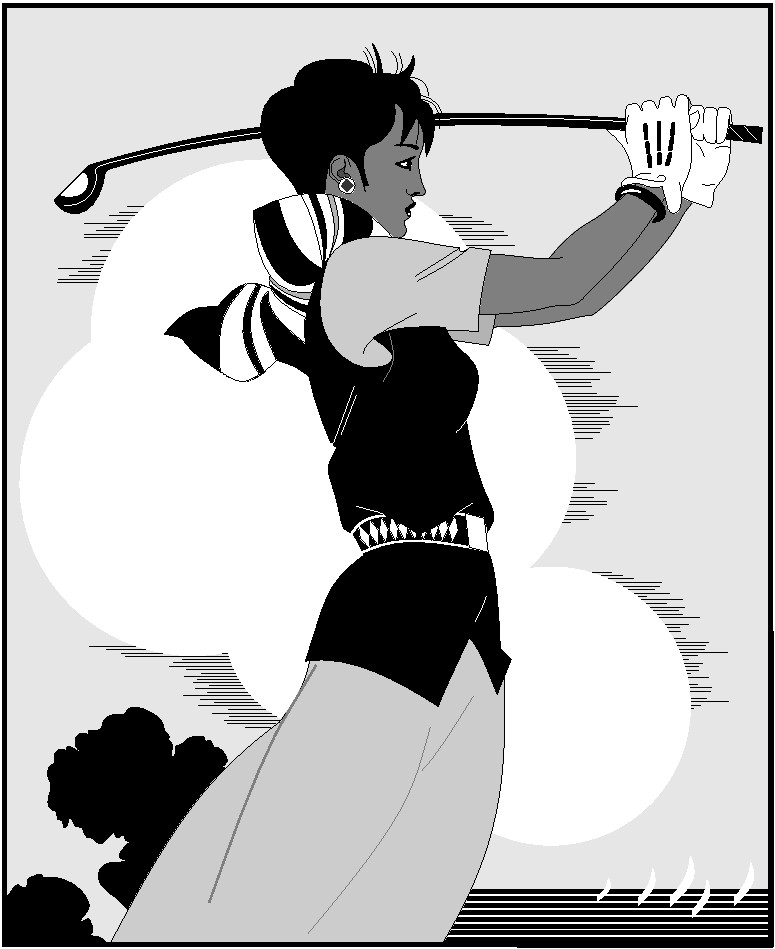
\includegraphics[width = 0.4\textwidth]{golfer}
% \bicaption[golfer1]{}{注意图中文字尽量用五号字
% }{Fig.$\!$}{The person playing golf}
% \end{figure}
% \end{latex}
% 单张单图题的格式如下,
% \begin{latex}
% \begin{figure}[h]
% \centering
% 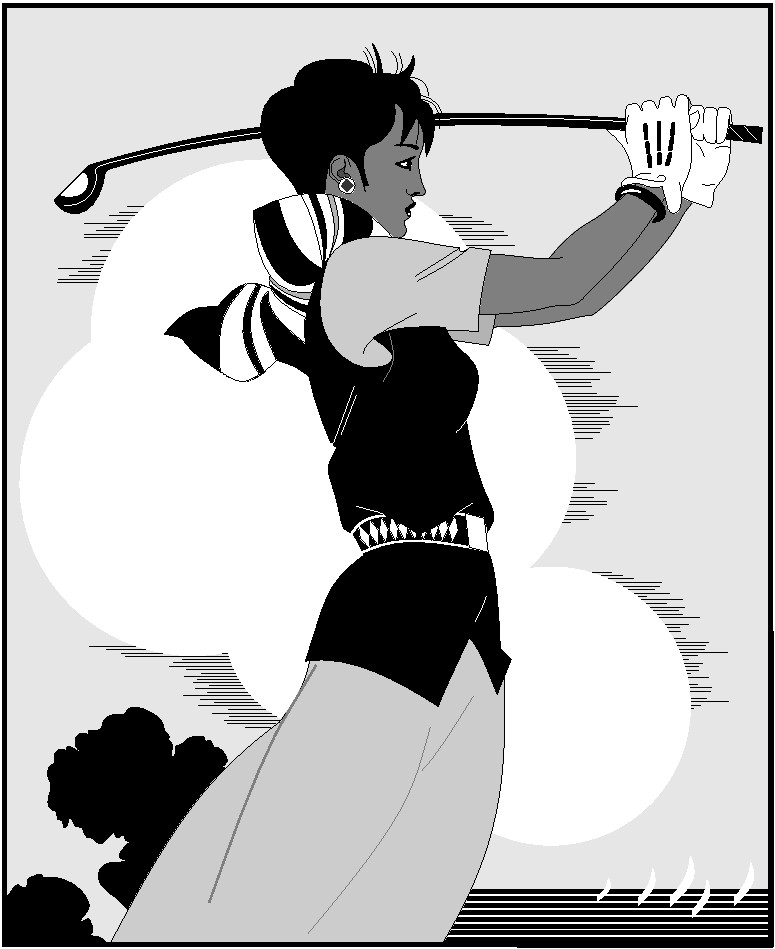
\includegraphics[width = 0.4\textwidth]{golfer}
% \caption{注意图中文字字号尽量用五号字}
% \end{figure}
% \end{latex}
% 并排图例。
% \begin{latex}
% \begin{figure}[htbp]
% \centering
% \begin{minipage}{0.4\textwidth}
% \centering
% 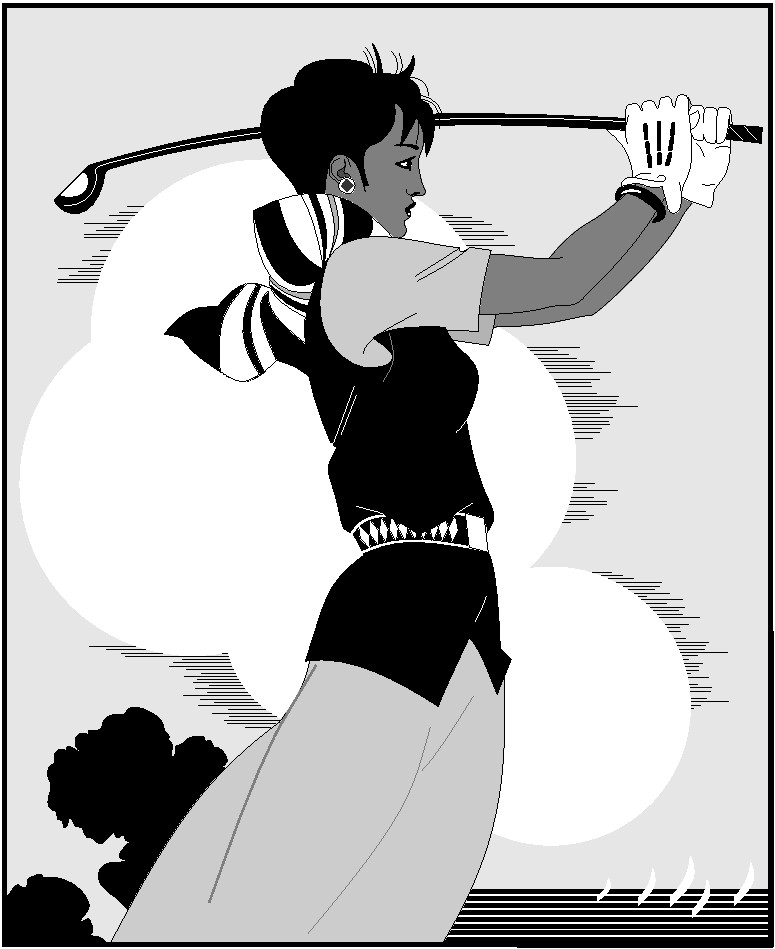
\includegraphics[width=\textwidth]{golfer}
% \bicaption[golfer2]{}{打高尔夫球的人}{Fig.$\!$}{The person playing golf}
% \end{minipage}
% \begin{minipage}{0.4\textwidth}
% \centering
% 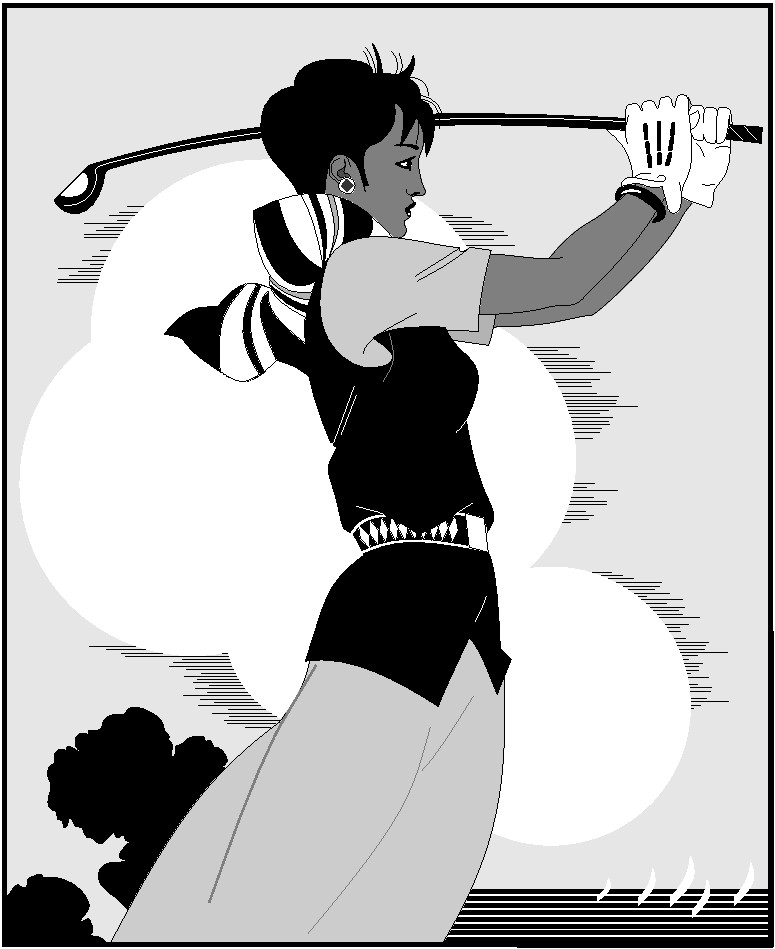
\includegraphics[width=\textwidth]{golfer}
% \bicaption[golfer3]{}{打高尔夫球的人}{Fig.$\!$}{The person playing golf}
% \end{minipage}
% \end{figure}
% \end{latex}
% 子图图例。
% \begin{latex}
% \begin{figure}[htbp]
% \centering
% \subfigure{\label{golfer41}}\addtocounter{subfigure}{-2}
% \subfigure[The person playing golf]{\subfigure[打高尔夫球的人~1]{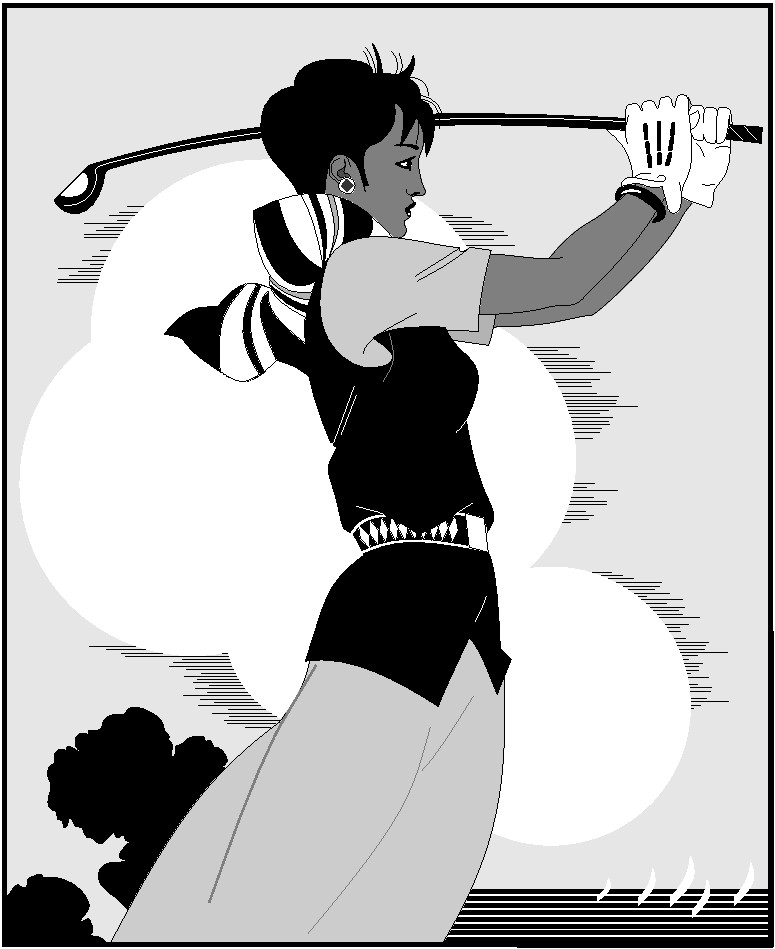
\includegraphics[width=0.4\textwidth]{golfer}}}
% \subfigure{\label{golfer42}}\addtocounter{subfigure}{-2}
% \subfigure[The person playing golf]{\subfigure[打高尔夫球的人~2]{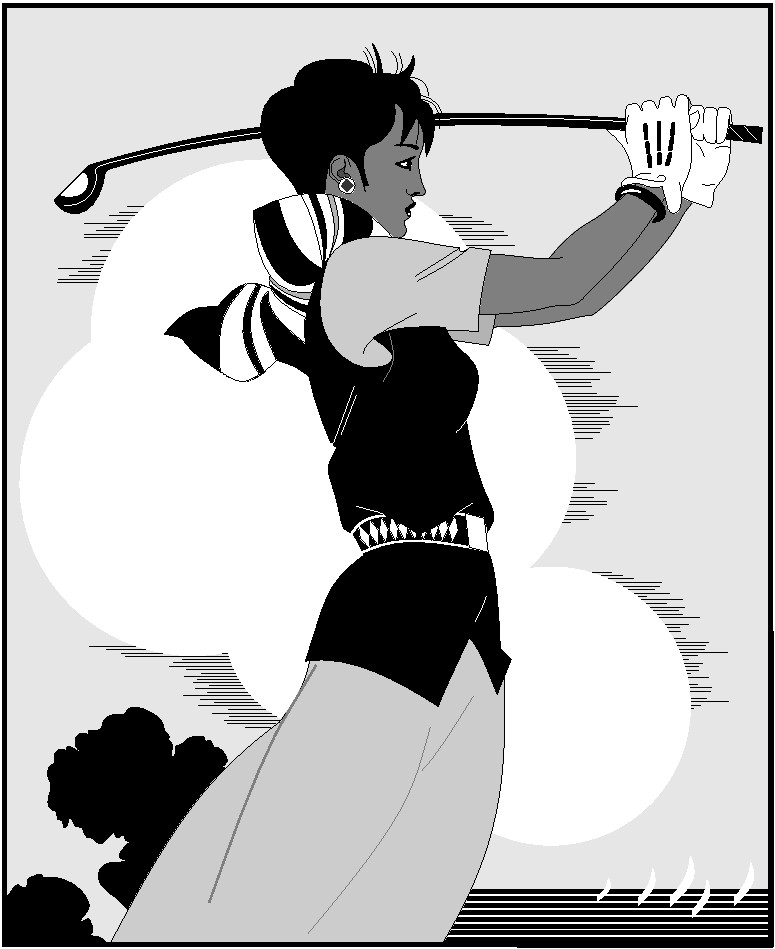
\includegraphics[width=0.4\textwidth]{golfer}}}
% \bicaption[golfer4]{}{打高尔夫球的人}{Fig.$\!$}{The person playing golf}
% \end{figure}
% \end{latex}
% 表格示例,表格中的字体是可以自行调整的。
% \begin{latex}
% \begin{table}[htbp]
% \bicaption[table1]{}{符合研究生院绘图规范的表格}{Table$\!$}{Table in agreement of the standard from graduate school}
% \vspace{0.5em}\centering\wuhao
% \begin{tabular}{ccccc}
% \toprule[1.5pt]
% $D$(in) & $P_u$(lbs) & $u_u$(in) & $\beta$ & $G_f$(psi.in)\\
% \midrule[1pt]
%  5 & 269.8 & 0.000674 & 1.79 & 0.04089\\
% 10 & 421.0 & 0.001035 & 3.59 & 0.04089\\
% 20 & 640.2 & 0.001565 & 7.18 & 0.04089\\
% \bottomrule[1.5pt]
% \end{tabular}
% \end{table}
% \end{latex}
% 因为长表格不是浮动体,不会自动调整位置、也不会自动调整字体大小,一切都要手动设
% 置。设置起来特别繁琐,建议尽量不要使用长表格。
% \begin{latex}
% \ltfontsize{\dawu[1.667]} %设置表格内字体行间距
% \dawu[1.667]\begin{longtable}{ccc} % 注意此处设置的是表格线距离
% \longbionenumcaption{}{{\wuhao 中国省级行政单位一览 %此处要添加字体设置
% }\label{table2}}{Table$\!$}{}{{\wuhao Overview of the provincial administrative
% unit of China}}{-0.5em}{3.15bp}\\ %注意后两个参数分别是中英标题间距、标题和表格的间距。
% %\caption{\wuhao 中国省级行政单位一览}\\[1em] %注意此处是标题和表格间距,这行
% %是单语标题
% \toprule[1.5pt] 名称 & 简称 & 省会或首府  \\ \midrule[1pt]
% \endfirsthead
% \multicolumn{3}{r}{表~\thetable(续表)}\vspace{0.5em}\\
% \toprule[1.5pt] 名称 & 简称 & 省会或首府  \\ \midrule[1pt]
% \endhead
% \bottomrule[1.5pt]
% \endfoot
% 北京市 & 京 & 北京\\
% 天津市 & 津 & 天津\\
% 河北省 & 冀 & 石家庄市\\
% 山西省 & 晋 & 太原市\\
% 内蒙古自治区 & 蒙 & 呼和浩特市\\
% 辽宁省 & 辽 & 沈阳市\\
% 吉林省 & 吉 & 长春市\\
% 黑龙江省 & 黑 & 哈尔滨市\\
% 上海市 & 沪/申 & 上海\\
% 江苏省 & 苏 & 南京市\\
% 浙江省 & 浙 & 杭州市\\
% 安徽省 & 皖 & 合肥市\\
% 福建省 & 闽 & 福州市\\
% 江西省 & 赣 & 南昌市\\
% 山东省 & 鲁 & 济南市\\
% 河南省 & 豫 & 郑州市\\
% 湖北省 & 鄂 & 武汉市\\
% 湖南省 & 湘 & 长沙市\\
% 广东省 & 粤 & 广州市\\
% 广西壮族自治区 & 桂 & 南宁市\\
% 海南省 & 琼 & 海口市\\
% 重庆市 & 渝 & 重庆\\
% 四川省 & 川/蜀 & 成都市\\
% 贵州省 & 黔/贵 & 贵阳市\\
% 云南省 & 云/滇 & 昆明市\\
% 西藏自治区 & 藏 & 拉萨市\\
% 陕西省 & 陕/秦 & 西安市\\
% 甘肃省 & 甘/陇 & 兰州市\\
% 青海省 & 青 & 西宁市\\
% 宁夏回族自治区 & 宁 & 银川市\\
% 新疆维吾尔自治区 & 新 & 乌鲁木齐市\\
% 香港特别行政区 & 港 & 香港\\
% 澳门特别行政区 & 澳 & 澳门\\
% 台湾省 & 台 & 台北市\\
% \end{longtable}\normalsize %注意这里要恢复正常字体
% \end{latex}
%
% \subsubsection{公式}
% 公式不做介绍,与正常用法一致。
%
% \subsubsection{数学环境}
% \label{sec:math}
% \heuthesis\ 定义了常用的数学环境:
%
% \begin{center}
% \begin{tabular}{*{7}{l}}\toprule
%   axiom & theorem & definition & proposition & lemma & conjecture &\\
%   公理 & 定理 & 定义 & 命题 & 引理 & 猜想 &\\\midrule
%   proof & corollary & example & exercise & assumption & remark & problem \\
%   证明 & 推论 & 例子& 练习 & 假设 & 注释 & 问题\\\bottomrule
% \end{tabular}
% \end{center}
%
% 比如:
% \begin{latex}
% \begin{definition}
%   道千乘之国,敬事而信,节用而爱人,使民以时。
% \end{definition}
% \end{latex}
% 产生(自动编号):
% \medskip
%
% \noindent\framebox[\linewidth][l]{{\heiti 定义~1.1~~~} % {道千乘之国,敬事而信,节用而爱人,使民以时。}}
%
% \smallskip
% 列举出来的数学环境毕竟是有限的,如果想用\emph{胡说}这样的数学环境,那么可以定义:
% \begin{latex}
% \newtheorem{nonsense}{胡说}[chapter]
% \end{latex}
%
% 然后这样使用:
% \begin{latex}
% \begin{nonsense}
%   契丹武士要来中原夺武林秘笈。—— 慕容博
% \end{nonsense}
% \end{latex}
% 产生(自动编号):
%
% \medskip
% \noindent\framebox[\linewidth][l]{{\heiti 胡说~1.1~~~} % {契丹武士要来中原夺武林秘笈。—— 慕容博}}
%
% \subsubsection{算法}
% 我校算法不在规范中要求,且每个人都有自己的算法格式喜好,大家最好采用大家普遍接收的方式,做到美观、协调就可以。
%
% \subsubsection{引用参考文献}
% \DescribeMacro{\inlinecite}
% 学校要求的参考文献引用有两种模式:(1)上标模式。比如``同样的工作有很
% 多$^{[1,2]}$\ldots''。(2)正文模式。比如``文[3] 中详细说明了\ldots''。其中上标
% 模式使用远比正文模式频繁,所以为了符合使用习惯,上标模式仍然用常规
% 的 \cs{cite}\marg{key},而 \cs{inlinecite}\marg{key} 则用来生成正文模式。
%
% 关于参考文献模板推荐使用 \BibTeX,关于中文参考文献需要额外增加一个 Entry:
% \texttt{language},将其设置为 \texttt{zh} 用来指示此参考文献为中文,以
% 便 \file{heuthesis.bst} 处理。如:
% \begin{latex}
% @INPROCEEDINGS{cnproceed,
%   author    = {王重阳 and 黄药师 and 欧阳峰 and 洪七公 and 段皇帝},
%   title     = {武林高手从入门到精通},
%   booktitle = {第~$N$~次华山论剑},
%   year      = 2006,
%   address   = {西安, 中国},
%   month     = sep,
%   language  = "zh",
% }
%
% @ARTICLE{cnarticle,
%   AUTHOR  = "贾宝玉 and 林黛玉 and 薛宝钗 and 贾探春",
%   TITLE   = "论刘姥姥食量大如牛之现实意义",
%   JOURNAL = "红楼梦杂谈",
%   PAGES   = "260--266",
%   VOLUME  = "224",
%   YEAR    = "1800",
%   LANGUAGE= "zh",
% }
% \end{latex}
%
% 注意如果不需要引用参考文献,请删除 \file{main.tex} 中 \cs{bibliography} 开头的两行,
% 以避免可能的编译错误。
%
% \subsubsection{列表环境}
% \DescribeEnv{itemize}
% \DescribeEnv{enumerate}
% \DescribeEnv{description}
% 为了适合中文习惯,模板将这三个常用的列表环境用 \pkg{enumitem} 进行了纵向间距压
% 缩。一方面清除了多余空间,另一方面用户可以自己指定列表环境的样式(如标签符号,
% 缩进等)。细节请参看 \pkg{enumitem} 文档,此处不再赘述。
% \subsection{后文}
%
% \subsubsection{结论}
% \DescribeEnv{conclusion}
% 结论之后为后文内容。
% \begin{latex}
% \begin{conclusions}
%
% 学位论文的结论作为论文正文的最后一章单独排写,但不加章标题序号。
%
% 结论应是作者在学位论文研究过程中所取得的创新性成果的概要总结,不能与摘要混为一
% 谈。博士学位论文结论应包括论文的主要结果、创新点、展望三部分,在结论中应概括论
% 文的核心观点,明确、客观地指出本研究内容的创新性成果(含新见解、新观点、方法创
% 新、技术创新、理论创新),并指出今后进一步在本研究方向进行研究工作的展望与设想
% 。对所取得的创新性成果应注意从定性和定量两方面给出科学、准确的评价,分(1)、
% (2)、(3)…条列出,宜用“提出了”、“建立了”等词叙述。
%
% \end{conclusions}
% \end{latex}
%
% \subsubsection{参考文献}
% 在后文中的参考文献是自动生成的,不需要用户干预,具体命令在\file{main.tex}中有
% 示例。
%
% \subsubsection{附录}
% \DescribeEnv{appendix}
% 所有的附录都插到这里来。因为附录会更改默认的 chapter 属性,而后面的{\heiti 个人简
%   历}又需要恢复,所以实现为环境可以保证全局的属性不受影响。
% \begin{latex}
% \begin{appendix}
% % -*-coding: utf-8 -*-
%%%%%%%%%%%%%%%%%%%%%%%%%%%%%%%%%%%%%%%%%%%%%%%%%%%%%%%%%
\chapter{带章节的附录}[Full Appendix]%
完整的附录内容,包含章节,公式,图表等

%%%%%%%%%%%%%%%%%%%%%%%%%%%%%%%%%%%%%%%%%%%%%%%%%%%%%%%%%
\section{附录节的内容}[Section in Appendix]
这是附录的节的内容

附录中图的示例:
\begin{figure}[htbp]
\centering
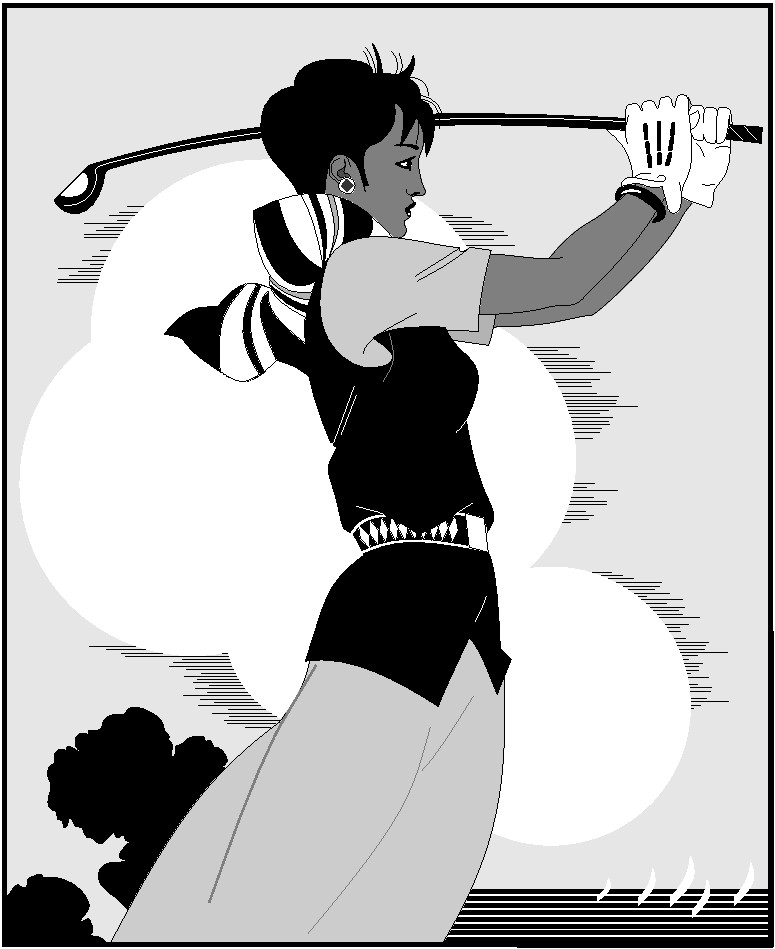
\includegraphics[width = 0.4\textwidth]{golfer}
%\bicaption[golfer5]{}{\xiaosi[0]打高尔夫球的人}{Fig.$\!$}{The person playing golf}\vspace{-1em}
\caption{\xiaosi[0]打高尔夫球的人}
\end{figure}

附录中公式的示例:
\begin{align}
a & = b \times c \\
E & = m c^2
\label{eq}
\end{align}

\chapter{这个星球上最好的免费Linux软件列表}[List of the Best Linux Software in our Planet]
\section{系统}

\href{http://fvwm.org/}{FVWM自从上世纪诞生以来,此星球最强大的窗口管理器。}
推荐基于FVWM的桌面设计hifvwm:\href{https://github.com/dustincys/hifvwm}{https://github.com/dustincys/hifvwm}。

\subsection{hifvwm的优点}

\begin{enumerate}
	\item 即使打开上百个窗口也不会“蒙圈”,对比win或mac都无法做到。计算机性能越来越强大,窗口任务的管理必须要升级到打怪兽级别。
	\item 二维可视化任务栏。
	\item 自动同步Bing搜索主页的壁纸。每次电脑开机,午夜零点自动更新,用户
		也可以手动更新,从此审美再也不疲劳。
	\item 切换窗口自动聚焦到最上面的窗口。使用键盘快捷键切换窗口时候,减少
		操作过程,自动聚焦到目标窗口。这一特性是虚拟窗口必须的人性化设
		计。
	\item 类似window右下角的功能的最小化窗口来显示桌面的功能此处类似
		win7/win10,实现在一个桌面之内操作多个任务。
	\item 任务栏结合标题栏。采用任务栏和标题栏结合,节省空间。
	\item 同类窗口切换。可以在同类窗口之内类似alt-tab的方式切换。
	\item ……
\end{enumerate}

\section{其他}

\href{https://github.com/goldendict/goldendict}{goldendict 星球最强大的桌面字典。}

\href{https://github.com/yarrick/iodine}{iodine,“HIT-WLAN + 锐捷”时代的福音。}

\href{http://www.aircrack-ng.org/}{aircrack,Wifi“安全性评估”工具,自由上网,
  就是隔壁寝室网络会变慢一点。}

\href{https://www.ledger-cli.org/}{ledger,前“金融区块链”时代最好的复式记账系统。}

\href{https://orgmode.org/}{orgmode,最强大的笔记系统,从来没有之一。}

\href{https://www.jianguoyun.com/}{坚果云,国内一款支持WebDav的云盘系统,国内真正的云盘没有之一。}

\href{https://notmuchmail.org/}{notmuch, 目前最好的邮件管理工具,还在为每天几百
  个email苦恼?几百个这些都不算多,notmuch。}

\section{vim}
实现中英文每一句一行,以及实现每一句折叠断行的简单正则式,tex源码更加乖乖。
\begin{lstlisting}
vnoremap <leader>fae J:s/[.!?]\zs\s\+/\="\r".matchstr(getline('.'), '^\s*')/g<CR>
vnoremap <leader>fac J:s/[。!?]/\=submatch(0)."\n".matchstr(getline('.'), '^\s*')/g<CR>
vnoremap <leader>fle :!fmt -80 -s<CR>
\end{lstlisting}

% \end{appendix}
% \end{latex}
%
% \subsubsection{所发表文章}
% \DescribeEnv{publication}
% 虽然在\PGR\UGR\ 中都没有明确规定此处的格式,
% 此处基本按照参考文献的要求进行设置。
% \begin{latex}
% \begin{publication}
% \noindent\textbf{(一)发表的学术论文}
% \begin{publist}
% \item XXX,XXX. Static Oxidation Model of Al-Mg/C Dissipation Thermal Protection Materials[J]. Rare Metal Materials and Engineering, 2010, 39(Suppl. 1): 520-524.(SCI~收录,IDS号为~669JS,IF=0.16)
% \item XXX,XXX. 精密超声振动切削单晶铜的计算机仿真研究[J]. 系统仿真学报,2007,19(4):738-741,753.(EI~收录号:20071310514841)
% \item XXX,XXX. 局部多孔质气体静压轴向轴承静态特性的数值求解[J]. 摩擦学学报,2007(1):68-72.(EI~收录号:20071510544816)
% \item XXX,XXX. 硬脆光学晶体材料超精密切削理论研究综述[J]. 机械工程学报,2003,39(8):15-22.(EI~收录号:2004088028875)
% \item XXX,XXX. 基于遗传算法的超精密切削加工表面粗糙度预测模型的参数辨识以及切削参数优化[J]. 机械工程学报,2005,41(11):158-162.(EI~收录号:2006039650087)
% \item XXX,XXX. Discrete Sliding Mode Cintrok with Fuzzy Adaptive Reaching Law on 6-PEES Parallel Robot[C]. Intelligent System Design and Applications, Jinan, 2006: 649-652.(EI~收录号:20073210746529)
% \end{publist}
%
% \noindent\textbf{(二)申请及已获得的专利(无专利时此项不必列出)}
% \begin{publist}
% \item XXX,XXX. 一种温热外敷药制备方案:中国,88105607.3[P]. 1989-07-26.
% \end{publist}
%
% \noindent\textbf{(三)参与的科研项目及获奖情况}
% \begin{publist}
% \item XXX,XXX. XX~气体静压轴承技术研究, XX~省自然科学基金项目.课题编号:XXXX.
% \item XXX,XXX. XX~静载下预应力混凝土房屋结构设计统一理论. 黑江省科学技术二等奖, 2007.
% \end{publist}
% %\vfill
% %\hangafter=1\hangindent=2em\noindent
% %\setlength{\parindent}{2em}
% \end{publication}
% \end{latex}
%
% \subsubsection{索引}
% \DescribeEnv{ceindex}
% 我校要求中英文双语索引。后文中的自动索引实际上不需要用户干预。
%\begin{latex}
% \begin{ceindex}
%   %如果想要手动加索引,注释掉以下这一样,用wordlist环境
% \printsubindex*
% \end{ceindex}
%\end{latex}
% 手工添加索引的方法不推荐,模板中将去除该功能。
%
% \subsubsection{致谢声明}
% \DescribeEnv{acknowledgement}
% 把致谢做成一个环境更好一些,直接往里面写感谢的话就可以啦!
%
% \begin{latex}
% \begin{acknowledgement}
%   …
%   感谢哈尔滨工程大学\ \LaTeX\ 论文模板\heuthesis\ !
% \end{acknowledgement}
% \end{latex}
%
%
% \subsubsection{简历}
% \DescribeEnv{resume}
% 个人简历。
% 实际上,致谢和个人简历是自由发挥的地区,字体,文体,格式,内容,完全自己决定。
% \begin{latex}
% \begin{resume}
% XXXX~年~XX~月~XX~日出生于~XXXX。
%
% XXXX~年~XX~月考入~XX~大学~XX~院(系)XX~专业,XXXX~年~XX~月本科毕业并获得~XX~学学士学位。
%
% XXXX~年~XX~月------XXXX~年~XX~月在~XX~大学~XX~院(系)XX~学科学习并获得~XX~学硕士学位。
%
% XXXX~年~XX~月------XXXX~年~XX~月在~XX~大学~XX~院(系)XX~学科学习并获得~XX~学博士学位。
%
% 获奖情况:如获三好学生、优秀团干部、X~奖学金等(不含科研学术获奖)。
%
% 工作经历:
% \end{resume}
% \end{latex}
%
% \subsubsection{授权}
% \DescribeMacro{\authorization}
% 授权页中的签名和日期是需要手写,不需要人工干预。
% 模板中提供了未签名的空白论文原创性声明和授权页 \file{authorization.pdf},
% 可以使用签字后的扫描版文件进行替换。
%\begin{latex}
% \authorization[authorization.pdf]
%\end{latex}
%
% \subsection{其它}
% 模板的配置文件 \file{heuthesisbook.cfg} 中定义了很多固定词汇,一般无须修改。如果有特殊需求,
% 推荐在导言区使用 \cs{renewcommand}。
%
%
% \StopEventually{\PrintChanges\PrintIndex}
% \clearpage
%
% \section{实现细节}
%
% \subsection{基本信息}
% \changes{v1.0.0}{2021/11/11}{移植自hitThesis论文模板}
%    \begin{macrocode}
%<*bst>
ENTRY                                             % class Entry {
{                                                 % public:
  author                                          %   String author;
  editor                                          %   String editor;
  translator                                      %   String translator;
  title                                           %   String title;
  edition                                         %   String edition;
  address                                         %   String address;
  publisher                                       %   String publisher;
  pages                                           %   String pages;
  year                                            %   String year;
  date                                            %   String date;
  modifydate                                      %   String modifydate;
  citedate                                        %   String citedate;
  url                                             %   String url;
  doi                                             %   String doi;
  language                                        %   String language;
  booktitle                                       %   String booktitle;
  journal                                         %   String journal;
  chapter                                         %   String chapter;
  series                                          %   String series;
  volume                                          %   String volume;
  number                                          %   String number;
  version                                         %   String version;
  month                                           %   String month;
  school                                          %   String school;
  institution                                     %   String institution;
  organization                                    %   String organization;
  type                                            %   String type;
  howpublished                                    %   String howpublished;
  eid                                             %   String eid;
  key                                             %   String key;
  country                                         %   String country;
  patentid                                        %   String patentid;
  media                                           %   String media;
} {                                               %   //  declare integer variables
  required                                        %   int required;  // withther the bibfield is required
} {                                               %   //  declare String variables
  label                                           %   String label;           //  label for the entry
  mark                                            %   String mark;            //  mark for the entry
                                                  %   //  there is ahidden entry variable sort.key$
                                                  %   String sort_key;
}                                                 % }
                                                  %
%%%%%%%%%%%%%%%%%%%%%%%%%%%%%%%%%%%%%%%%%%%%%%%%%%%%%%%%%%%%%%%%%%%%%%%%%%%%%%%
                                                  %
INTEGERS {                                        % //  declare global int variables
  entry.count                                     % static int entry_count;          // number of entries
  longest.label.width                             % static int longest_label_width;  // width of the longest label
  i                                               % static int i;
  j                                               % static int j;
  k                                               % static int k;
}                                                 %
                                                  %
%%%%%%%%%%%%%%%%%%%%%%%%%%%%%%%%%%%%%%%%%%%%%%%%%%%%%%%%%%%%%%%%%%%%%%%%%%%%%%%
                                                  %
STRINGS {                                         % //  declare global String variables
  longest.label                                   % static String longest_label;     //  the longest label
  s                                               % static String s;
  t                                               % static String t;
}                                                 %
                                                  %
%%%%%%%%%%%%%%%%%%%%%%%%%%%%%%%%%%%%%%%%%%%%%%%%%%%%%%%%%%%%%%%%%%%%%%%%%%%%%%%

% define global static constants
FUNCTION {true}                 {#1}
FUNCTION {false}                {#0}
FUNCTION {debug.enabled}        {true}
FUNCTION {cap.volume.en}        {"Vol~"}
FUNCTION {cap.volume.zh}        {"卷"}
FUNCTION {cap.edition.en}       {"~ed"}
FUNCTION {cap.edition.zh}       {"版"}
FUNCTION {cap.anonymous.en}     {"Anon"}
FUNCTION {cap.anonymous.zh}     {"佚名"}
FUNCTION {cap.no.address.en}    {"[S.l.]"}
FUNCTION {cap.no.address.zh}    {"[出版地不详]"}
FUNCTION {cap.no.publisher.en}  {"[s.n.]"}
FUNCTION {cap.no.publisher.zh}  {"[出版者不详]"}
FUNCTION {cap.et.al.en}         {", et~al"}
FUNCTION {cap.et.al.zh}         {", 等"}
FUNCTION {cap.translate.en}     {"~trans"}
FUNCTION {cap.translate.zh}     {"译"}
FUNCTION {cap.doi.url}          {"http://dx.doi.org/"}
FUNCTION {cap.st.en}            {"st"}
FUNCTION {cap.nd.en}            {"nd"}
FUNCTION {cap.rd.en}            {"rd"}
FUNCTION {cap.th.en}            {"th"}

FUNCTION {cap.space}            {" "}
FUNCTION {cap.period}           {"\@. "}
FUNCTION {cap.comma}            {"\@, "}
FUNCTION {cap.colon}            {"\textnormal{: }"}
FUNCTION {cap.double.slash}     {" //\thinspace{}"}
FUNCTION {cap.dash}             {"\textnormal{-}"}

% Predefined latex command used to format the style of bibitems
FUNCTION {env.bibbegin}         { "\begin{thebibliography}" }
FUNCTION {env.bibend}           { "\end{thebibliography}" }
FUNCTION {cmd.bibauthor}        { "\providecommand{\bibauthor}[1]{#1}" }
FUNCTION {cmd.bibeditor}        { "\providecommand{\bibeditor}[1]{#1}" }
FUNCTION {cmd.bibtranslator}    { "\providecommand{\bibtranslator}[1]{#1}" }
FUNCTION {cmd.bibtitle}         { "\providecommand{\bibtitle}[1]{#1}" }
FUNCTION {cmd.bibbooktitle}     { "\providecommand{\bibbooktitle}[1]{#1}" }
FUNCTION {cmd.bibjournal}       { "\providecommand{\bibjournal}[1]{#1}" }
FUNCTION {cmd.bibmark}          { "\providecommand{\bibmark}[1]{\mbox{#1}}" }
FUNCTION {cmd.bibcountry}       { "\providecommand{\bibcountry}[1]{#1}" }
FUNCTION {cmd.bibpatentid}      { "\providecommand{\bibpatentid}[1]{#1}" }
FUNCTION {cmd.bibedition}       { "\providecommand{\bibedition}[1]{#1}" }
FUNCTION {cmd.biborganization}  { "\providecommand{\biborganization}[1]{#1}" }
FUNCTION {cmd.bibaddress}       { "\providecommand{\bibaddress}[1]{#1}" }
FUNCTION {cmd.bibpublisher}     { "\providecommand{\bibpublisher}[1]{#1}" }
FUNCTION {cmd.bibinstitution}   { "\providecommand{\bibinstitution}[1]{#1}" }
FUNCTION {cmd.bibschool}        { "\providecommand{\bibschool}[1]{#1}" }
FUNCTION {cmd.bibvolume}        { "\providecommand{\bibvolume}[1]{#1}" }
FUNCTION {cmd.bibnumber}        { "\providecommand{\bibnumber}[1]{#1}" }
FUNCTION {cmd.bibversion}       { "\providecommand{\bibversion}[1]{#1}" }
FUNCTION {cmd.bibpages}         { "\providecommand{\bibpages}[1]{#1}" }
FUNCTION {cmd.bibmodifydate}    { "\providecommand{\bibmodifydate}[1]{#1}" }
FUNCTION {cmd.bibcitedate}      { "\providecommand{\bibcitedate}[1]{#1}" }
FUNCTION {cmd.bibyear}          { "\providecommand{\bibyear}[1]{#1}" }
FUNCTION {cmd.bibdate}          { "\providecommand{\bibdate}[1]{#1}" }
FUNCTION {cmd.biburl}           { "\providecommand{\biburl}[1]{\newline\url{#1}}" }

%%%%%%%%%%%%%%%%%%%%%%%%%%%%%%%%%%%%%%%%%%%%%%%%%%%%%%%%%%%%%%%%%%%%%%%%%%%%%%%
                                                  %
FUNCTION {log.str} {                              % void Entry::log_str(String value, String message)
  debug.enabled {                                 %   if (debug_enabled == 1) {
    "DEBUG: " swap$ * " - '" *                    %     message = "DEBUG: " + message + " - '";
    swap$ *                                       %     message = message + value;
    "'" *                                         %     message = message + "'";
    top$                                          %     log(message);
  } {                                             %   } else {
    pop$ pop$                                     %     return;
  } if$                                           %   }
}                                                 % }
                                                  %
%%%%%%%%%%%%%%%%%%%%%%%%%%%%%%%%%%%%%%%%%%%%%%%%%%%%%%%%%%%%%%%%%%%%%%%%%%%%%%%
                                                  %
FUNCTION {log.int} {                              % int Entry::log_int(int value, String message)
  debug.enabled {                                 %   if (debug_enabled == 1) {
    "DEBUG: " swap$ * " - " *                     %     message = "DEBUG: " + message + " - ";
    swap$ int.to.str$ *                           %     message = message + int_to_str(value);
    top$                                          %     log(message);
  } {                                             %   } else {
    pop$ pop$                                     %     return;
  } if$                                           %   }
}                                                 % }
                                                  %
%%%%%%%%%%%%%%%%%%%%%%%%%%%%%%%%%%%%%%%%%%%%%%%%%%%%%%%%%%%%%%%%%%%%%%%%%%%%%%%
                                                  %
FUNCTION {not} {                                  % int Entry::not(int x) {
  {                                               %   if (x == 1) {
    false                                         %     return false;
  } {                                             %   } else {
    true                                          %     return true;
  } if$                                           %   }
}                                                 % }
                                                  %
%%%%%%%%%%%%%%%%%%%%%%%%%%%%%%%%%%%%%%%%%%%%%%%%%%%%%%%%%%%%%%%%%%%%%%%%%%%%%%%
                                                  %
FUNCTION {and} {                                  % int Entry::and(int x, int y) {
  {                                               %   if (y == 1) {
    skip$                                         %     return x;
  } {                                             %   } else {
    pop$ false                                    %     return false;
  } if$                                           %   }
}                                                 % }
                                                  %
%%%%%%%%%%%%%%%%%%%%%%%%%%%%%%%%%%%%%%%%%%%%%%%%%%%%%%%%%%%%%%%%%%%%%%%%%%%%%%%
                                                  %
FUNCTION {or} {                                   % int Entry::or(int x, int y) {
  {                                               %   if (y == 1) {
    pop$ true                                     %     return true;
  } {                                             %   } else {
    skip$                                         %     return x;
  } if$                                           %   }
}                                                 % }
                                                  %
%%%%%%%%%%%%%%%%%%%%%%%%%%%%%%%%%%%%%%%%%%%%%%%%%%%%%%%%%%%%%%%%%%%%%%%%%%%%%%%
                                                  % //  calculate the length in characters of a string
                                                  % //  We need this function since text.length$ is NOT
                                                  % //  the length in characters.
INTEGERS {length.i}                               % static int length_i;
FUNCTION {length} {                               % int Entry::length(String str) {
  duplicate$ empty$ {                             %   if (empty(str)) {
    pop$ #0                                       %     return 0;
  } {                                             %   } else {
    #1 'length.i :=                               %     length_i = 1;
    false                                         %     int stop = false;
    {not} {                                       %     while (! stop) {
      duplicate$ length.i #1 substring$           %       String tmp = substring(str, length_i, 1);
      "" = {                                      %       if (tmp == "") {
        true                                      %         stop = true;
      } {                                         %       } else {
        length.i #1 + 'length.i :=                %         length_i = length_i + 1;
        false                                     %         stop = false;
      } if$                                       %       }
    } while$                                      %     }
    pop$ length.i #1 -                            %     return length_i - 1;
  } if$                                           %   }
}                                                 % }
                                                  %
%%%%%%%%%%%%%%%%%%%%%%%%%%%%%%%%%%%%%%%%%%%%%%%%%%%%%%%%%%%%%%%%%%%%%%%%%%%%%%%
                                                  %
FUNCTION {is.digit} {                             % int Entry::is_digit(String ch) {
  chr.to.int$                                     %   int ascii = chr_to_int(ch);
  duplicate$ "0" chr.to.int$ < {                  %   if (ascii < chr_to_int("0")) {
    pop$ false                                    %     return false;
  } {                                             %   } else {
    "9" chr.to.int$ > {                           %     if (ascii > chr_to_int("9")) {
      false                                       %       return false;
    } {                                           %     } else {
      true                                        %       return true;
    } if$                                         %     }
  } if$                                           %   }
}                                                 % }
                                                  %
%%%%%%%%%%%%%%%%%%%%%%%%%%%%%%%%%%%%%%%%%%%%%%%%%%%%%%%%%%%%%%%%%%%%%%%%%%%%%%%
                                                  % // test if str is a number
FUNCTION {is.number} {                            % int Entry::is_number(String str) {
  duplicate$ empty$ not swap$                     %   int result = (! empty(str));
  { duplicate$ empty$ not} {                      %   while (! empty(str)) {
    duplicate$ #1 #1 substring$ is.digit {        %     if (is_digit(substring(str, 1, 1))) {
      #2 global.max$ substring$                   %       str = substring(str, 2, global_max);
    } {                                           %     } else {
      pop$ pop$ false                             %       result = false;
      ""                                          %       str = "";
    } if$                                         %     }
  } while$                                        %   }
  pop$                                            %   return result;
}                                                 % }
                                                  %
%%%%%%%%%%%%%%%%%%%%%%%%%%%%%%%%%%%%%%%%%%%%%%%%%%%%%%%%%%%%%%%%%%%%%%%%%%%%%%%
                                                  % // extract the number prefix of str
FUNCTION {extract.number} {                       % String Entry::extract_number(String str) {
  duplicate$                                      %   String suffix = str;
  duplicate$ length swap$                         %   int n = length(str);
  duplicate$ empty$                               %   int stop = empty(suffix);
  { not } {                                       %   while (! stop) {
    duplicate$ #1 #1 substring$ is.digit {        %     if (is_digit(substring(suffix, 1, 1))) {
      #2 global.max$ substring$                   %       suffix = substring(suffix, 2, global_max);
      duplicate$ empty$                           %       stop = empty(suffix);
    } {                                           %     } else {
      true                                        %       stop = true;
    } if$                                         %     }
  } while$                                        %   }
  length -                                        %   int n = n - length(suffix);
  #1 swap$ substring$                             %   return substring(str, 1, n);
}                                                 % }
                                                  %
%%%%%%%%%%%%%%%%%%%%%%%%%%%%%%%%%%%%%%%%%%%%%%%%%%%%%%%%%%%%%%%%%%%%%%%%%%%%%%%
                                                  %
FUNCTION {get.last.chr} {                         % String Entry::get_last_chr(String str) {
  duplicate$ length                               %   int n = length(str);
  duplicate$ #0 = {                               %   if (n == 0) {
    pop$                                          %     return str;
  } {                                             %   } else {
    #1 substring$                                 %     return substring(str, n, 1);
  } if$                                           %   }
}                                                 % }
                                                  %
%%%%%%%%%%%%%%%%%%%%%%%%%%%%%%%%%%%%%%%%%%%%%%%%%%%%%%%%%%%%%%%%%%%%%%%%%%%%%%%
                                                  %
FUNCTION {get.ordinal.suffix.en} {                % String Entry::get_ordinal_suffix_en(String ch) {
  duplicate$ "1" = {                              %   if (num == "1") {
    pop$ cap.st.en                                %     return cap_st_en;
  } {                                             %   } else {
    duplicate$ "2" = {                            %     if (num == "2") {
      pop$ cap.nd.en                              %       return cap_nd_en;
    } {                                           %     } else {
      duplicate$ "3" = {                          %       if (num == "3") {
        pop$ cap.rd.en                            %         return cap_rd_en;
      } {                                         %       } else {
        pop$ cap.th.en                            %         return cap_th_en;
      } if$                                       %       }
    } if$                                         %     }
  } if$                                           %   }
}                                                 % }
                                                  %
%%%%%%%%%%%%%%%%%%%%%%%%%%%%%%%%%%%%%%%%%%%%%%%%%%%%%%%%%%%%%%%%%%%%%%%%%%%%%%%
                                                  %
FUNCTION {num.to.ordinal.en} {                    % String Entry::num_to_ordinal_en(String num) {
  duplicate$ empty$ {                             %   if (empty(num)) {
    skip$                                         %     return num;
  } {                                             %   } else {
    duplicate$ get.last.chr                       %     String ch = get_last_chr(num);
    get.ordinal.suffix.en                         %     String str = get_ordinal_suffix_en(ch);
    *                                             %     reutrn num + str;
  } if$                                           %   }
}                                                 % }
                                                  %
%%%%%%%%%%%%%%%%%%%%%%%%%%%%%%%%%%%%%%%%%%%%%%%%%%%%%%%%%%%%%%%%%%%%%%%%%%%%%%%
                                                  %
STRINGS {remove.dots.result}                      % static String remove_dots_result;
                                                  %
FUNCTION {remove.dots} {                          % String Entry::remove_dots(String str) {
  "" 'remove.dots.result :=                       %   remove_dots_result = "";
  { duplicate$ empty$ not } {                     %   while (! empty(str)) {
    duplicate$ #1 #2 substring$                   %     String tmp = substring(str, 1, 2);
    "\." = {                                      %     if (tmp == "\.") {
      #3 global.max$ substring$                   %       str = substring(str, 3, global_max);
    } {                                           %     } else {
      duplicate$ #1 #1 substring$                 %       tmp = substring(str, 1, 1);
      duplicate$ "." = {                          %       if (tmp == ".") {
        pop$ #2 global.max$ substring$            %         str = substring(str, 2, global_max);
      } {                                         %       } else {
        remove.dots.result swap$ *                %         tmp = remove_dots_result + tmp;
        'remove.dots.result :=                    %         remove_dots_result = tmp;
        #2 global.max$ substring$                 %         str = substring(str, 2, global_max);
      } if$                                       %       }
    } if$                                         %     }
  } while$                                        %   }
  pop$ remove.dots.result                         %   return remove_dots_result;
}                                                 % }
                                                  %
%%%%%%%%%%%%%%%%%%%%%%%%%%%%%%%%%%%%%%%%%%%%%%%%%%%%%%%%%%%%%%%%%%%%%%%%%%%%%%%
                                                  %
FUNCTION {add.brace} {                            % String Entry::add_brace(String str) {
  "{" swap$ * "}" *                               %   return "{" + str + "}";
}                                                 % }
                                                  %
%%%%%%%%%%%%%%%%%%%%%%%%%%%%%%%%%%%%%%%%%%%%%%%%%%%%%%%%%%%%%%%%%%%%%%%%%%%%%%%
                                                  %
FUNCTION {add.bracket} {                          % String Entry::bracket(String str) {
  "(" swap$ * ")" *                               %   return "(" + str + ")";
}                                                 % }
                                                  %
%%%%%%%%%%%%%%%%%%%%%%%%%%%%%%%%%%%%%%%%%%%%%%%%%%%%%%%%%%%%%%%%%%%%%%%%%%%%%%%
                                                  %
FUNCTION {add.squarebracket} {                    % String Entry::add_squarebracket(String str) {
  "[" swap$ * "]" *                               %   return "[" + str + "]";
}                                                 % }
                                                  %
%%%%%%%%%%%%%%%%%%%%%%%%%%%%%%%%%%%%%%%%%%%%%%%%%%%%%%%%%%%%%%%%%%%%%%%%%%%%%%%
                                                  %
FUNCTION {add.textit} {                           % String Entry::add_textit(String str) {
  "\textit{" swap$ * "}" *                        %   return "\textit{" + str + "}";
}                                                 % }
                                                  %
%%%%%%%%%%%%%%%%%%%%%%%%%%%%%%%%%%%%%%%%%%%%%%%%%%%%%%%%%%%%%%%%%%%%%%%%%%%%%%%
                                                  %
FUNCTION {add.textbf} {                           % String Entry::add_textbf(String str) {
  "\textbf{" swap$ * "}" *                        %   return "\textbf{" + str + "}";
}                                                 % }
                                                  %
%%%%%%%%%%%%%%%%%%%%%%%%%%%%%%%%%%%%%%%%%%%%%%%%%%%%%%%%%%%%%%%%%%%%%%%%%%%%%%%
                                                  % // test if str contains a dash '-'
FUNCTION {contain.dash} {                         % int Entry::contain_dash(String str) {
  false swap$                                     %   int result = false;
  { duplicate$ empty$ not} {                      %   while (! empty(str)) {
    duplicate$ #1 #1 substring$ "-" = {           %     if (substring(str, 1, 1) == "-") {
      pop$ pop$ true                              %       result = true;
      ""                                          %       str = "";
    } {                                           %     } else {
      #2 global.max$ substring$                   %       str = substring(str, 2, global_max);
    } if$                                         %     }
  } while$                                        %   }
  pop$                                            %   return result;
}                                                 % }
                                                  %
%%%%%%%%%%%%%%%%%%%%%%%%%%%%%%%%%%%%%%%%%%%%%%%%%%%%%%%%%%%%%%%%%%%%%%%%%%%%%%%
                                                  % // extract the substring before the first '-'
                                                  % // returns the string itself if no '-'
FUNCTION {extract.before.first.dash} {            % String Entry::extract_before_first_dash(String str) {
  duplicate$                                      %   String suffix = str;
  duplicate$ length swap$                         %   int n = length(str);
  duplicate$ empty$                               %   int stop = empty(suffix);
  { not } {                                       %   while (! stop) {
    duplicate$ #1 #1 substring$ "-" = {           %     if (substring(suffix, 1, 1) == "-") {
      true                                        %       stop = true;
    } {                                           %     } else {4r
      #2 global.max$ substring$                   %       suffix = substring(suffix, 2, global_max);
      duplicate$ empty$                           %       stop = empty(suffix);
    } if$                                         %     }
  } while$                                        %   }
  length -                                        %   int n = n - length(suffix);
  #1 swap$ substring$                             %   return substring(str, 1, n);
}                                                 % }
                                                  %
%%%%%%%%%%%%%%%%%%%%%%%%%%%%%%%%%%%%%%%%%%%%%%%%%%%%%%%%%%%%%%%%%%%%%%%%%%%%%%%
                                                  % // extract the substring after the first '-'
                                                  % // returns the string itself if no '-'
FUNCTION {extract.after.first.dash} {             % String Entry::extract_after_first_dash(String str) {
  duplicate$                                      %   String suffix = str;
  duplicate$ empty$                               %   int stop = empty(suffix);
  { not } {                                       %   while (! stop) {
    duplicate$ #1 #1 substring$ "-" = {           %     if (substring(suffix, 1, 1) == "-") {
      true                                        %       stop = true;
    } {                                           %     } else {4r
      #2 global.max$ substring$                   %       suffix = substring(suffix, 2, global_max);
      duplicate$ empty$                           %       stop = empty(suffix);
    } if$                                         %     }
  } while$                                        %   }
  duplicate$ empty$ {                             %   if (empty(suffix)) {
    pop$                                          %     return str;
  } {                                             %   } else {
    swap$ pop$ #2 global.max$ substring$          %     return substring(suffix, 2, global_max);
  } if$                                           %   }
}                                                 % }
                                                  %
%%%%%%%%%%%%%%%%%%%%%%%%%%%%%%%%%%%%%%%%%%%%%%%%%%%%%%%%%%%%%%%%%%%%%%%%%%%%%%%
                                                  % // extract the substring after the last '-'
                                                  % // returns the empty string if no '-'
FUNCTION {extract.after.last.dash} {              % String Entry::extract_after_last_dash(String str) {
  duplicate$ contain.dash not {                   %   if (! contain_dash(str)) {
    pop$ ""                                       %     return "";
  } {                                             %   } else {
    {duplicate$ contain.dash} {                   %     while (contain_dash(str)) {
      extract.after.first.dash                    %       str = extract_after_first_dash(str);
    } while$                                      %     }
                                                  %     return str;
  } if$                                           %   }
}                                                 % }
                                                  %
%%%%%%%%%%%%%%%%%%%%%%%%%%%%%%%%%%%%%%%%%%%%%%%%%%%%%%%%%%%%%%%%%%%%%%%%%%%%%%%
                                                  %
FUNCTION {trim.start} {                           % String Entry::trim_start(String str) {
  {duplicate$ #1 #1 substring$ " " =} {           %   while (substring(str, 1, 1) == " ") {
    #2 global.max$ substring$                     %     str = substring(str, 2, global_max);
  } while$                                        %   }
                                                  %   return str;
}                                                 % }
                                                  %
%%%%%%%%%%%%%%%%%%%%%%%%%%%%%%%%%%%%%%%%%%%%%%%%%%%%%%%%%%%%%%%%%%%%%%%%%%%%%%%
                                                  %
FUNCTION {trim.end} {                             % String Entry::trim_end(String str) {
  {duplicate$ get.last.chr " " =} {               %   while (get_last_chr(str) == " ") {
    duplicate$ length #1 -                        %     int n = length(str) - 1;
    #1 swap$ substring$                           %     str = substring(str, 1, n);
  } while$                                        %   }
                                                  %   return str;
}                                                 % }
                                                  %
%%%%%%%%%%%%%%%%%%%%%%%%%%%%%%%%%%%%%%%%%%%%%%%%%%%%%%%%%%%%%%%%%%%%%%%%%%%%%%%
                                                  %
FUNCTION {trim} {                                 % String Entry::trim(String str) {
  trim.start                                      %   str = trim_start(str);
  trim.end                                        %   return trim_end(str);
}                                                 % }
                                                  %
%%%%%%%%%%%%%%%%%%%%%%%%%%%%%%%%%%%%%%%%%%%%%%%%%%%%%%%%%%%%%%%%%%%%%%%%%%%%%%%
                                                  %
FUNCTION {start.bibitem} {                        % void Entry::start_bibitem() {
  newline$                                        %   writeln();
  "\bibitem{" cite$ * "}" * write$                %   write("\bibitem{" + this.cite + "}");
  newline$                                        %   writeln();
}                                                 % }
                                                  %
%%%%%%%%%%%%%%%%%%%%%%%%%%%%%%%%%%%%%%%%%%%%%%%%%%%%%%%%%%%%%%%%%%%%%%%%%%%%%%%
                                                  %
FUNCTION {end.bibitem} {                          % void Entry::end_bibitem() {
  cap.period write$                               %   write(cap_period);
  newline$                                        %   writeln();
}                                                 % }
                                                  %
%%%%%%%%%%%%%%%%%%%%%%%%%%%%%%%%%%%%%%%%%%%%%%%%%%%%%%%%%%%%%%%%%%%%%%%%%%%%%%%
                                                  %
FUNCTION {is.in.chinese} {                        % int Entry::is_in_chinese() {
  language empty$ {                               %   if (empty(this.language)) {
    false                                         %     return false;
  } {                                             %   } else {
    language "zh" = {                             %     if (this.language == "zh") {
      true                                        %       return true;
    } {                                           %     } else {
      false                                       %       return false;
    } if$                                         %     }
  } if$                                           %   }
}                                                 % }
                                                  %
%%%%%%%%%%%%%%%%%%%%%%%%%%%%%%%%%%%%%%%%%%%%%%%%%%%%%%%%%%%%%%%%%%%%%%%%%%%%%%%
                                                  %
FUNCTION {is.online} {                            % int Entry::is_online() {
  url empty$ not {                                %   if (! empty(this.url)) {
    true                                          %     return true;
  } {                                             %   } else {
    doi empty$ not {                              %     if (! empty(this.doi)) {
      true                                        %       return true;
    } {                                           %     } else {
      false                                       %       return false;
    } if$                                         %     }
  } if$                                           %   }
}                                                 % }
                                                  %
%%%%%%%%%%%%%%%%%%%%%%%%%%%%%%%%%%%%%%%%%%%%%%%%%%%%%%%%%%%%%%%%%%%%%%%%%%%%%%%
                                                  %
FUNCTION {set.mark} {                             % void Entry::set_mark(String mark) {
  'mark :=                                        %   this.mark = mark;
  is.online {                                     %   if (is_online()) {
    mark "/OL" * 'mark :=                         %     this.mark = this.mark + "/OL";
  } {                                             %   } else {
    media empty$ not {                            %     if (! empty(this.media)) {
      mark "/" * media * 'mark :=                 %       this.mark = this.mark + "/" + this.media;
    } 'skip$ if$                                  %     }
  } if$                                           %   }
}                                                 % }
                                                  %
%%%%%%%%%%%%%%%%%%%%%%%%%%%%%%%%%%%%%%%%%%%%%%%%%%%%%%%%%%%%%%%%%%%%%%%%%%%%%%%
                                                  %
FUNCTION {cap.volume} {                           % String Entry::cap_volume() {
  is.in.chinese {                                 %   if (is_in_chinese()) {
    cap.volume.zh                                 %     return cap_volume_zh;
  } {                                             %   } else {
    cap.volume.en                                 %     return cap_volume_en;
  } if$                                           %   }
}                                                 % }
                                                  %
%%%%%%%%%%%%%%%%%%%%%%%%%%%%%%%%%%%%%%%%%%%%%%%%%%%%%%%%%%%%%%%%%%%%%%%%%%%%%%%
                                                  %
FUNCTION {cap.edition} {                          % String Entry::cap_edition() {
  is.in.chinese {                                 %   if (is_in_chinese()) {
    cap.edition.zh                                %     return cap_edition_zh;
  } {                                             %   } else {
    cap.edition.en                                %     return cap_edition_en;
  } if$                                           %   }
}                                                 % }
                                                  %
%%%%%%%%%%%%%%%%%%%%%%%%%%%%%%%%%%%%%%%%%%%%%%%%%%%%%%%%%%%%%%%%%%%%%%%%%%%%%%%
                                                  %
FUNCTION {cap.anonymous} {                        % String Entry::cap_anonymous() {
  is.in.chinese {                                 %   if (is_in_chinese()) {
    cap.anonymous.zh                              %     return cap_anonymous_zh;
  } {                                             %   } else {
    cap.anonymous.en                              %     return cap_anonymous_en;
  } if$                                           %   }
}                                                 % }
                                                  %
%%%%%%%%%%%%%%%%%%%%%%%%%%%%%%%%%%%%%%%%%%%%%%%%%%%%%%%%%%%%%%%%%%%%%%%%%%%%%%%
                                                  %
FUNCTION {cap.no.address} {                       % String Entry::cap_no_address() {
  is.in.chinese {                                 %   if (is_in_chinese()) {
    cap.no.address.zh                             %     return cap_no_address_zh;
  } {                                             %   } else {
    cap.no.address.en                             %     return cap_no_address_en;
  } if$                                           %   }
}                                                 % }
                                                  %
%%%%%%%%%%%%%%%%%%%%%%%%%%%%%%%%%%%%%%%%%%%%%%%%%%%%%%%%%%%%%%%%%%%%%%%%%%%%%%%
                                                  %
FUNCTION {cap.no.publisher} {                     % String Entry::cap_no_publisher() {
  is.in.chinese {                                 %   if (is_in_chinese()) {
    cap.no.publisher.zh                           %     return cap_no_publisher_zh;
  } {                                             %   } else {
    cap.no.publisher.en                           %     return cap_no_publisher_en;
  } if$                                           %   }
}                                                 % }
                                                  %
%%%%%%%%%%%%%%%%%%%%%%%%%%%%%%%%%%%%%%%%%%%%%%%%%%%%%%%%%%%%%%%%%%%%%%%%%%%%%%%
                                                  %
FUNCTION {cap.et.al} {                            % String Entry::cap_et_al() {
  is.in.chinese {                                 %   if (is_in_chinese()) {
    cap.et.al.zh                                  %     return cap_et_al_zh;
  } {                                             %   } else {
    cap.et.al.en                                  %     return cap_et_al_en;
  } if$                                           %   }
}                                                 % }
                                                  %
%%%%%%%%%%%%%%%%%%%%%%%%%%%%%%%%%%%%%%%%%%%%%%%%%%%%%%%%%%%%%%%%%%%%%%%%%%%%%%%
                                                  %
FUNCTION {cap.translate} {                        % String Entry::cap_translate() {
  is.in.chinese {                                 %   if (is_in_chinese()) {
    cap.translate.zh                              %     return cap_translate_zh;
  } {                                             %   } else {
    cap.translate.en                              %     return cap_translate_en;
  } if$                                           %   }
}                                                 % }
                                                  %
%%%%%%%%%%%%%%%%%%%%%%%%%%%%%%%%%%%%%%%%%%%%%%%%%%%%%%%%%%%%%%%%%%%%%%%%%%%%%%%
                                                  %
FUNCTION {format.bibinfo} {                       % String Entry::format_bibinfo(String info, String type) {
  swap$ add.brace swap$                           %   info = add_brace(info);
  "\bib" swap$ * swap$ *                          %   return "\bib" + type + info;
}                                                 % }
                                                  %
%%%%%%%%%%%%%%%%%%%%%%%%%%%%%%%%%%%%%%%%%%%%%%%%%%%%%%%%%%%%%%%%%%%%%%%%%%%%%%%
INTEGERS { nameindex namecount }                  % static int nameindex, namecount;
STRINGS  { namelist nameformat }                  % static String namelist, nameformat;
STRINGS  { firstname lastname jrname vonname}     % static String firstname, lastname, jrname, vonname;
                                                  %
FUNCTION {format.names} {                         % String Entry::format_names(String names) {
  'namelist :=                                    %   namelist = names;
  namelist num.names$ 'namecount :=               %   namecount = num_names(namelist);
  ""                                              %   String result = "";
  #0 'nameindex :=                                %   nameindex = 0;
  {nameindex namecount < nameindex #3 < and} {    %   while ((nameindex < namecount) && (nameindex < 3)) {
    nameindex #1 + 'nameindex :=                  %     nameindex = nameindex + 1;
    nameindex #1 > {                              %     if (nameindex > 1) {
      cap.comma *                                 %       result = result + cap_comma;
    } 'skip$ if$                                  %     }
    namelist nameindex "{vv}" format.name$        %     String tmp = format_name(namelist, nameindex, "{vv}");
   'vonname :=                                    %     vonname = tmp;
    namelist nameindex "{jj}" format.name$        %     tmp = format_name(namelist, nameindex, "{jj}");
    remove.dots 'jrname :=                        %     jrname = remove_dots(tmp);
    namelist nameindex "{f}" format.name$         %     tmp = format_name(namelist, nameindex, "{f}");
    remove.dots                                   %     tmp = remove_dots(tmp);
    'firstname :=                                 %     firstname = change_case(tmp, "u");
    namelist nameindex "{ll}" format.name$        %     tmp = format_name(namelist, nameindex, "{ll}");
    'lastname :=                                  %     lastname = change_case(tmp, "u");
    jrname empty$ not {                           %     if (! empty(jrname)) {
      jrname * " " *                              %       result = result + jrname + " "
    } 'skip$ if$                                  %     }
    vonname empty$ not {                          %     if (! empty(vonname)) {
      vonname * " " *                             %       result = result + vonname + " "
    } 'skip$ if$                                  %     }
    lastname empty$ not {                         %     if (! empty(lastname)) {
      lastname * " " *                            %       result = result + lastname + " "
    } 'skip$ if$                                  %     }
    firstname empty$ not {                        %     if (! empty(firstname)) {
      firstname * " " *                           %       result = result + firstname + " "
    } 'skip$ if$                                  %     }
    trim.end                                      %     result = trim_end(result);
  } while$                                        %   }
  nameindex namecount < {                         %   if (nameindex < namecount) {
    cap.et.al *                                   %     result = result + cap_et_al();
  } 'skip$ if$                                    %   }
}                                                 % }
                                                  %
                                                  %
%%%%%%%%%%%%%%%%%%%%%%%%%%%%%%%%%%%%%%%%%%%%%%%%%%%%%%%%%%%%%%%%%%%%%%%%%%%%%%%
                                                  % // format English names
FUNCTION {format.names.en} {                      % String Entry::format_names_en(String names) {
  format.names                                    %   format_names(names);
}                                                 % }
                                                  %
%%%%%%%%%%%%%%%%%%%%%%%%%%%%%%%%%%%%%%%%%%%%%%%%%%%%%%%%%%%%%%%%%%%%%%%%%%%%%%%
                                                  % // format Chinese names
FUNCTION {format.names.zh} {                      % String Entry::format_names_zh(String names) {
  format.names                                    %   format_names(names);
}                                                 % }
                                                  %
%%%%%%%%%%%%%%%%%%%%%%%%%%%%%%%%%%%%%%%%%%%%%%%%%%%%%%%%%%%%%%%%%%%%%%%%%%%%%%%
                                                  %
FUNCTION {format.author} {                        % String Emtry::format_author(String authors) {
  is.in.chinese {                                 %   if (is_in_chinese) {
    format.names.zh                               %     authors = format_names_zh(authors);
  } {                                             %   } else {
    format.names.en                               %     authors = format_names_en(authors);
  } if$                                           %   }
  "author" format.bibinfo                         %   return format_bibinfo(authors, "author");
}                                                 % }
                                                  %
%%%%%%%%%%%%%%%%%%%%%%%%%%%%%%%%%%%%%%%%%%%%%%%%%%%%%%%%%%%%%%%%%%%%%%%%%%%%%%%
                                                  %
FUNCTION {format.editor} {                        % String Emtry::format_author(String editors) {
  is.in.chinese {                                 %   if (is_in_chinese) {
    format.names.zh                               %     editors = format_names_zh(editors);
  } {                                             %   } else {
    format.names.en                               %     editors = format_names_en(editors);
  } if$                                           %   }
  "editor" format.bibinfo                         %   return format_bibinfo(editors, "editor");
}                                                 % }
                                                  %
%%%%%%%%%%%%%%%%%%%%%%%%%%%%%%%%%%%%%%%%%%%%%%%%%%%%%%%%%%%%%%%%%%%%%%%%%%%%%%%
                                                  %
FUNCTION {format.translator} {                    % String Emtry::format_translator(String translators) {
  is.in.chinese {                                 %   if (is_in_chinese) {
    duplicate$                                    %     String names = translators;
    format.names.zh                               %     translators = format_names_zh(translators);
    swap$ num.names$ #3 > {                       %     if (num_names(names) > 3) {
      cap.translate.zh *                          %       translators = translators + cap_translate_zh;
    } {                                           %     } else {
      cap.comma * cap.translate.zh *              %       translators = translators + cap_comma + cap_translate_zh;
    } if$                                         %     }
  } {                                             %   } else {
    duplicate$                                    %     String names = translators;
    format.names.en                               %     translators = format_names_en(translators);
    swap$ num.names$ #3 > {                       %     if (num_names(names) > 3) {
      cap.translate.en *                          %       translators = translators + cap_translate_en;
    } {                                           %     } else {
      cap.comma * cap.translate.en *              %       translators = translators + cap_comma + cap_translate_en;
    } if$                                         %     }
  } if$                                           %   }
  "translator" format.bibinfo                     %   return format_bibinfo(translator, "translator");
}                                                 % }
                                                  %
%%%%%%%%%%%%%%%%%%%%%%%%%%%%%%%%%%%%%%%%%%%%%%%%%%%%%%%%%%%%%%%%%%%%%%%%%%%%%%%
                                                  %
FUNCTION {format.title} {                         % String Emtry::format_title(String title) {
  "title" format.bibinfo                          %   return format_bibinfo(title, "title");
}                                                 % }
                                                  %
%%%%%%%%%%%%%%%%%%%%%%%%%%%%%%%%%%%%%%%%%%%%%%%%%%%%%%%%%%%%%%%%%%%%%%%%%%%%%%%
                                                  %
FUNCTION {format.booktitle} {                     % String Emtry::format_booktitle(String booktitle) {
  "booktitle" format.bibinfo                      %   return format_bibinfo(booktitle, "booktitle");
}                                                 % }
                                                  %
%%%%%%%%%%%%%%%%%%%%%%%%%%%%%%%%%%%%%%%%%%%%%%%%%%%%%%%%%%%%%%%%%%%%%%%%%%%%%%%
                                                  %
FUNCTION {format.mark} {                          % String Emtry::format_mark(String mark) {
  "[" swap$ * "]" *                               %   mark = "[" + mark + "]";
  "mark" format.bibinfo                           %   return format_bibinfo(mark, "mark");
}                                                 % }
                                                  %
%%%%%%%%%%%%%%%%%%%%%%%%%%%%%%%%%%%%%%%%%%%%%%%%%%%%%%%%%%%%%%%%%%%%%%%%%%%%%%%
                                                  %
FUNCTION {format.country} {                       % String Emtry::format_country(String country) {
  "country" format.bibinfo                        %   return format_bibinfo(country, "country");
}                                                 % }
                                                  %
%%%%%%%%%%%%%%%%%%%%%%%%%%%%%%%%%%%%%%%%%%%%%%%%%%%%%%%%%%%%%%%%%%%%%%%%%%%%%%%
                                                  %
FUNCTION {format.patentid} {                      % String Emtry::format_patentid(String patentid) {
  "patentid" format.bibinfo                       %   return format_bibinfo(patentid, "patentid");
}                                                 % }
                                                  %
%%%%%%%%%%%%%%%%%%%%%%%%%%%%%%%%%%%%%%%%%%%%%%%%%%%%%%%%%%%%%%%%%%%%%%%%%%%%%%%
                                                  %
FUNCTION {format.edition} {                       % String Emtry::format_edition(String edition) {
  duplicate$ is.number {                          %   if (is_number(edition)) {
    is.in.chinese {                               %     if (is_in_chinese()) {
      cap.edition.zh *                            %       edition = edition + cap_edition_zh;
    } {                                           %     } else {
      num.to.ordinal.en cap.edition.en *          %       edition = num_to_ordinal_en(edition) + cap_edition_en;
    } if$                                         %     }
  } 'skip$ if$                                    %   }
                                                  %   //  use a \mbox{} to prevent line break within edition
  "\mbox{" swap$ * "}" *                          %   edition = "\mbox{" + edition + "}";
  "edition" format.bibinfo                        %   return format_bibinfo(edition, "edition");
}                                                 % }
                                                  %
%%%%%%%%%%%%%%%%%%%%%%%%%%%%%%%%%%%%%%%%%%%%%%%%%%%%%%%%%%%%%%%%%%%%%%%%%%%%%%%
                                                  %
FUNCTION {format.organization} {                  % String Emtry::format_organization(String organization) {
  "organization" format.bibinfo                   %   return format_bibinfo(organization, "organization");
}                                                 % }
                                                  %
%%%%%%%%%%%%%%%%%%%%%%%%%%%%%%%%%%%%%%%%%%%%%%%%%%%%%%%%%%%%%%%%%%%%%%%%%%%%%%%
                                                  %
FUNCTION {format.address} {                       % String Emtry::format_address(String address) {
  "address" format.bibinfo                        %   return format_bibinfo(address, "address");
}                                                 % }
                                                  %
%%%%%%%%%%%%%%%%%%%%%%%%%%%%%%%%%%%%%%%%%%%%%%%%%%%%%%%%%%%%%%%%%%%%%%%%%%%%%%%
                                                  %
FUNCTION {format.publisher} {                     % String Emtry::format_publisher(String publisher) {
  "publisher" format.bibinfo                      %   return format_bibinfo(publisher, "publisher");
}                                                 % }
                                                  %
%%%%%%%%%%%%%%%%%%%%%%%%%%%%%%%%%%%%%%%%%%%%%%%%%%%%%%%%%%%%%%%%%%%%%%%%%%%%%%%
                                                  %
FUNCTION {format.institution} {                   % String Emtry::format_institution(String institution) {
  "institution" format.bibinfo                    %   return format_bibinfo(institution, "institution");
}                                                 % }
                                                  %
%%%%%%%%%%%%%%%%%%%%%%%%%%%%%%%%%%%%%%%%%%%%%%%%%%%%%%%%%%%%%%%%%%%%%%%%%%%%%%%
                                                  %
FUNCTION {format.school} {                        % String Emtry::format_school(String school) {
  "school" format.bibinfo                         %   return format_bibinfo(school, "school");
}                                                 % }
                                                  %
%%%%%%%%%%%%%%%%%%%%%%%%%%%%%%%%%%%%%%%%%%%%%%%%%%%%%%%%%%%%%%%%%%%%%%%%%%%%%%%
                                                  %
FUNCTION {format.year} {                          % String Emtry::format_year(String year) {
  "year" format.bibinfo                           %   return format_bibinfo(year, "year");
}                                                 % }
                                                  %
%%%%%%%%%%%%%%%%%%%%%%%%%%%%%%%%%%%%%%%%%%%%%%%%%%%%%%%%%%%%%%%%%%%%%%%%%%%%%%%
                                                  %
FUNCTION {format.date} {                          % String Emtry::format_date(String date) {
  "date" format.bibinfo                           %   return format_bibinfo(date, "date");
}                                                 % }
                                                  %
%%%%%%%%%%%%%%%%%%%%%%%%%%%%%%%%%%%%%%%%%%%%%%%%%%%%%%%%%%%%%%%%%%%%%%%%%%%%%%%
                                                  %
FUNCTION {format.journal} {                       % String Emtry::format_journal(String journal) {
  "journal" format.bibinfo                        %   return format_bibinfo(journal, "journal");
}                                                 % }
                                                  %
%%%%%%%%%%%%%%%%%%%%%%%%%%%%%%%%%%%%%%%%%%%%%%%%%%%%%%%%%%%%%%%%%%%%%%%%%%%%%%%
                                                  %
FUNCTION {format.volume} {                        % String Emtry::format_volume(String volume) {
  "volume" format.bibinfo                         %   return format_bibinfo(volume, "volume");
}                                                 % }
                                                  %
%%%%%%%%%%%%%%%%%%%%%%%%%%%%%%%%%%%%%%%%%%%%%%%%%%%%%%%%%%%%%%%%%%%%%%%%%%%%%%%
                                                  %
FUNCTION {format.number} {                        % String Emtry::format_number(String number) {
  add.bracket                                     %   number = add_bracket(number);
  "number" format.bibinfo                         %   return format_bibinfo(number, "number");
}                                                 % }
                                                  %
%%%%%%%%%%%%%%%%%%%%%%%%%%%%%%%%%%%%%%%%%%%%%%%%%%%%%%%%%%%%%%%%%%%%%%%%%%%%%%%
                                                  %
FUNCTION {format.report.number} {                 % String Emtry::format_report_number(String number) {
  "number" format.bibinfo                         %   return format_bibinfo(number, "number");
}                                                 % }
                                                  %
%%%%%%%%%%%%%%%%%%%%%%%%%%%%%%%%%%%%%%%%%%%%%%%%%%%%%%%%%%%%%%%%%%%%%%%%%%%%%%%
                                                  %
FUNCTION {format.version} {                       % String Emtry::format_version(String version) {
  "version" format.bibinfo                        %   return format_bibinfo(version, "version");
}                                                 % }
                                                  %
%%%%%%%%%%%%%%%%%%%%%%%%%%%%%%%%%%%%%%%%%%%%%%%%%%%%%%%%%%%%%%%%%%%%%%%%%%%%%%%
                                                  %
FUNCTION {format.pages} {                         % String Emtry::format_pages(String pages) {
  "pages" format.bibinfo                          %   return format_bibinfo(pages, "pages");
}                                                 % }
                                                  %
%%%%%%%%%%%%%%%%%%%%%%%%%%%%%%%%%%%%%%%%%%%%%%%%%%%%%%%%%%%%%%%%%%%%%%%%%%%%%%%
                                                  %
FUNCTION {format.modifydate} {                    % String Emtry::format_modifydate(String modifydate) {
  add.bracket                                     %   modifydate = add_bracket(modifydate);
  "modifydate" format.bibinfo                     %   return format_bibinfo(modifydate, "modifydate");
}                                                 % }
                                                  %
%%%%%%%%%%%%%%%%%%%%%%%%%%%%%%%%%%%%%%%%%%%%%%%%%%%%%%%%%%%%%%%%%%%%%%%%%%%%%%%
                                                  %
FUNCTION {format.citedate} {                      % String Emtry::format_citedate(String citedate) {
  add.squarebracket                               %   citedate = add_squarebracket(citedate);
  "citedate" format.bibinfo                       %   return format_bibinfo(citedate, "citedate");
}                                                 % }
                                                  %
%%%%%%%%%%%%%%%%%%%%%%%%%%%%%%%%%%%%%%%%%%%%%%%%%%%%%%%%%%%%%%%%%%%%%%%%%%%%%%%
                                                  %
                                                  % // NOTE: do not use the format_bibinfo() for URL,
                                                  % // since if the URL contains special symbols such
                                                  % // as '%', the \biburl{} will be broken.
FUNCTION {format.url} {                           % String Emtry::format_url(String url) {
  "\url{" swap$ * "}" *                           %   return "\url{" + url + "}";
}                                                 % }
                                                  %
%%%%%%%%%%%%%%%%%%%%%%%%%%%%%%%%%%%%%%%%%%%%%%%%%%%%%%%%%%%%%%%%%%%%%%%%%%%%%%%
                                                  %
FUNCTION {get.full.title} {                       % String Entry::get_full_title() {
  series empty$ {                                 %     if (empty(this.series)) {
    volume empty$ {                               %       if (empty(this.volume)) {
      title                                       %         return this.title;
    } {                                           %       } else {
      title cap.colon * cap.volume * volume *     %         return this.title + cap_colon + cap_volume() + this.volume;
    } if$                                         %       }
  } {                                             %     } else {
    volume empty$ {                               %       if (empty(this.volume)) {
      series cap.colon * title *                  %         return this.series + cap_colon + this.title;
    } {                                           %       } else {
      series cap.comma * cap.volume * volume *    %         String str = this.series + cap_comma + cal_volume() + this.volume;
      cap.colon * title *                         %         return str + cap_colon + this.title;
    } if$                                         %       }
  } if$                                           %     }
}                                                 % }
                                                  %
%%%%%%%%%%%%%%%%%%%%%%%%%%%%%%%%%%%%%%%%%%%%%%%%%%%%%%%%%%%%%%%%%%%%%%%%%%%%%%%
                                                  %
FUNCTION {get.full.booktitle} {                   % String Entry::get_full_booktitle() {
  series empty$ {                                 %     if (empty(this.series)) {
    volume empty$ {                               %       if (empty(this.volume)) {
      booktitle                                   %         return this.booktitle;
    } {                                           %       } else {
      booktitle cap.colon * cap.volume * volume * %         return this.booktitle + cap_colon + cap_volume() + this.volume;
    } if$                                         %       }
  } {                                             %     } else {
    volume empty$ {                               %       if (empty(this.volume)) {
      series cap.colon * booktitle *              %         return this.series + cap_colon + this.booktitle;
    } {                                           %       } else {
      series cap.comma * cap.volume * volume *    %         String str = this.series + cap_comma + cal_volume() + this.volume;
      cap.colon * booktitle *                     %         return str + cap_colon + this.booktitle;
    } if$                                         %       }
  } if$                                           %     }
}                                                 % }
                                                  %
%%%%%%%%%%%%%%%%%%%%%%%%%%%%%%%%%%%%%%%%%%%%%%%%%%%%%%%%%%%%%%%%%%%%%%%%%%%%%%%
                                                  %
FUNCTION {get.pages} {                            % String Entry::get_pages() {
  pages contain.dash {                            %   if (contain_dash(this.pages)) {
    pages extract.before.first.dash               %     String p1 = extract_before_first_dash(this.pages);
    pages extract.after.last.dash                 %     String p2 = extract_after_last_dash(this.pages);
    cap.dash swap$ * *                            %     return p1 + cap_dash + p2;
  } {                                             %   } else {
    pages                                         %     return this.pages;
  } if$                                           %   }
}                                                 % }
                                                  %
%%%%%%%%%%%%%%%%%%%%%%%%%%%%%%%%%%%%%%%%%%%%%%%%%%%%%%%%%%%%%%%%%%%%%%%%%%%%%%%
                                                  %
FUNCTION {output.author.or.editor} {              % void Entry::output_author_or_editor(int required) {
  'required :=                                    %   this.required = required;
  author empty$ not {                             %   if (! empty(this.author)) {
    author format.author write$                   %     write(format_author(this.author));
    cap.period write$                             %     write(cap_period);
  } {                                             %   } else {
    editor empty$ not {                           %     if (! empty(this.editor)) {
      editor format.editor write$                 %       write(format_editor(this.editor));
      cap.period write$                           %       write(cap_period);
    } {                                           %     } else {
      required {                                  %       if (required == 1) {
        "Require author/editor: " cite$ * warning$%         warning("Require author/editor: " + this.cite);
        cap.anonymous format.author write$        %         write(format_author(cap_anonymous()));
        cap.period write$                         %         write(cap_period);
      } 'skip$ if$                                %       }
    } if$                                         %     }
  } if$                                           %   }
}                                                 % }
                                                  %
%%%%%%%%%%%%%%%%%%%%%%%%%%%%%%%%%%%%%%%%%%%%%%%%%%%%%%%%%%%%%%%%%%%%%%%%%%%%%%%
                                                  %
FUNCTION {output.author} {                        % void Entry::output_author(int required) {
  'required :=                                    %   this.required = required;
  author empty$ not {                             %   if (! empty(this.author)) {
    author format.author write$                   %     write(format_author(this.author));
    cap.period write$                             %     write(cap_period);
  } {                                             %   } else {
    required {                                    %     if (required == 1) {
      "Require author: " cite$ * warning$         %       warning("Require author: " + this.cite);
      cap.anonymous format.author write$          %       write(format_author(cap_anonymous()));
      cap.period write$                           %       write(cap_period);
    } 'skip$ if$                                  %     }
  } if$                                           %   }
}                                                 % }
                                                  %
%%%%%%%%%%%%%%%%%%%%%%%%%%%%%%%%%%%%%%%%%%%%%%%%%%%%%%%%%%%%%%%%%%%%%%%%%%%%%%%
                                                  %
FUNCTION {output.editor} {                        % void Entry::output_editor(int required) {
  'required :=                                    %   this.required = required;
  editor empty$ not {                             %   if (! empty(this.editor)) {
    editor format.editor write$                   %     write(format_editor(this.editor));
    cap.period write$                             %     write(cap_period);
  } {                                             %   } else {
    required {                                    %     if (required == 1) {
      "Require editor: " cite$ * warning$         %       warning("Require editor: " + this.cite);
      cap.anonymous format.editor write$          %       write(format_editor(cap_anonymous()));
      cap.period write$                           %       write(cap_period);
    } 'skip$ if$                                  %     }
  } if$                                           %   }
}                                                 % }
                                                  %
%%%%%%%%%%%%%%%%%%%%%%%%%%%%%%%%%%%%%%%%%%%%%%%%%%%%%%%%%%%%%%%%%%%%%%%%%%%%%%%
                                                  %
FUNCTION {output.title} {                         % void Entry::output_title(int required) {
  'required :=                                    %   this.required = required;
  title empty$ not {                              %   if (! empty(this.title)) {
    title format.title write$                     %     write(format_title(this.title));
  } {                                             %   } else {
    required {                                    %     if (required == 1) {
      "Require title: " cite$ * warning$          %       warning("Require title: " + this.cite);
    } 'skip$ if$                                  %     }
  } if$                                           %   }
}                                                 % }
                                                  %
%%%%%%%%%%%%%%%%%%%%%%%%%%%%%%%%%%%%%%%%%%%%%%%%%%%%%%%%%%%%%%%%%%%%%%%%%%%%%%%
                                                  %
FUNCTION {output.series.volume.title} {           % void Entry::output_series_volume_title(int required) {
  'required :=                                    %   this.required = required;
  title empty$ not {                              %   if (! empty(this.title)) {
    get.full.title format.booktitle write$        %     write(format_booktitle(get_full_title()));
  } {                                             %   } else {
    required {                                    %     if (required == 1) {
      "Require title: " cite$ * warning$          %       warning("Require title: " + this.cite);
    } 'skip$ if$                                  %     }
  } if$                                           %   }
}                                                 % }
                                                  %
%%%%%%%%%%%%%%%%%%%%%%%%%%%%%%%%%%%%%%%%%%%%%%%%%%%%%%%%%%%%%%%%%%%%%%%%%%%%%%%
                                                  %
FUNCTION {output.series.volume.booktitle} {       % void Entry::output_series_volume_booktitle(int required) {
  'required :=                                    %   this.required = required;
  booktitle empty$ not {                          %   if (! empty(this.booktitle)) {
    get.full.booktitle format.booktitle write$    %     write(format_booktitle(get_full_booktitle());
  } {                                             %   } else {
    required {                                    %     if (required == 1) {
      "Require booktitle: " cite$ * warning$      %       warning("Require booktitle: " + this.cite);
    } 'skip$ if$                                  %     }
  } if$                                           %   }
}                                                 % }
                                                  %
%%%%%%%%%%%%%%%%%%%%%%%%%%%%%%%%%%%%%%%%%%%%%%%%%%%%%%%%%%%%%%%%%%%%%%%%%%%%%%%
                                                  %
FUNCTION {output.journal} {                       % void Entry::output_journal(int required) {
  'required :=                                    %   this.required = required;
  journal empty$ not {                            %   if (! empty(this.journal)) {
    cap.period write$                             %     write(cap_period);
    journal format.journal write$                 %     write(format_journal(this.journal));
  } {                                             %   } else {
    required {                                    %     if (required == 1) {
      "Require journal: " cite$ * warning$        %       warning("Require journal: " + this.cite);
    } 'skip$ if$                                  %     }
  } if$                                           %   }
}                                                 % }
                                                  %
%%%%%%%%%%%%%%%%%%%%%%%%%%%%%%%%%%%%%%%%%%%%%%%%%%%%%%%%%%%%%%%%%%%%%%%%%%%%%%%
                                                  %
FUNCTION {output.mark} {                          % void Entry::output_mark(int required) {
  'required :=                                    %   this.required = required;
  mark empty$ not {                               %   if (! empty(this.mark)) {
    mark format.mark write$                       %     write(format_mark(this.mark));
  } {                                             %   } else {
    required {                                    %     if (required == 1) {
      "Require mark: " cite$ * warning$           %       warning("Require mark: " + this.cite);
    } 'skip$ if$                                  %     }
  } if$                                           %   }
}                                                 % }
                                                  %
%%%%%%%%%%%%%%%%%%%%%%%%%%%%%%%%%%%%%%%%%%%%%%%%%%%%%%%%%%%%%%%%%%%%%%%%%%%%%%%
                                                  %
FUNCTION {output.translator} {                    % void Entry::output_translator(int required) {
  'required :=                                    %   this.required = required;
  translator empty$ not {                         %   if (! empty(this.translator)) {
    cap.period write$                             %     write(cap_period);
    translator format.translator write$           %     write(format_translator(this.translator));
  } {                                             %   } else {
    required {                                    %     if (required == 1) {
      "Require translator: " cite$ * warning$     %       warning("Require translator: " + this.cite);
    } 'skip$ if$                                  %     }
  } if$                                           %   }
}                                                 % }
                                                  %
%%%%%%%%%%%%%%%%%%%%%%%%%%%%%%%%%%%%%%%%%%%%%%%%%%%%%%%%%%%%%%%%%%%%%%%%%%%%%%%
                                                  %
FUNCTION {output.edition} {                       % void Entry::output_edition(int required) {
  'required :=                                    %   this.required = required;
  edition empty$ not {                            %   if (! empty(this.edition)) {
    cap.period write$                             %     write(cap_period);
    edition format.edition write$                 %     write(format_edition(this.edition));
  } {                                             %   } else {
    required {                                    %     if (required == 1) {
      "Require edition: " cite$ * warning$        %       warning("Require edition: " + this.cite);
    } 'skip$ if$                                  %     }
  } if$                                           %   }
}                                                 % }
                                                  %
%%%%%%%%%%%%%%%%%%%%%%%%%%%%%%%%%%%%%%%%%%%%%%%%%%%%%%%%%%%%%%%%%%%%%%%%%%%%%%%
                                                  %
FUNCTION {output.address} {                       % void Entry::output_address(int required) {
  'required :=                                    %   this.required = required;
  address empty$ not {                            %   if (! empty(this.address)) {
    cap.period write$                             %     write(cap_period);
    address format.address write$                 %     write(format_address(this.address));
  } {                                             %   } else {
    required {                                    %     if (required == 1) {
      "Require address: " cite$ * warning$        %       warning("Require address: " + this.cite);
      cap.period write$                           %       write(cap_period);
      cap.no.address format.address write$        %       write(format_address(cap_no_address()));
    } 'skip$ if$                                  %     }
  } if$                                           %   }
}                                                 % }
                                                  %
%%%%%%%%%%%%%%%%%%%%%%%%%%%%%%%%%%%%%%%%%%%%%%%%%%%%%%%%%%%%%%%%%%%%%%%%%%%%%%%
                                                  %
FUNCTION {output.publisher} {                     % void Entry::output_publisher(int required) {
  'required :=                                    %   this.required = required;
  publisher empty$ not {                          %   if (! empty(this.publisher)) {
    cap.colon write$                              %     write(cap_colon);
    publisher format.publisher write$             %     write(format_publisher(this.publisher));
  } {                                             %   } else {
    required {                                    %     if (required == 1) {
      "Require publisher: " cite$ * warning$      %       warning("Require publisher: " + this.cite);
      cap.colon write$                            %       write(cap_colon);
      cap.no.publisher format.publisher write$    %       write(format_publisher(cap_no_publisher()));
    } 'skip$ if$                                  %     }
  } if$                                           %   }
}                                                 % }
                                                  %
%%%%%%%%%%%%%%%%%%%%%%%%%%%%%%%%%%%%%%%%%%%%%%%%%%%%%%%%%%%%%%%%%%%%%%%%%%%%%%%
                                                  %
FUNCTION {output.publisher.no.address} {          % void Entry::output_publisher_no_address(int required) {
  'required :=                                    %   this.required = required;
  publisher empty$ not {                          %   if (! empty(this.publisher)) {
    cap.period write$                             %     write(cap_period);
    publisher format.publisher write$             %     write(format_publisher(this.publisher));
  } {                                             %   } else {
    required {                                    %     if (required == 1) {
      "Require publisher: " cite$ * warning$      %       warning("Require publisher: " + this.cite);
      cap.period write$                           %       write(cap_period);
      cap.no.publisher format.publisher write$    %       write(format_publisher(cap_no_publisher()));
    } 'skip$ if$                                  %     }
  } if$                                           %   }
}                                                 % }
                                                  %
%%%%%%%%%%%%%%%%%%%%%%%%%%%%%%%%%%%%%%%%%%%%%%%%%%%%%%%%%%%%%%%%%%%%%%%%%%%%%%%
                                                  %
FUNCTION {output.school} {                        % void Entry::output_school(int required) {
  'required :=                                    %   this.required = required;
  school empty$ not {                             %   if (! empty(this.school)) {
    cap.colon write$                              %     write(cap_colon);
    school format.school write$                   %     write(format_school(this.school));
  } {                                             %   } else {
    required {                                    %     if (required == 1) {
      "Require school: " cite$ * warning$         %       warning("Require publisher: " + this.cite);
      cap.colon write$                            %       write(cap_colon);
      cap.no.publisher format.school write$       %       write(format_school(cap_no_publisher()));
    } 'skip$ if$                                  %     }
  } if$                                           %   }
}                                                 % }
                                                  %
%%%%%%%%%%%%%%%%%%%%%%%%%%%%%%%%%%%%%%%%%%%%%%%%%%%%%%%%%%%%%%%%%%%%%%%%%%%%%%%
                                                  %
FUNCTION {output.institution} {                   % void Entry::output_institution(int required) {
  'required :=                                    %   this.required = required;
  institution empty$ not {                        %   if (! empty(this.institution)) {
    cap.colon write$                              %     write(cap_colon);
    institution format.institution write$         %     write(format_publisher(this.institution));
  } {                                             %   } else {
    required {                                    %     if (required == 1) {
      "Require institution: " cite$ * warning$    %       warning("Require institution: " + this.cite);
      cap.colon write$                            %       write(cap_colon);
      cap.no.publisher format.institution write$  %       write(format_institution(cap_no_publisher()));
    } 'skip$ if$                                  %     }
  } if$                                           %   }
}                                                 % }
                                                  %
%%%%%%%%%%%%%%%%%%%%%%%%%%%%%%%%%%%%%%%%%%%%%%%%%%%%%%%%%%%%%%%%%%%%%%%%%%%%%%%
                                                  %
FUNCTION {output.year} {                          % void Entry::output_year(int required) {
  'required :=                                    %   this.required = required;
  year empty$ not {                               %   if (! empty(this.year)) {
    year format.year write$                       %     write(format_year(this.year));
  } {                                             %   } else {
    required {                                    %     if (required == 1) {
      "Require year: " cite$ * warning$           %       warning("Require year: " + this.cite);
    } 'skip$ if$                                  %     }
  } if$                                           %   }
}                                                 % }
                                                  %
%%%%%%%%%%%%%%%%%%%%%%%%%%%%%%%%%%%%%%%%%%%%%%%%%%%%%%%%%%%%%%%%%%%%%%%%%%%%%%%
                                                  %
FUNCTION {output.pages} {                         % void Entry::output_pages(int required) {
  'required :=                                    %   this.required = required;
  pages empty$ not {                              %   if (! empty(this.pages)) {
    cap.colon write$                              %     write(cap_colon);
    get.pages format.pages write$                 %     write(format_pages(get_pages()));
  } {                                             %   } else {
    required {                                    %     if (required == 1) {
      "Require pages: " cite$ * warning$          %       warning("Require pages: " + this.cite);
    } 'skip$ if$                                  %     }
  } if$                                           %   }
}                                                 % }
                                                  %
%%%%%%%%%%%%%%%%%%%%%%%%%%%%%%%%%%%%%%%%%%%%%%%%%%%%%%%%%%%%%%%%%%%%%%%%%%%%%%%
                                                  %
FUNCTION {output.modifydate} {                    % void Entry::output_modifydate(int required) {
  'required :=                                    %   this.required = required;
  modifydate empty$ not {                         %   if (! empty(this.modifydate)) {
    cap.space write$                              %     write(cap_space);
    modifydate format.modifydate write$           %     write(format_modifydate(this.modifydate));
  } {                                             %   } else {
    required {                                    %     if (required == 1) {
      "Require modifydate: " cite$ * warning$     %       warning("Require modifydate: " + this.cite);
    } 'skip$ if$                                  %     }
  } if$                                           %   }
}                                                 % }
                                                  %
%%%%%%%%%%%%%%%%%%%%%%%%%%%%%%%%%%%%%%%%%%%%%%%%%%%%%%%%%%%%%%%%%%%%%%%%%%%%%%%
                                                  %
FUNCTION {output.citedate} {                      % void Entry::output_citedate(int required) {
  'required :=                                    %   this.required = required;
  citedate empty$ not {                           %   if (! empty(this.citedate)) {
    cap.space write$                              %     write(cap_space);
    citedate format.citedate write$               %     write(format_citedate(this.citedate));
  } {                                             %   } else {
    required is.online or {                       %     if ((required == 1) || (is_online())) {
      "Require citedate: " cite$ * warning$       %       warning("Require citedate: " + this.cite);
    } 'skip$ if$                                  %     }
  } if$                                           %   }
}                                                 % }
                                                  %
%%%%%%%%%%%%%%%%%%%%%%%%%%%%%%%%%%%%%%%%%%%%%%%%%%%%%%%%%%%%%%%%%%%%%%%%%%%%%%%
                                                  %
FUNCTION {output.date} {                          % void Entry::output_date(int required) {
  'required :=                                    %   this.required = required;
  date empty$ not {                               %   if (! empty(this.date)) {
    date format.date write$                       %     write(format_date(this.date));
  } {                                             %   } else {
    required {                                    %     if (required == 1) {
      "Require date: " cite$ * warning$           %       warning("Require date: " + this.cite);
    } 'skip$ if$                                  %     }
  } if$                                           %   }
}                                                 % }
                                                  %
%%%%%%%%%%%%%%%%%%%%%%%%%%%%%%%%%%%%%%%%%%%%%%%%%%%%%%%%%%%%%%%%%%%%%%%%%%%%%%%
                                                  %
FUNCTION {output.volume} {                        % void Entry::output_volume(int required) {
  'required :=                                    %   this.required = required;
  volume empty$ not {                             %   if (! empty(this.volume)) {
    cap.comma write$                              %     write(cap_comma);
    volume format.volume write$                   %     write(format_volume(this.volume));
  } {                                             %   } else {
    required {                                    %     if (required == 1) {
      "Require volume: " cite$ * warning$         %       warning("Require volume: " + this.cite);
    } 'skip$ if$                                  %     }
  } if$                                           %   }
}                                                 % }
                                                  %
%%%%%%%%%%%%%%%%%%%%%%%%%%%%%%%%%%%%%%%%%%%%%%%%%%%%%%%%%%%%%%%%%%%%%%%%%%%%%%%
                                                  %
FUNCTION {output.number} {                        % void Entry::output_number(int required) {
  'required :=                                    %   this.required = required;
  number empty$ not {                             %   if (! empty(this.number)) {
    number format.number write$                   %     write(format_number(this.number));
  } {                                             %   } else {
    required {                                    %     if (required == 1) {
      "Require number: " cite$ * warning$         %       warning("Require number: " + this.cite);
    } 'skip$ if$                                  %     }
  } if$                                           %   }
}                                                 % }
                                                  %
%%%%%%%%%%%%%%%%%%%%%%%%%%%%%%%%%%%%%%%%%%%%%%%%%%%%%%%%%%%%%%%%%%%%%%%%%%%%%%%
                                                  %
FUNCTION {output.report.number} {                 % void Entry::output_report_number(int required) {
  'required :=                                    %   this.required = required;
  number empty$ not {                             %   if (! empty(this.number)) {
    cap.colon write$                              %     write(cap_colon);
    number format.report.number write$            %     write(format_report_number(this.number));
  } {                                             %   } else {
    required {                                    %     if (required == 1) {
      "Require number: " cite$ * warning$         %       warning("Require number: " + this.cite);
    } 'skip$ if$                                  %     }
  } if$                                           %   }
}                                                 % }
                                                  %
%%%%%%%%%%%%%%%%%%%%%%%%%%%%%%%%%%%%%%%%%%%%%%%%%%%%%%%%%%%%%%%%%%%%%%%%%%%%%%%
                                                  %
FUNCTION {output.country} {                       % void Entry::output_country(int required) {
  'required :=                                    %   this.required = required;
  country empty$ not {                            %   if (! empty(this.country)) {
    cap.colon write$                              %     write(cap_colon);
    country format.country write$                 %     write(format_country(this.country));
  } {                                             %   } else {
    required {                                    %     if (required == 1) {
      "Require country: " cite$ * warning$        %       warning("Require country: " + this.cite);
    } 'skip$ if$                                  %     }
  } if$                                           %   }
}                                                 % }
                                                  %
%%%%%%%%%%%%%%%%%%%%%%%%%%%%%%%%%%%%%%%%%%%%%%%%%%%%%%%%%%%%%%%%%%%%%%%%%%%%%%%
                                                  %
FUNCTION {output.patentid} {                      % void Entry::output_patentid(int required) {
  'required :=                                    %   this.required = required;
  patentid empty$ not {                           %   if (! empty(this.patentid)) {
    cap.comma write$                              %     write(cap_comma);
    patentid format.patentid write$               %     write(format_patentid(this.patentid));
  } {                                             %   } else {
    required {                                    %     if (required == 1) {
      "Require patentid: " cite$ * warning$       %       warning("Require patentid: " + this.cite);
    } 'skip$ if$                                  %     }
  } if$                                           %   }
}                                                 % }
                                                  %
%%%%%%%%%%%%%%%%%%%%%%%%%%%%%%%%%%%%%%%%%%%%%%%%%%%%%%%%%%%%%%%%%%%%%%%%%%%%%%%
                                                  %
FUNCTION {output.start.year} {                    % void Entry::output_start_year(int required) {
  'required :=                                    %   this.required = required;
  year empty$ not {                               %   if (! empty(this.year)) {
    year extract.before.first.dash                %     String str = extract_before_first_dash(this.year);
    format.year write$                            %     write(format_year(str));
  } {                                             %   } else {
    required {                                    %     if (required == 1) {
      "Require year: " cite$ * warning$           %       warning("Require year: " + this.cite);
    } 'skip$ if$                                  %     }
  } if$                                           %   }
}                                                 % }
                                                  %
%%%%%%%%%%%%%%%%%%%%%%%%%%%%%%%%%%%%%%%%%%%%%%%%%%%%%%%%%%%%%%%%%%%%%%%%%%%%%%%
                                                  %
FUNCTION {output.start.volume} {                  % void Entry::output_start_volume(int required) {
  'required :=                                    %   this.required = required;
  volume empty$ not {                             %   if (! empty(this.volume)) {
    cap.comma write$                              %     write(cap_comma);
    volume extract.before.first.dash              %     String str = extract_before_first_dash(this.volume);
    format.volume write$                          %     write(format_volume(str));
  } {                                             %   } else {
    required {                                    %     if (required == 1) {
      "Require volume: " cite$ * warning$         %       warning("Require volume: " + this.cite);
    } 'skip$ if$                                  %     }
  } if$                                           %   }
}                                                 % }
                                                  %
%%%%%%%%%%%%%%%%%%%%%%%%%%%%%%%%%%%%%%%%%%%%%%%%%%%%%%%%%%%%%%%%%%%%%%%%%%%%%%%
                                                  %
FUNCTION {output.start.number} {                  % void Entry::output_start_number(int required) {
  'required :=                                    %   this.required = required;
  number empty$ not {                             %   if (! empty(this.number)) {
    number extract.before.first.dash              %     String str = extract_before_first_dash(this.number);
    format.number write$                          %     write(format_number(str));
  } {                                             %   } else {
    required {                                    %     if (required == 1) {
      "Require number: " cite$ * warning$         %       warning("Require number: " + this.cite);
    } 'skip$ if$                                  %     }
  } if$                                           %   }
}                                                 % }
                                                  %
%%%%%%%%%%%%%%%%%%%%%%%%%%%%%%%%%%%%%%%%%%%%%%%%%%%%%%%%%%%%%%%%%%%%%%%%%%%%%%%
                                                  %
FUNCTION {output.end.year} {                      % void Entry::output_end_year(int required) {
  'required :=                                    %   this.required = required;
  year empty$ not {                               %   if (! empty(this.year)) {
    year extract.after.last.dash                  %     String str = extract_after_last_dash(this.year);
    format.year write$                            %     write(format_year(str));
  } {                                             %   } else {
    required {                                    %     if (required == 1) {
      "Require year: " cite$ * warning$           %       warning("Require year: " + this.cite);
    } 'skip$ if$                                  %     }
  } if$                                           %   }
}                                                 % }
                                                  %
%%%%%%%%%%%%%%%%%%%%%%%%%%%%%%%%%%%%%%%%%%%%%%%%%%%%%%%%%%%%%%%%%%%%%%%%%%%%%%%
                                                  %
FUNCTION {output.end.volume} {                    % void Entry::output_end_volume(int required) {
  'required :=                                    %   this.required = required;
  volume empty$ not {                             %   if (! empty(this.volume)) {
    cap.comma write$                              %     write(cap_comma);
    volume extract.after.last.dash                %     String str = extract_after_last_dash(this.volume);
    format.volume write$                          %     write(format_volume(str));
  } {                                             %   } else {
    required {                                    %     if (required == 1) {
      "Require volume: " cite$ * warning$         %       warning("Require volume: " + this.cite);
    } 'skip$ if$                                  %     }
  } if$                                           %   }
}                                                 % }
                                                  %
%%%%%%%%%%%%%%%%%%%%%%%%%%%%%%%%%%%%%%%%%%%%%%%%%%%%%%%%%%%%%%%%%%%%%%%%%%%%%%%
                                                  %
FUNCTION {output.end.number} {                    % void Entry::output_end_number(int required) {
  'required :=                                    %   this.required = required;
  number empty$ not {                             %   if (! empty(this.number)) {
    number extract.after.last.dash                %     String str = extract_after_last_dash(this.number);
    format.number write$                          %     write(format_number(str));
  } {                                             %   } else {
    required {                                    %     if (required == 1) {
      "Require number: " cite$ * warning$         %       warning("Require number: " + this.cite);
    } 'skip$ if$                                  %     }
  } if$                                           %   }
}                                                 % }
                                                  %
%%%%%%%%%%%%%%%%%%%%%%%%%%%%%%%%%%%%%%%%%%%%%%%%%%%%%%%%%%%%%%%%%%%%%%%%%%%%%%%
                                                  %
FUNCTION {output.url.or.doi} {                    % void Entry::output_url_or_doi(int required) {
  'required :=                                    %   this.required = required;
  url empty$ not {                                %   if (! empty(this.url)) {
    cap.period write$                             %     write(cap_period);
    url format.url write$                         %     write(format_url(this.url));
  } {                                             %   } else {
    doi empty$ not {                              %     if (! empty(this.doi)) {
      cap.period write$                           %       write(cap_period);
      cap.doi.url doi * format.url write$         %       write(format_url(cap_doi_url + this.doi));
    } {                                           %     } else {
      required {                                  %       if (required == 1) {
        "Require URL or DOI: " cite$ * warning$   %         warning("Require URL or DOI: " + this.cite);
      } 'skip$ if$                                %       }
    } if$                                         %     }
  } if$                                           %   }
}                                                 % }
                                                  %
%%%%%%%%%%%%%%%%%%%%%%%%%%%%%%%%%%%%%%%%%%%%%%%%%%%%%%%%%%%%%%%%%%%%%%%%%%%%%%%
                                                  %
FUNCTION {output.url} {                           % void Entry::output_url(int required) {
  'required :=                                    %   this.required = required;
  url empty$ not {                                %   if (! empty(this.url)) {
    cap.period write$                             %     write(cap_period);
    url format.url write$                         %     write(format_url(this.url));
  } {                                             %   } else {
    required {                                    %     if (required == 1) {
      "Require URL: " cite$ * warning$            %        warning("Require URL: " + this.cite);
    } 'skip$ if$                                  %     }
  } if$                                           %   }
}                                                 % }
                                                  %
%%%%%%%%%%%%%%%%%%%%%%%%%%%%%%%%%%%%%%%%%%%%%%%%%%%%%%%%%%%%%%%%%%%%%%%%%%%%%%%
                                                  %
FUNCTION {output.version} {                       % void Entry::output_version(int required) {
  'required :=                                    %   this.required = required;
  version empty$ not {                            %   if (! empty(this.version)) {
    cap.period write$                             %     write(cap_period);
    version format.version write$                 %     write(format_version(this.version));
  } {                                             %   } else {
    required {                                    %     if (required == 1) {
      "Require version: " cite$ * warning$        %       warning("Require version: " + this.cite);
    } 'skip$ if$                                  %     }
  } if$                                           %   }
}                                                 % }
                                                  %
%%%%%%%%%%%%%%%%%%%%%%%%%%%%%%%%%%%%%%%%%%%%%%%%%%%%%%%%%%%%%%%%%%%%%%%%%%%%%%%
                                                  %
FUNCTION {book.impl} {                            % void Entry::book_impl() {
  start.bibitem                                   %   start_bibitem();
  true output.author.or.editor                    %   output_author_or_editor(true);
  true output.series.volume.title                 %   output_series_volume_title(true);
  true output.mark                                %   output_mark(true);
  false output.translator                         %   output_translator(false);
  false output.edition                            %   output_edition(false);
  publisher empty$ not {                          %   if (! empty(this.publisher)) {
    true output.address                           %     output_address(true);
    true output.publisher                         %     output_publisher(true);
    cap.comma write$                              %     write(cap_comma);
  } {                                             %   } else {
    cap.period write$                             %     write(cap_period);
  } if$                                           %   }
  true output.year                                %   output_year(true);
  false output.pages                              %   output_pages(false);
  false output.citedate                           %   output_citedate(false);
  false output.url.or.doi                         %   output_url_or_doi(false);
  end.bibitem                                     %   end_bibitem();
}                                                 % }
                                                  %
%%%%%%%%%%%%%%%%%%%%%%%%%%%%%%%%%%%%%%%%%%%%%%%%%%%%%%%%%%%%%%%%%%%%%%%%%%%%%%%
                                                  %
FUNCTION {book} {                                 % void Entry::book() {
  "M" set.mark                                    %   set_mark("M");
  book.impl                                       %   book_impl();
}                                                 % }
                                                  %
%%%%%%%%%%%%%%%%%%%%%%%%%%%%%%%%%%%%%%%%%%%%%%%%%%%%%%%%%%%%%%%%%%%%%%%%%%%%%%%
                                                  %
FUNCTION {collection} {                           % void Entry::collection() {
  "G" set.mark                                    %   set_mark("G");
  book.impl                                       %   book_impl();
}                                                 % }
                                                  %
%%%%%%%%%%%%%%%%%%%%%%%%%%%%%%%%%%%%%%%%%%%%%%%%%%%%%%%%%%%%%%%%%%%%%%%%%%%%%%%
                                                  %
FUNCTION {proceedings} {                          % void Entry::proceedings() {
  "C" set.mark                                    %   set_mark("C");
  start.bibitem                                   %   start_bibitem();
  true output.editor                              %   output_editor(true);
  true output.series.volume.title                 %   output_series_volume_title(true);
  true output.mark                                %   output_mark(true);
  false output.translator                         %   output_translator(false);
  false output.edition                            %   output_edition(false);
  publisher empty$ not {                          %   if (! empty(this.publisher)) {
    true output.address                           %     output_address(true);
    true output.publisher                         %     output_publisher(true);
    cap.comma write$                              %     write(cap_comma);
  } {                                             %   } else {
    cap.period write$                             %     write(cap_period);
  } if$                                           %   }
  true output.year                                %   output_year(true);
  false output.pages                              %   output_pages(false);
  false output.citedate                           %   output_citedate(false);
  false output.url.or.doi                         %   output_url_or_doi(false);
  end.bibitem                                     %   end_bibitem();
}                                                 % }
                                                  %
%%%%%%%%%%%%%%%%%%%%%%%%%%%%%%%%%%%%%%%%%%%%%%%%%%%%%%%%%%%%%%%%%%%%%%%%%%%%%%%
                                                  %
FUNCTION {conference} {                           % void Entry::conference() {
  proceedings                                     %   proceedings();
}                                                 % }
                                                  %
%%%%%%%%%%%%%%%%%%%%%%%%%%%%%%%%%%%%%%%%%%%%%%%%%%%%%%%%%%%%%%%%%%%%%%%%%%%%%%%
                                                  %
FUNCTION {thesis.impl} {                          % void Entry::thesis_impl() {
  start.bibitem                                   %   start_bibitem();
  true output.author                              %   output_author(true);
  true output.title                               %   output_title(true);
  true output.mark                                %   output_mark(true);
  false output.translator                         %   output_translator(false);
  true output.address                             %   output_address(true);
  true output.school                              %   output_school(true);
  cap.comma write$                                %   write(cap_comma);
  true output.year                                %   output_year(true);
  false output.pages                              %   output_pages(false);
  false output.citedate                           %   output_citedate(false);
  false output.url.or.doi                         %   output_url_or_doi(false);
  end.bibitem                                     %   end_bibitem();
}                                                 % }
                                                  %
%%%%%%%%%%%%%%%%%%%%%%%%%%%%%%%%%%%%%%%%%%%%%%%%%%%%%%%%%%%%%%%%%%%%%%%%%%%%%%%
                                                  %
FUNCTION {phdthesis} {                            % void Entry::phdthesis() {
  "D" set.mark                                    %   set_mark("D");
  thesis.impl                                     %   thesis_impl();
}                                                 % }
                                                  %
%%%%%%%%%%%%%%%%%%%%%%%%%%%%%%%%%%%%%%%%%%%%%%%%%%%%%%%%%%%%%%%%%%%%%%%%%%%%%%%
                                                  %
FUNCTION {masterthesis} {                         % void Entry::masterthesis() {
  "D" set.mark                                    %   set_mark("D");
  thesis.impl                                     %   thesis_impl();
}                                                 % }
                                                  %
%%%%%%%%%%%%%%%%%%%%%%%%%%%%%%%%%%%%%%%%%%%%%%%%%%%%%%%%%%%%%%%%%%%%%%%%%%%%%%%
                                                  %
FUNCTION {mastersthesis} {                        % void Entry::mastersthesis() {
  "D" set.mark                                    %   set_mark("D");
  thesis.impl                                     %   thesis_impl();
}                                                 % }
                                                  %
%%%%%%%%%%%%%%%%%%%%%%%%%%%%%%%%%%%%%%%%%%%%%%%%%%%%%%%%%%%%%%%%%%%%%%%%%%%%%%%
                                                  %
FUNCTION {bachelorthesis} {                       % void Entry::bachelorthesis() {
  "D" set.mark                                    %   set_mark("D");
  thesis.impl                                     %   thesis_impl();
}                                                 % }
                                                  %
%%%%%%%%%%%%%%%%%%%%%%%%%%%%%%%%%%%%%%%%%%%%%%%%%%%%%%%%%%%%%%%%%%%%%%%%%%%%%%%
                                                  %
FUNCTION {techreport} {                           % void Entry::techreport() {
  "R" set.mark                                    %   set_mark("R");
  start.bibitem                                   %   start_bibitem();
  true output.author                              %   output_author(true);
  true output.title                               %   output_title(true);
  false output.report.number                      %   output_report_number(false);
  true output.mark                                %   output_mark(true);
  false output.translator                         %   output_translator(false);
  false output.edition                            %   output_edition(false);
  false output.version                            %   output_version(false);
  institution empty$ not {                        %   if (! empty(this.institution)) {
    true output.address                           %     output_address(true);
    true output.institution                       %     output_institution(true);
    cap.comma write$                              %     write(cap_comma);
  } {                                             %   } else {
    cap.period write$                             %     write(cap_period);
  } if$                                           %   }
  true output.year                                %   output_year(true);
  false output.pages                              %   output_pages(false);
  false output.citedate                           %   output_citedate(false);
  false output.url.or.doi                         %   output_url_or_doi(false);
  end.bibitem                                     %   end_bibitem();
}                                                 % }
                                                  %
%%%%%%%%%%%%%%%%%%%%%%%%%%%%%%%%%%%%%%%%%%%%%%%%%%%%%%%%%%%%%%%%%%%%%%%%%%%%%%%
                                                  %
FUNCTION {standard} {                             % void Entry::standard() {
  "S" set.mark                                    %   set_mark("S");
  start.bibitem                                   %   start_bibitem();
  true output.author                              %   output_author(true);
  true output.title                               %   output_title(true);
  true output.mark                                %   output_mark(true);
  false output.translator                         %   output_translator(false);
  false output.edition                            %   output_edition(false);
  publisher empty$ not {                          %   if (! empty(this.publisher)) {
    true output.address                           %     output_address(true);
    true output.publisher                         %     output_publisher(true);
    cap.comma write$                              %     write(cap_comma);
  } {                                             %   } else {
    cap.period write$                             %     write(cap_period);
  } if$                                           %   }
  true output.year                                %   output_year(true);
  false output.pages                              %   output_pages(false);
  false output.citedate                           %   output_citedate(false);
  false output.url.or.doi                         %   output_url_or_doi(false);
  end.bibitem                                     %   end_bibitem();
}                                                 % }
                                                  %
%%%%%%%%%%%%%%%%%%%%%%%%%%%%%%%%%%%%%%%%%%%%%%%%%%%%%%%%%%%%%%%%%%%%%%%%%%%%%%%
                                                  %
FUNCTION {reference} {                            % void Entry::reference() {
  "K" set.mark                                    %   set_mark("K");
  start.bibitem                                   %   start_bibitem();
  false output.author.or.editor                   %   output_author_or_editor(false);
  true output.series.volume.title                 %   output_series_volume_title(true);
  true output.mark                                %   output_mark(true);
  false output.translator                         %   output_translator(false);
  false output.edition                            %   output_edition(false);
  publisher empty$ not {                          %   if (! empty(this.publisher)) {
    true output.address                           %     output_address(true);
    true output.publisher                         %     output_publisher(true);
    cap.comma write$                              %     write(cap_comma);
  } {                                             %   } else {
    cap.period write$                             %     write(cap_period);
  } if$                                           %   }
  true output.year                                %   output_year(true);
  false output.pages                              %   output_pages(false);
  false output.citedate                           %   output_citedate(false);
  false output.url.or.doi                         %   output_url_or_doi(false);
  end.bibitem                                     %   end_bibitem();
}                                                 % }
                                                  %
%%%%%%%%%%%%%%%%%%%%%%%%%%%%%%%%%%%%%%%%%%%%%%%%%%%%%%%%%%%%%%%%%%%%%%%%%%%%%%%
                                                  %
FUNCTION {manual} {                               % void Entry::manual() {
  reference                                       %   reference();
}                                                 % }
                                                  %
%%%%%%%%%%%%%%%%%%%%%%%%%%%%%%%%%%%%%%%%%%%%%%%%%%%%%%%%%%%%%%%%%%%%%%%%%%%%%%%
                                                  %
FUNCTION {periodical.impl} {                      % void Entry::periodical_impl() {
  start.bibitem                                   %   start_bibitem();
  false output.editor                             %   output_editor(false);
  true output.title                               %   output_title(true);
  true output.mark                                %   output_mark(true);
  cap.period write$                               %   write(cap_period);
  true output.start.year                          %   output_start_year(true);
  false output.start.volume                       %   output_start_volume(false);
  false output.start.number                       %   output_start_number(false);
  cap.dash write$                                 %   write(cap_dash);
  year contain.dash {                             %   if (contain_dash(this.year)) {
    true output.end.year                          %     output_end_year(true);
    false output.end.volume                       %     output_end_volume(false);
    false output.end.number                       %     output_end_number(false);
  } 'skip$ if$                                    %   }
  publisher empty$ not {                          %   if (! empty(this.publisher)) {
    true output.address                           %     output_address(true);
    true output.publisher                         %     output_publisher(true);
    cap.comma write$                              %     write(cap_comma);
  } {                                             %   } else {
    cap.period write$                             %     write(cap_period);
  } if$                                           %   }
  true output.start.year                          %   output_start_year(true);
  cap.dash write$                                 %   write(cap_dash);
  year contain.dash {                             %   if (contain_dash(this.year)) {
    true output.end.year                          %     output_end_year(true);
  } 'skip$ if$                                    %   }
  false output.citedate                           %   output_citedate(false);
  false output.url.or.doi                         %   output_url_or_doi(false);
  end.bibitem                                     %   end_bibitem();
}                                                 % }
                                                  %
%%%%%%%%%%%%%%%%%%%%%%%%%%%%%%%%%%%%%%%%%%%%%%%%%%%%%%%%%%%%%%%%%%%%%%%%%%%%%%%
                                                  %
FUNCTION {periodical} {                           % void Entry::periodical() {
  "J" set.mark                                    %   set_mark("J");
  periodical.impl                                 %   periodical_impl();
}                                                 % }
                                                  %
%%%%%%%%%%%%%%%%%%%%%%%%%%%%%%%%%%%%%%%%%%%%%%%%%%%%%%%%%%%%%%%%%%%%%%%%%%%%%%%
                                                  %
FUNCTION {newspaper} {                            % void Entry::newspaper() {
  "N" set.mark                                    %   set_mark("N");
  periodical.impl                                 %   periodical_impl();
}                                                 % }
                                                  %
%%%%%%%%%%%%%%%%%%%%%%%%%%%%%%%%%%%%%%%%%%%%%%%%%%%%%%%%%%%%%%%%%%%%%%%%%%%%%%%
                                                  %
FUNCTION {patent} {                               % void Entry::patent() {
  "P" set.mark                                    %   set_mark("P");
  start.bibitem                                   %   start_bibitem();
  true output.author                              %   output_author(true);
  true output.title                               %   output_title(true);
  true output.country                             %   output_country(true);
  true output.patentid                            %   output_patentid(true);
  true output.mark                                %   output_mark(true);
  cap.period write$                               %   write(cap_period);
  true output.date                                %   output_date(true);
  false output.citedate                           %   output_citedate(false);
  false output.url.or.doi                         %   output_url_or_doi(false);
  end.bibitem                                     %   end_bibitem();
}                                                 % }
                                                  %
%%%%%%%%%%%%%%%%%%%%%%%%%%%%%%%%%%%%%%%%%%%%%%%%%%%%%%%%%%%%%%%%%%%%%%%%%%%%%%%
                                                  %
FUNCTION {online} {                               % void Entry::online() {
  "EB" set.mark                                   %   set_mark("EB");
  start.bibitem                                   %   start_bibitem();
  false output.author                             %   output_author(false);
  true output.title                               %   output_title(true);
  true output.mark                                %   output_mark(true);
  publisher empty$ not {                          %   if (! empty(this.publisher)) {
    address empty$ not {                          %     if (! empty(this.address)) {
      true output.address                         %       output_address(true);
      true output.publisher                       %       output_publisher(true);
      cap.comma write$                            %       write(cap_comma);
    } {                                           %     } else {
      true output.publisher.no.address            %       output_publisher_no_address(true);
      cap.comma write$                            %       write(cap_comma);
    } if$                                         %     }
  } {                                             %   } else {
    cap.period write$                             %     write(cap_period);
  } if$                                           %   }
  true output.year                                %   output_year(true);
  false output.modifydate                         %   output_modifydate(false);
  true output.citedate                            %   output_citedate(true);
  true output.url                                 %   output_url(true);
  end.bibitem                                     %   end_bibitem();
}                                                 % }
                                                  %
%%%%%%%%%%%%%%%%%%%%%%%%%%%%%%%%%%%%%%%%%%%%%%%%%%%%%%%%%%%%%%%%%%%%%%%%%%%%%%%
                                                  %
FUNCTION {webpage} {                              % void Entry::online() {
  online                                          %   online();
}                                                 % }
                                                  %
%%%%%%%%%%%%%%%%%%%%%%%%%%%%%%%%%%%%%%%%%%%%%%%%%%%%%%%%%%%%%%%%%%%%%%%%%%%%%%%
                                                  %
FUNCTION {program.impl} {                         % void Entry::program_impl() {
  start.bibitem                                   %   start_bibitem();
  false output.author                             %   output_author(false);
  true output.title                               %   output_title(true);
  true output.mark                                %   output_mark(true);
  publisher empty$ not {                          %   if (! empty(this.publisher)) {
    true output.address                           %     output_address(true);
    true output.publisher                         %     output_publisher(true);
    cap.comma write$                              %     write(cap_comma);
  } {                                             %   } else {
    cap.period write$                             %     write(cap_period);
  } if$                                           %   }
  true output.year                                %   output_year(true);
  false output.citedate                           %   output_citedate(false);
  false output.url.or.doi                         %   output_url_or_doi(false);
  end.bibitem                                     %   end_bibitem();
}                                                 % }
                                                  %
%%%%%%%%%%%%%%%%%%%%%%%%%%%%%%%%%%%%%%%%%%%%%%%%%%%%%%%%%%%%%%%%%%%%%%%%%%%%%%%
                                                  %
FUNCTION {program} {                              % void Entry::program() {
  "CP" set.mark                                   %   set_mark("CP");
  program.impl                                    %   program_impl();
}                                                 % }
                                                  %
%%%%%%%%%%%%%%%%%%%%%%%%%%%%%%%%%%%%%%%%%%%%%%%%%%%%%%%%%%%%%%%%%%%%%%%%%%%%%%%
                                                  %
FUNCTION {database} {                             % void Entry::database() {
  "DB" set.mark                                   %   set_mark("DB");
  program.impl                                    %   program_impl();
}                                                 % }
                                                  %
%%%%%%%%%%%%%%%%%%%%%%%%%%%%%%%%%%%%%%%%%%%%%%%%%%%%%%%%%%%%%%%%%%%%%%%%%%%%%%%
                                                  %
FUNCTION {unpublished} {                          % void Entry::unpublished() {
  "H" set.mark                                    %   set_mark("H");
  start.bibitem                                   %   start_bibitem();
  true output.author                              %   output_author(true);
  true output.title                               %   output_title(true);
  true output.mark                                %   output_mark(true);
  cap.period write$                               %   write(cap_period);
  true output.year                                %   output_year(true);
  false output.citedate                           %   output_citedate(false);
  false output.url.or.doi                         %   output_url_or_doi(false);
  end.bibitem                                     %   end_bibitem();
}                                                 % }
                                                  %
%%%%%%%%%%%%%%%%%%%%%%%%%%%%%%%%%%%%%%%%%%%%%%%%%%%%%%%%%%%%%%%%%%%%%%%%%%%%%%%
                                                  %
FUNCTION {manuscript} {                           % void Entry::manuscript() {
  unpublished                                     %   unpublished();
}                                                 % }
                                                  %
%%%%%%%%%%%%%%%%%%%%%%%%%%%%%%%%%%%%%%%%%%%%%%%%%%%%%%%%%%%%%%%%%%%%%%%%%%%%%%%
                                                  %
FUNCTION {inbook.impl} {                          % void Entry::inbook_impl() {
  start.bibitem                                   %   start_bibitem();
  true output.author                              %   output_author(true);
  true output.title                               %   output_title(true);
  true output.mark                                %   output_mark(true);
  false output.translator                         %   output_translator(false);
  cap.double.slash write$                         %   write(cap_double_slash);
  false output.editor                             %   output_editor(false);
  true output.series.volume.booktitle             %   output_series_volume_booktitle(true);
  false output.edition                            %   output_edition(false);
  publisher empty$ not {                          %   if (! empty(this.publisher)) {
    true output.address                           %     output_address(true);
    true output.publisher                         %     output_publisher(true);
    cap.comma write$                              %     write(cap_comma);
  } {                                             %   } else {
    cap.period write$                             %     write(cap_period);
  } if$                                           %   }
  true output.year                                %   output_year(true);
  false output.pages                              %   output_pages(false);
  false output.citedate                           %   output_citedate(false);
  false output.url.or.doi                         %   output_url_or_doi(false);
  end.bibitem                                     %   end_bibitem();
}                                                 % }
                                                  %
%%%%%%%%%%%%%%%%%%%%%%%%%%%%%%%%%%%%%%%%%%%%%%%%%%%%%%%%%%%%%%%%%%%%%%%%%%%%%%%
                                                  %
FUNCTION {inbook} {                               % void Entry::inbook() {
  "M" set.mark                                    %   set_mark("M");
  inbook.impl                                     %   inbook_impl();
}                                                 % }
                                                  %
%%%%%%%%%%%%%%%%%%%%%%%%%%%%%%%%%%%%%%%%%%%%%%%%%%%%%%%%%%%%%%%%%%%%%%%%%%%%%%%
                                                  %
FUNCTION {incollection} {                         % void Entry::incollection() {
  "G" set.mark                                    %   set_mark("G");
  inbook.impl                                     %   inbook_impl();
}                                                 % }
                                                  %
%%%%%%%%%%%%%%%%%%%%%%%%%%%%%%%%%%%%%%%%%%%%%%%%%%%%%%%%%%%%%%%%%%%%%%%%%%%%%%%
                                                  %
FUNCTION {inproceedings} {                        % void Entry::inproceedings() {
  "C" set.mark                                    %   set_mark("C");
  inbook.impl                                     %   inbook_impl();
}                                                 % }
                                                  %
%%%%%%%%%%%%%%%%%%%%%%%%%%%%%%%%%%%%%%%%%%%%%%%%%%%%%%%%%%%%%%%%%%%%%%%%%%%%%%%
                                                  %
FUNCTION {article} {                              % void Entry::article() {
  "J" set.mark                                    %   set_mark("J");
  start.bibitem                                   %   start_bibitem();
  true output.author                              %   output_author(true);
  true output.title                               %   output_title(true);
  true output.mark                                %   output_mark(true);
  true output.journal                             %   output_journal(true);
  cap.comma write$                                %   write(cap_comma);
  true output.year                                %   output_year(true);
  false output.volume                             %   output_volume(false);
  false output.number                             %   output_number(false);
  false output.pages                              %   output_pages(false);
  false output.citedate                           %   output_citedate(false);
  false output.url.or.doi                         %   output_url_or_doi(false);
  end.bibitem                                     %   end_bibitem();
}                                                 % }
                                                  %
%%%%%%%%%%%%%%%%%%%%%%%%%%%%%%%%%%%%%%%%%%%%%%%%%%%%%%%%%%%%%%%%%%%%%%%%%%%%%%%
                                                  %
FUNCTION {news} {                                 % void Entry::news() {
  "N" set.mark                                    %   set_mark("N");
  start.bibitem                                   %   start_bibitem();
  true output.author                              %   output_author(true);
  true output.title                               %   output_title(true);
  true output.mark                                %   output_mark(true);
  true output.journal                             %   output_journal(true);
  cap.comma write$                                %   write(cap_comma);
  true output.date                                %   output_date(true);
  false output.number                             %   output_number(false);
  false output.citedate                           %   output_citedate(false);
  false output.url.or.doi                         %   output_url_or_doi(false);
  end.bibitem                                     %   end_bibitem();
}                                                 % }
                                                  %
%%%%%%%%%%%%%%%%%%%%%%%%%%%%%%%%%%%%%%%%%%%%%%%%%%%%%%%%%%%%%%%%%%%%%%%%%%%%%%%
                                                  %
FUNCTION {default.type} {                         % void Entry::default_type() {
  "Unsupported entry type for " cite$ * warning$  %   warning("Unsupported entry type for " + this.cite);
}                                                 % }
                                                  %
%%%%%%%%%%%%%%%%%%%%%%%%%%%%%%%%%%%%%%%%%%%%%%%%%%%%%%%%%%%%%%%%%%%%%%%%%%%%%%%
                                                  %
FUNCTION {longest.label.pass} {                   % void longest_label_pass(Entry entry) {
  entry.count #1 + 'entry.count :=                %   entry_count = entry_count + 1;
  entry.count int.to.str$ 'label :=               %   this.label = int_to_str(entry_count);
  label width$ longest.label.width > {            %   if (width(this.label) > longest_label_width) {
    label 'longest.label :=                       %     longest_label = this.label;
    label width$ 'longest.label.width :=          %     longest_label_width = width(this.label);
  } 'skip$ if$                                    %   }
}                                                 % }
                                                  %
%%%%%%%%%%%%%%%%%%%%%%%%%%%%%%%%%%%%%%%%%%%%%%%%%%%%%%%%%%%%%%%%%%%%%%%%%%%%%%%
                                                  %
FUNCTION {write.style.commands} {                 % void write_style_commands() {
  cmd.bibauthor write$                            %   write(cmd_bibauthor);
  newline$                                        %   writeln();
  cmd.bibeditor write$                            %   write(cmd_bibeditor);
  newline$                                        %   writeln();
  cmd.bibtranslator write$                        %   write(cmd_bibtranslator);
  newline$                                        %   writeln();
  cmd.bibtitle write$                             %   write(cmd_bibtitle);
  newline$                                        %   writeln();
  cmd.bibbooktitle write$                         %   write(cmd_bibbooktitle);
  newline$                                        %   writeln();
  cmd.bibjournal write$                           %   write(cmd_bibjournal);
  newline$                                        %   writeln();
  cmd.bibmark write$                              %   write(cmd_bibmark);
  newline$                                        %   writeln();
  cmd.bibcountry write$                           %   write(cmd_bibcountry);
  newline$                                        %   writeln();
  cmd.bibpatentid write$                          %   write(cmd_bibpatentid);
  newline$                                        %   writeln();
  cmd.bibedition write$                           %   write(cmd_bibedition);
  newline$                                        %   writeln();
  cmd.biborganization write$                      %   write(cmd_biborganization);
  newline$                                        %   writeln();
  cmd.bibaddress write$                           %   write(cmd_bibaddress);
  newline$                                        %   writeln();
  cmd.bibpublisher write$                         %   write(cmd_bibpublisher);
  newline$                                        %   writeln();
  cmd.bibinstitution write$                       %   write(cmd_bibinstitution);
  newline$                                        %   writeln();
  cmd.bibschool write$                            %   write(cmd_bibschool);
  newline$                                        %   writeln();
  cmd.bibvolume write$                            %   write(cmd_bibvolume);
  newline$                                        %   writeln();
  cmd.bibnumber write$                            %   write(cmd_bibnumber);
  newline$                                        %   writeln();
  cmd.bibversion write$                           %   write(cmd_bibversion);
  newline$                                        %   writeln();
  cmd.bibpages write$                             %   write(cmd_bibpages);
  newline$                                        %   writeln();
  cmd.bibmodifydate write$                        %   write(cmd_bibmodifydate);
  newline$                                        %   writeln();
  cmd.bibcitedate write$                          %   write(cmd_bibcitedate);
  newline$                                        %   writeln();
  cmd.bibyear write$                              %   write(cmd_bibyear);
  newline$                                        %   writeln();
  cmd.bibdate write$                              %   write(cmd_bibdate);
  newline$                                        %   writeln();
  cmd.biburl write$                               %   write(cmd_biburl);
  newline$                                        %   writeln();
}                                                 % }
                                                  %
%%%%%%%%%%%%%%%%%%%%%%%%%%%%%%%%%%%%%%%%%%%%%%%%%%%%%%%%%%%%%%%%%%%%%%%%%%%%%%%
                                                  %
FUNCTION {begin.bib} {                            % void begin_bib() {
  preamble$ empty$ not {                          %   if (! empty(premble)) {
    preamble$ write$                              %     write(premeable);
    newline$                                      %     writeln();
  } 'skip$ if$                                    %   }
  env.bibbegin write$                             %   write(env_bibbegin);
  "{" longest.label * "}" * write$                %   write("{" + longest.label + "}");
  newline$                                        %   writeln();
  write.style.commands                            %   write_style_commands();
}                                                 % }
                                                  %
%%%%%%%%%%%%%%%%%%%%%%%%%%%%%%%%%%%%%%%%%%%%%%%%%%%%%%%%%%%%%%%%%%%%%%%%%%%%%%%
                                                  %
FUNCTION {end.bib} {                              % void end_bib() {
  newline$                                        %   writeln();
  env.bibend write$                               %   write(env_bibend);
  newline$                                        %   writeln();
}                                                 % }
                                                  %
%%%%%%%%%%%%%%%%%%%%%%%%%%%%%%%%%%%%%%%%%%%%%%%%%%%%%%%%%%%%%%%%%%%%%%%%%%%%%%%
                                                  %
FUNCTION {initialize} {                           % void initialize() {
  #0 'entry.count :=                              %   entry_count = 0;
  #0 'longest.label.width :=                      %   longest_label_width = 0;
  "" 'longest.label :=                            %   longest_label = "";
}                                                 % }
                                                  %
%%%%%%%%%%%%%%%%%%%%%%%%%%%%%%%%%%%%%%%%%%%%%%%%%%%%%%%%%%%%%%%%%%%%%%%%%%%%%%%
                                                  %
                                                  % void main() {
READ                                              %   List<Entry> entryList = read("<file>.bib");
EXECUTE {initialize}                              %   initialize();
ITERATE {longest.label.pass}                      %   for (Entry entry : entryList) {
                                                  %     longest_label_pass(entry);
                                                  %   }
EXECUTE {begin.bib}                               %   begin_bib();
ITERATE {call.type$}                              %   for (Entry entry : entryList) {
                                                  %     switch (typeof(entry)) {
                                                  %     case "book":
                                                  %        entry.book();
                                                  %        break;
                                                  %     case "article":
                                                  %        entry.article();
                                                  %        break;
                                                  %          .
                                                  %          .
                                                  %          .
                                                  %     case "incollection":
                                                  %        entry.incollection();
                                                  %        break;
                                                  %     case "misc":
                                                  %        entry.misc();
                                                  %        break;
                                                  %     default:
                                                  %        entry.default_type();
                                                  %     }
                                                  %   }
EXECUTE {end.bib}                                 %   end_bib();
                                                  % }
                                                  %
%%%%%%%%%%%%%%%%%%%%%%%%%%%%%%%%%%%%%%%%%%%%%%%%%%%%%%%%%%%%%%%%%%%%%%%%%%%%%%%
%</bst>
%<bookcls|artcls>\NeedsTeXFormat{LaTeX2e}[1999/12/01]
%<bookcls>\ProvidesClass{heuthesisbook}
%<artcls>\ProvidesClass{heuthesisart}
%<bookcfg>\ProvidesFile{heuthesisbook.cfg}
%<artcfg>\ProvidesFile{heuthesisart.cfg}
%<heuthesis-style>\ProvidesPackage{heuthesis}
%<artcls|bookcls|bookcfg|artcfg|heuthesis-style>[2021/05/06 3.0.15 Harbin Engineering University Thesis Template]
%<*artcls>
\RequirePackage{ifthen}
\RequirePackage{kvoptions}
\SetupKeyvalOptions{
  family=heu,
  prefix=heu@,
  setkeys=\kvsetkeys}

\newif\ifheu@bachelor
\newif\ifheu@master
\newif\ifheu@doctor
\define@key{heu}{type}{%
  \heu@bachelorfalse
  \heu@masterfalse
  \heu@doctorfalse
  \expandafter\csname heu@#1true\endcsname}

\newif\ifheu@productdevelopment
\newif\ifheu@projectdplanning
\newif\ifheu@projectdesign
\newif\ifheu@applicationResearch
\define@key{heu}{research}{%
  \heu@productdevelopmentfalse
  \heu@projectdplanningfalse
  \heu@projectdesignfalse
  \heu@applicationResearchfalse
  \expandafter\csname heu@#1true\endcsname}
\ifheu@productdevelopment\relax\else
\ifheu@projectdplanning\relax\else
\ifheu@projectdesign\relax\else
\heu@applicationResearchtrue
\fi
\fi
\fi

\newif\ifheu@qingdao
\newif\ifheu@yantai
\newif\ifheu@harbin
\define@key{heu}{campus}{%
  \heu@qingdaofalse
  \heu@yantaifalse
  \heu@harbinfalse
  \expandafter\csname heu@#1true\endcsname}
\ifheu@yantai\relax\else
\ifheu@qingdao\relax\else
\heu@harbintrue
\fi
\fi

\newif\ifheu@opening
\newif\ifheu@midterm
\define@key{heu}{stage}{%
  \heu@openingfalse
  \heu@midtermfalse
  \expandafter\csname heu@#1true\endcsname}

\DeclareBoolOption[true]{raggedbottom}
\DeclareBoolOption[false]{pifootnote}
\DeclareBoolOption[false]{debug}
\DeclareBoolOption[true]{toc}
\DeclareBoolOption[true]{newtxmath}

\DeclareStringOption{fontset}

\DeclareDefaultOption{\PassOptionsToClass{\CurrentOption}{ctexart}}

\ProcessKeyvalOptions*
\PassOptionsToPackage{no-math}{fontspec}

\ifheu@bachelor\relax\else
\ifheu@master\relax\else
\ifheu@doctor\relax\else
\ClassError{heuthesisart}%
{
  \MessageBreak Please specify thesis type in option:
  \MessageBreak type=[bachelor | master | doctor]
}
\fi
\fi
\fi

\ifheu@productdevelopment\relax\else
\ifheu@projectdplanning\relax\else
\ifheu@projectdesign\relax\else
\ifheu@applicationResearch\relax\else
\ClassError{heuthesisartplus}%
{
  \MessageBreak Please specify research type in option:
  \MessageBreak research=[productdevelopment | projectdplanning | projectdesign | applicationResearch]
}
\fi
\fi
\fi
\fi

\ifheu@opening\relax\else
\ifheu@midterm\relax\else
\ClassError{heuthesisart}%
{
  \MessageBreak Please specify stage in option:
  \MessageBreak stage=<opening|midterm>
}
\fi
\fi

\ifthenelse%
{\equal{\heu@fontset}{}}%
{%
  \PassOptionsToPackage{AutoFakeBold=2}{xeCJK}
}%
{%
  \ifthenelse%
  {\equal{\heu@fontset}{siyuan}}%
  {\relax}%
  {%
    \PassOptionsToPackage{AutoFakeBold=2}{xeCJK}
  }%
  \PassOptionsToClass{fontset=\heu@fontset}{ctexart}
}%
\LoadClass[a4paper,UTF8,zihao=-4,scheme=plain]{ctexart}


\RequirePackage{etoolbox}
\RequirePackage{ifxetex}
\ifxetex
\else
  \ClassError{heuthesis}%
    {Please use: \MessageBreak
     xelatex}{}
\fi
\RequirePackage{xparse}
\RequirePackage{amsmath}
\RequirePackage[amsmath,thmmarks,hyperref]{ntheorem}
\RequirePackage{amssymb}
\RequirePackage[defaultsups]{newtxtext}
\ifheu@newtxmath
\RequirePackage{newtxmath}
\fi
\RequirePackage{courier}
\RequirePackage{graphicx}
\RequirePackage{pdfpages}
\includepdfset{fitpaper=true}
\RequirePackage{enumitem}       %使用enumitem宏包,改变列表项的格式
\RequirePackage{environ}
\ifheu@raggedbottom
  \RequirePackage[bottom,perpage,hang]{footmisc}
  \raggedbottom
\else
  \RequirePackage[perpage,hang]{footmisc}
\fi
\RequirePackage{bbding}
\RequirePackage{pifont}
\RequirePackage{xeCJKfntef}
\RequirePackage{diagbox}
\RequirePackage{longtable}
\RequirePackage{booktabs}
\RequirePackage[sort&compress,numbers]{natbib}
\RequirePackage{hyperref}
\hypersetup{%
  CJKbookmarks=true,
  linktoc=all,
  bookmarksnumbered=true,
  bookmarksopen=true,
  bookmarksopenlevel=1,
  breaklinks=true,
  colorlinks=false,
  plainpages=false,
  pdfborder=0 0 0}
\urlstyle{same}

\ifheu@debug
\RequirePackage[showframe]{geometry}
\else
\RequirePackage{geometry}
\fi

\geometry{
  a4paper,
  hcentering,
  ignoreall,
  nomarginpar,
  centering,
  text={150true mm,236true mm},
  left=30true mm,
  head=5true mm,
  headsep=2true mm,
  footskip=0true mm,
  foot=5.2true mm
}

\ifheu@debug%
\RequirePackage{layout}
\RequirePackage{layouts}
\RequirePackage{lineno}
\fi

\RequirePackage{fancyhdr}
\RequirePackage{tabularx}
\RequirePackage{varwidth}
\RequirePackage{changepage}
\RequirePackage{multicol}
\RequirePackage[below]{placeins}% 允许上一个section的浮动图形出现在下一个section的开始部分,还提供\FloatBarrier命令,使所有未处理的浮动图形立即被处理
\RequirePackage{flafter}        % 使得所有浮动体不能被放置在其浮动环境之前,以免浮动体在引述它的文本之前出现.
\RequirePackage{multirow}       % 使用Multirow宏包,使得表格可以合并多个row格
\RequirePackage{subfigure}      % 支持子图 %centerlast 设置最后一行是否居中
\RequirePackage[subfigure]{ccaption} % 支持双语标题
\RequirePackage{xltxtra}

\renewcommand\normalsize{%
  \@setfontsize\normalsize{12bp}{20.50398bp}%
  \abovedisplayskip=8pt
  \abovedisplayshortskip=8pt
  \belowdisplayskip=\abovedisplayskip
  \belowdisplayshortskip=\abovedisplayshortskip}

\def\heu@def@fontsize#1#2{%
  \expandafter\newcommand\csname #1\endcsname[1][1.3]{%
    \fontsize{#2}{##1\dimexpr #2}\selectfont}}
\heu@def@fontsize{dachu}{58bp}
\heu@def@fontsize{chuhao}{42bp}
\heu@def@fontsize{xiaochu}{36bp}
\heu@def@fontsize{yihao}{26bp}
\heu@def@fontsize{xiaoyi}{24bp}
\heu@def@fontsize{erhao}{22bp}
\heu@def@fontsize{xiaoer}{18bp}
\heu@def@fontsize{sanhao}{16bp}
\heu@def@fontsize{xiaosan}{15bp}
\heu@def@fontsize{sihao}{14bp}
\heu@def@fontsize{banxiaosi}{13bp}
\heu@def@fontsize{xiaosi}{12bp}
\heu@def@fontsize{dawu}{11bp}
\heu@def@fontsize{wuhao}{10.5bp}
\heu@def@fontsize{xiaowu}{9bp}
\heu@def@fontsize{liuhao}{7.5bp}
\heu@def@fontsize{xiaoliu}{6.5bp}
\heu@def@fontsize{qihao}{5.5bp}
\heu@def@fontsize{bahao}{5bp}

%-- 设置字号 --%
\ctexset{%
  section={
    afterindent=true,
    beforeskip={7.5bp},%上下空0.5行
    afterskip={7.5bp},
    format={\heiti\xiaosan[1.25]},
    aftername=\enspace,
    fixskip=true,
    break={},
  },
  subsection={
    afterindent=true,
    beforeskip={7bp},
    afterskip={7bp},
    format={\heiti\sihao[1.25]},
    aftername=\enspace,
    fixskip=true,
    break={},
  },
  subsubsection={
    afterindent=true,
    beforeskip={3bp},
    afterskip={3bp},
    format={\heiti\normalsize},
    aftername=\enspace,
    fixskip=true,
    break={},
  },
  paragraph/afterindent=true,
  subparagraph/afterindent=true
}

\def\heu@def@term#1{%
  \define@key{heu}{#1}{\csname #1\endcsname{##1}}
  \expandafter\gdef\csname #1\endcsname##1{%
    \expandafter\gdef\csname heu@#1\endcsname{##1}}
  \csname #1\endcsname{}}

\heu@def@term{ctitlecover} %中文标题封面
\heu@def@term{csubject}
\heu@def@term{cauthor}
\heu@def@term{cstudentid}
\heu@def@term{cclassid}
\heu@def@term{caffil}
\heu@def@term{csupervisor}
\heu@def@term{csubmitdate}
\heu@def@term{coralexdate}
\heu@def@term{cdate}

\def\heu@parse@keywords#1{
  \define@key{heu}{#1}{\csname #1\endcsname{##1}}
  \expandafter\gdef\csname heu@#1\endcsname{}
  \expandafter\gdef\csname #1\endcsname##1{
    \@for\reserved@a:=##1\do{
      \expandafter\ifx\csname heu@#1\endcsname\@empty\else
      \expandafter\g@addto@macro\csname heu@#1\endcsname{%
        \ignorespaces\csname heu@#1@separator\endcsname}
      \fi
      \expandafter\expandafter\expandafter\g@addto@macro%
      \expandafter\csname heu@#1\expandafter\endcsname\expandafter{\reserved@a}}}}

\def\heusetup{\kvsetkeys{heu}}

%    \end{macrocode}
% 开题报告封面
%    \begin{macrocode}
\newcommand{\heu@report@titlepage@graduate}{
  \ifthenelse%
  {\equal{\heu@fontset}{siyuan}}%
  {\xiaosi[1]\vspace*{0.65em}}%
  {\xiaosi[1]\textcolor[rgb]{1,1,1}{\songti{\heu@motto}}}%
  \vspace*{10mm}
  \begin{center}
    \kaishu\xiaoer\textbf{\heu@cschoolname\ifheu@qingdao\heu@qingdaocampus\fi\ifheu@yantai\heu@yantaicampus\fi}
  \end{center}
  \vspace{1mm}
  \begin{center}
    \songti\erhao\textbf{\heu@cxuewei\heu@cthesisname
      \ifheu@opening
      \heu@stage@opening
      \else
      \ifheu@midterm
      \heu@stage@midterm
      \fi
      \fi
      \heu@stage@doctype
    }
  \end{center}
   \vspace{10mm}
   \parbox[t][3cm][t]{\textwidth}{
     \begin{center}
       \songti\xiaoer\textbf{\heu@cthesistitleprefix\heu@title@csep\heu@ctitlecover}
     \end{center}
   }
     \parbox[b][3cm][t]{\textwidth}{
       \begin{center}\songti\sanhao
       \renewcommand{\arraystretch}{1.8}
       \begin{tabular}{l@{\ \ }c}
         \textbf{\heu@graduate@caffiltitle:} & \underline{\makebox[6.1cm]{\textbf{\heu@caffil}}}\\
         \textbf{\heu@graduate@cmajortitle:} & \underline{\makebox[6.1cm]{\textbf{\heu@csubject}}}\\
         \textbf{\heu@graduate@supervisor:} & \underline{\makebox[6.1cm]{\textbf{\heu@csupervisor}}}\\
         \textbf{\heu@graduate@studenttitle:} & \underline{\makebox[6.1cm]{\textbf{\heu@cauthor}}}\\
         \textbf{\heu@graduate@studentid:} & \underline{\makebox[6.1cm]{\textbf{\heu@cstudentid}}}\\
         \textbf{\heu@graduate@datetitle:} & \underline{\makebox[6.1cm]{\textbf{\heu@cdate}}}\\
       \end{tabular}\renewcommand{\arraystretch}{1}
     \end{center}
     }
   \vfill
   \ifheu@harbin
   \heu@harbin@schoolbottommark
   \else
   \ifheu@qingdao
   \heu@qingdao@schoolbottommark
   \else
   \ifheu@yantai
   \heu@yantai@schoolbottommark
   \fi
   \fi
}

\newcommand{\heu@report@titlepage@bachelor}{
   \ifthenelse%
   {\equal{\heu@fontset}{siyuan}}%
   {\xiaosi[1]\vspace*{0.65em}}%
   {\xiaosi[1]\textcolor[rgb]{1,1,1}{\songti{\heu@motto}}}%
   \vspace*{10mm}
   \begin{center}
     
\includegraphics[width=6.2cm]{heulogo.jpg}
   \end{center}
   \begin{center}
     \songti\xiaoyi\textbf{\heu@bachelor@cthesisname
       \ifheu@opening
       \heu@stage@opening
       \else
       \ifheu@midterm
       \heu@stage@midterm
       \fi
       \fi
       \heu@stage@doctype
     }
   \end{center}
   \vspace{15mm}
   \parbox[t][4.0cm][t]{\textwidth}{
     \begin{center}
       \songti\xiaoer\textbf{\heu@cthesistitleprefix\heu@title@csep\heu@ctitlecover}
     \end{center}
   }
     \parbox[b][6cm][t]{\textwidth}{
       \begin{center}\songti\sanhao
       \renewcommand{\arraystretch}{2.1}
       \begin{tabular}{l@{\ \ }c}
         \textbf{\heu@bachelor@cmajortitle} & \underline{\makebox[6.1cm]{\textbf{\heu@csubject}}}\\
         \textbf{\heu@bachelor@cstudenttitle} & \underline{\makebox[6.1cm]{\textbf{\heu@cauthor}}}\\
         \textbf{\heu@bachelor@cstudentidtitle} & \underline{\makebox[6.1cm]{\textbf{\heu@cstudentid}}}\\
         \textbf{\heu@bachelor@csupervisortitle} & \underline{\makebox[6.1cm]{\textbf{\heu@csupervisor}}}\\
         \textbf{\heu@bachelor@cdatetitle} & \underline{\makebox[6.1cm]{\textbf{\heu@cdate}}}\\
       \end{tabular}\renewcommand{\arraystretch}{1}
     \end{center}
     }
   \vfill
   \ifheu@yantai
   \relax
   \else
   \heu@harbin@bachelor@schoolbottommark
   \fi
}

\newcommand{\heu@report@backpage@bachelor}{
  \thispagestyle{empty}
  \noindent\parbox[t][6.5cm][t]{\textwidth}{\heu@bachelor@teachercomment}
  \noindent\parbox[b][6cm][t]{\textwidth}{\heu@bachelor@teachersign\underline{\makebox[3cm]{}}\hfill\heu@bachelor@checkdate\underline{\makebox[3cm]{}}}
}

\renewcommand\tableofcontents{%
  \thispagestyle{empty}
  \normalsize\@starttoc{toc}
}

\def\makecover{
  \begin{titlepage}
    \ifheu@bachelor
    \heu@report@titlepage@bachelor
    \else
    \heu@report@titlepage@graduate
    \fi
    \clearpage
    \ifheu@toc
    \tableofcontents
    \clearpage
    \fi
  \end{titlepage}
}
\def\makebackcover{
    \clearpage
    \heu@report@backpage@bachelor
}

\newcommand\bibstyle@numerical{\bibpunct{[}{]}{,}{s}{,}{\textsuperscript{,}}}
\newcommand\bibstyle@inline{\bibpunct{[}{]}{,}{n}{,}{\heu@inline@sep}}

\citestyle{numerical}
\DeclareRobustCommand\inlinecite{\@inlinecite}
\def\@inlinecite#1{\begingroup\citestyle{inline}\let\@cite\NAT@citenum\citep{#1}\endgroup}
\let\onlinecite\inlinecite
\newcommand{\lcite}{\inlinecite}
\renewenvironment{thebibliography}[1]{%
  \list{\@biblabel{\@arabic\c@enumiv}}%
  {\renewcommand{\makelabel}[1]{##1\hfill}
    \settowidth{\labelwidth}{\@biblabel{#1}}
    \setlength{\labelsep}{0.5em}
    \setlength{\itemindent}{0pt}
    \setlength{\leftmargin}{\labelsep+\labelwidth}
    \addtolength{\itemsep}{-0.8em}
    \usecounter{enumiv}%
    \let\p@enumiv\@empty
  \renewcommand\theenumiv{\@arabic\c@enumiv}}%
  \sloppy\frenchspacing
  \flushbottom
  \clubpenalty0
  \@clubpenalty \clubpenalty
  \widowpenalty0%
  \interlinepenalty-50%
\sfcode`\.\@m}
{\def\@noitemerr
  {\@latex@warning{Empty `thebibliography' environment}}%
\endlist\frenchspacing}
\AtEndOfClass{\input{heuthesisart.cfg}}
\AtEndOfClass{\sloppy}
%</artcls>
%    \end{macrocode}
% \subsection{定义选项}
% \label{sec:defoption}
%    \begin{macrocode}
%<*bookcls>
%    \end{macrocode}
% 此处添加book控制项,用于cfg中定理等控制
%    \begin{macrocode}
\RequirePackage{ifthen}
\RequirePackage{kvoptions}
\SetupKeyvalOptions{
  family=heu,
  prefix=heu@,
  setkeys=\kvsetkeys}
\newif\ifheu@bachelor
\newif\ifheu@master
\newif\ifheu@doctor
\newif\ifheu@postdoc
\define@key{heu}{type}{%
  \heu@bachelorfalse
  \heu@masterfalse
  \heu@doctorfalse
  \heu@postdocfalse
  \expandafter\csname heu@#1true\endcsname}
%    \end{macrocode}
% 此处设置专业学位论文研究类型,没有明确给出时默认为{\bf 应用研究}型。
%    \begin{macrocode}
\newif\ifheu@productdevelopment
\newif\ifheu@projectdplanning
\newif\ifheu@projectdesign
\newif\ifheu@applicationResearch
\define@key{heu}{research}{%
  \heu@productdevelopmentfalse
  \heu@projectdplanningfalse
  \heu@projectdesignfalse
  \heu@applicationResearchfalse
  \expandafter\csname heu@#1true\endcsname}
\ifheu@productdevelopment\relax\else
\ifheu@projectdplanning\relax\else
\ifheu@projectdesign\relax\else
\heu@applicationResearchtrue
\fi
\fi
\fi
%    \end{macrocode}
% 此处设置校区,没有明确给出烟台或者青岛时候,默认为哈尔滨校区。
%    \begin{macrocode}
\newif\ifheu@qingdao
\newif\ifheu@yantai
\newif\ifheu@harbin
\define@key{heu}{campus}{%
  \heu@qingdaofalse
  \heu@yantaifalse
  \heu@harbinfalse
  \expandafter\csname heu@#1true\endcsname}
\ifheu@yantai\relax\else
\ifheu@qingdao\relax\else
\heu@harbintrue
\fi
\fi
%    \end{macrocode}
%    设置版芯。
%    \begin{macrocode}
\newif\ifheu@english
\newif\ifheu@chinese
\define@key{heu}{language}{%
  \heu@englishfalse
  \heu@chinesefalse
  \expandafter\csname heu@#1true\endcsname}
\ifheu@english\relax\else
\heu@chinesetrue
\fi
\newif\ifheu@geometrynewone
\newif\ifheu@geometrynewtwo
\newif\ifheu@geometrynewno
\define@key{heu}{newgeometry}{%
  \heu@geometrynewonefalse
  \heu@geometrynewtwofalse
  \heu@geometrynewnofalse
  \expandafter\csname heu@geometrynew#1true\endcsname}
%    \end{macrocode}
% 目录中英文是否用 Arial 字体(默认关闭)。
%    \begin{macrocode}
\DeclareBoolOption[false]{arialtoc}
%    \end{macrocode}
% 章节标题中的英文是否用 Arial 字体(默认打开)。
%    \begin{macrocode}
\DeclareBoolOption[false]{arialtitle}
%    \end{macrocode}
% \option{raggedbottom} 选项(默认开启)。如果不开启这个选项,会出现一页中尽量上
% 下对齐,段的间距大。如果开启,尽量使段间距保持一致,页面底部出现空白。
%    \begin{macrocode}
\DeclareBoolOption[true]{raggedbottom}
%    \end{macrocode}
% 在脚注标记中使用 \pkg{pifont} 的带圈数字(默认使用)。
%    \begin{macrocode}
\DeclareBoolOption[true]{pifootnote}
%    \end{macrocode}
% 字体间距设置(默认关闭)。
%    \begin{macrocode}
\DeclareBoolOption[false]{glue}
%    \end{macrocode}
% 文科生四级目录设置(默认关闭)。
%    \begin{macrocode}
\DeclareBoolOption[false]{tocfour}
%    \end{macrocode}
% 目录中“目录”位置是否空行(默认否)。
%    \begin{macrocode}
\DeclareBoolOption[false]{tocblank}
%    \end{macrocode}
% 章标题是否悬挂居中(默认开启)
%    \begin{macrocode}
\DeclareBoolOption[true]{chapterhang}
%    \end{macrocode}
% 是否是专业学位(默认否)。
%    \begin{macrocode}
\DeclareBoolOption[false]{profdegree}
%    \end{macrocode}
% 是否有子标题(默认是)。
%    \begin{macrocode}
\DeclareBoolOption[false]{subtitle}
%    \end{macrocode}
% 是否开启debug模式(默认否)。如果开启,载入显示行号等的包,只为开发调试用。
%    \begin{macrocode}
\DeclareBoolOption[false]{debug}
%    \end{macrocode}
% 是否使用右开页(默认否)。
%    \begin{macrocode}
\DeclareBoolOption[false]{openright}
%    \end{macrocode}
% 是否为提交图书馆电子版。
%    \begin{macrocode}
\DeclareBoolOption[false]{library}
%    \end{macrocode}
% 图题和标题最后一行是否居中对其(默认是,非规范要求)。
%    \begin{macrocode}
\DeclareBoolOption[false]{capcenterlast}
%    \end{macrocode}
% 子图图题和标题最后一行是否居中对其(默认是,非规范要求)。
%    \begin{macrocode}
\DeclareBoolOption[false]{subcapcenterlast}
%    \end{macrocode}
% 中文目录中Abstract是否均为大写
%    \begin{macrocode}
\DeclareBoolOption[false]{absupper}
%    \end{macrocode}
% 此处添加控制本科论文的页码横线选项
%    \begin{macrocode}
\DeclareBoolOption[false]{bsmainpagenumberline}
\DeclareBoolOption[false]{bsfrontpagenumberline}
\DeclareBoolOption[true]{bsheadrule}
%    \end{macrocode}
% 数学字体是否使用新罗马
%    \begin{macrocode}
\DeclareBoolOption[true]{newtxmath}
%    \end{macrocode}
% 添加参考文献分割开关
%    \begin{macrocode}
\DeclareBoolOption[false]{splitbibitem}
%    \end{macrocode}
% 此处添加英文目录开关
%    \begin{macrocode}
\DeclareBoolOption[false]{engtoc}
%    \end{macrocode}
% 声明字体选项。
%    \begin{macrocode}
\DeclareStringOption{fontset}
%    \end{macrocode}
% 将其余选项默认传递给 \pkg{ctexbook}。
%    \begin{macrocode}
\DeclareDefaultOption{\PassOptionsToClass{\CurrentOption}{ctexbook}}
%    \end{macrocode}
% 解析用户传递过来的选项,并加载 \pkg{ctexbook}。
%    \begin{macrocode}
\ProcessKeyvalOptions*
%    \end{macrocode}
% 使用 \XeTeX\ 引擎时,\pkg{fontspec} 宏包会被 \pkg{xeCJK} 自动调用。传递
% 给 \pkg{fontspec} 宏包 \option{no-math} 选项,避免部分数学符号字体自动调整
% 为 CMR。其他引擎下没有这个问题,这一行会被无视。
%    \begin{macrocode}
\PassOptionsToPackage{no-math}{fontspec}
%    \end{macrocode}
% 载入单双面打印设置,默认本、硕、博均采用双面打印。
%    \begin{macrocode}
\ifheu@bachelor
\PassOptionsToClass{twoside}{book}
\fi
\ifheu@master
\PassOptionsToClass{twoside}{book}
\fi
\ifheu@doctor
\PassOptionsToClass{twoside}{book}
\fi
%    \end{macrocode}
% 设置字体。由于宋体没有粗体,且我校模板的标题要求使用粗宋体,于是面临CTeX的经典
% 的伪粗体bug:“首次出现伪粗体字体之后的正常字体无法复制”。但如果使用自带宋体的
% 思源字体,那么不必使用伪粗体。模板只给出了新windows字体的思源字体设置,且思源
% 字体版本为Adobe版。
%    \begin{macrocode}
\ifthenelse%
{\equal{\heu@fontset}{}}%
{%
  \PassOptionsToPackage{AutoFakeBold=2}{xeCJK}
}%
{%
  \ifthenelse%
  {\equal{\heu@fontset}{siyuan}}%
  {\relax}%
  {%
    \PassOptionsToPackage{AutoFakeBold=2}{xeCJK}
  }%
  \PassOptionsToClass{fontset=\heu@fontset}{ctexbook}
}%
%    \end{macrocode}
% 使用 \pkg{ctexbook} 类,优于调用 \pkg{ctex} 宏包。
%    \begin{macrocode}
\LoadClass[a4paper,openany,UTF8,zihao=-4,scheme=plain]{ctexbook}
%    \end{macrocode}
% 用户至少要提供一个选项,指定论文类型。
%    \begin{macrocode}
\ifheu@bachelor\relax\else
  \ifheu@master\relax\else
    \ifheu@doctor\relax\else
      \ifheu@postdoc\relax\else
         \ClassError{heuthesis}%
            {Please specify thesis type in option: \MessageBreak
             type=[bachelor | master | doctor | postdoc]}{}
      \fi
    \fi
  \fi
\fi
%    \end{macrocode}
% 设置专业学位论文类型
%    \begin{macrocode}
\ifheu@profdegree{
\ifheu@productdevelopment\relax\else
  \ifheu@projectdplanning\relax\else
    \ifheu@projectdesign\relax\else
      \ifheu@applicationResearch\relax\else
        \ClassError{heuthesisartplus}%
        { Please specify research type in option:\MessageBreak
          research=[productdevelopment | projectdplanning | projectdesign | applicationResearch]
        }{}
      \fi
    \fi
  \fi
\fi}
\fi
%    \end{macrocode}
%
% \subsection{装载宏包}
% \label{sec:loadpackage}
%
% 引用的宏包和相应的定义。
%    \begin{macrocode}
\RequirePackage{etoolbox}
\RequirePackage{ifxetex}
\ifxetex
\else
  \ClassError{heuthesis}%
    {Please use: \MessageBreak
      xelatex}{}
\fi
\RequirePackage{xparse}
%    \end{macrocode}
%
% \AmSTeX\ 宏包,用来排出更加漂亮的公式。
%    \begin{macrocode}
\RequirePackage{amsmath}
%    \end{macrocode}
% 定理类环境宏包,其中 \pkg{amsmath} 选项用来兼容 \AmSTeX\ 的宏包
%    \begin{macrocode}
\RequirePackage[amsmath,thmmarks,hyperref]{ntheorem}
\RequirePackage{amssymb}
%    \end{macrocode}
% \pkg{newtx} 设置 Times New Roman,Helvetica。
%    \begin{macrocode}
\RequirePackage[defaultsups]{newtxtext}
%    \end{macrocode}
% 添加数学字体开关
%    \begin{macrocode}
\ifheu@newtxmath
\RequirePackage{newtxmath}
\fi
%    \end{macrocode}
% \pkg{newtx} 的 Mono 字体虽然很好看,但在论文中不常见。学校虽未要求 Mono 字体,
% 还是选择常见的 Courier 字体。由于比较新的实现 \TeX\ Gyre Cursor 会修
% 改\cs{bfdefault},导致中文加粗出问题,所以选用标准 \pkg{courier}。
%    \begin{macrocode}
\RequirePackage{courier}
%    \end{macrocode}
% 图形支持宏包。
%    \begin{macrocode}
\RequirePackage{graphicx}
%    \end{macrocode}
% \pkg{pdfpages} 宏包便于我们插入扫描后的授权页和声明页 PDF 文档。
%    \begin{macrocode}
\RequirePackage{pdfpages}
\includepdfset{fitpaper=true}
%    \end{macrocode}
% 更好的列表环境。
%    \begin{macrocode}
\RequirePackage{enumitem}       %使用enumitem宏包,改变列表项的格式
\RequirePackage{environ}
%    \end{macrocode}
% 禁止 \LaTeX 自动调整多余的页面底部空白,并保持脚注仍然在底部。
% 脚注按页编号。
%    \begin{macrocode}
\ifheu@raggedbottom
  \RequirePackage[bottom,perpage,hang]{footmisc}
  \raggedbottom
\else
  \RequirePackage[perpage,hang]{footmisc}
\fi
%    \end{macrocode}
% 扩展符号字符红包。
%    \begin{macrocode}
\RequirePackage{bbding}
\RequirePackage{pifont}
%    \end{macrocode}
% 利用 \pkg{xeCJKfntef} 实现汉字的下划线和盒子内两段对齐,并可以避免
% \cs{makebox}\oarg{width}\oarg{s} 可能产生的 underful boxes。
%    \begin{macrocode}
\RequirePackage{xeCJKfntef}
%    \end{macrocode}
%
% 表格控制
%    \begin{macrocode}
\RequirePackage{diagbox}
\RequirePackage{longtable}
%    \end{macrocode}
% 使用三线表:\cs{toprule},\cs{midrule},\cs{bottomrule}。
%    \begin{macrocode}
\RequirePackage{booktabs}
%    \end{macrocode}
% 参考文献引用宏包。
%    \begin{macrocode}
% \RequirePackage[sort&compress]{natbib}
%    \end{macrocode}
% 生成有书签的 pdf 及其开关,请结合 gbk2uni 避免书签乱码。
%    \begin{macrocode}
\RequirePackage{hyperref}
\hypersetup{%
  CJKbookmarks=true,
  linktoc=all,
  bookmarksnumbered=true,
  bookmarksopen=true,
  bookmarksopenlevel=1,
  breaklinks=true,
  colorlinks=false,
  plainpages=false,
  pdfborder=0 0 0}
%    \end{macrocode}
% 设置 url 样式,与上下文一致
%    \begin{macrocode}
\urlstyle{same}
%    \end{macrocode}
% 引用文献标准GBT2015
%    \begin{macrocode}
\RequirePackage[sort&compress]{gbt7714}
%    \end{macrocode}
%
% \subsection{页面设置}
% \label{sec:layout}
% 这部分是根据 \heu 研院函〔2010〕26号《关于调整研究生学位论文版面大小的通知》的规定:
% “版面一律改成A4纸页边距上、下设置为28mm,左、右设置为25mm,页眉、页脚设置为20mm。
% 装订时上、下、右各切除3mm,学位论文成品版面大小为207mm*291mm”要求设置。
% 论文尺寸为207x291mm,版芯尺寸140x220mm,版心距左边25mm,距右边20mm,距上下边各20mm。
% 这里只设置版心尺寸和版心距左边距尺寸,其他尺寸由装订裁切进行控制。
%    \begin{macrocode}
\ifheu@debug\RequirePackage[showframe]{geometry}\else\RequirePackage{geometry}\fi
\geometry{%版芯定义
  a4paper, % 210 * 297mm
  hcentering,
  ignoreall,
  nomarginpar,
  centering,
  text={160true mm,241true mm},
  left=25true mm,
  head=20true mm,
  headsep=2true mm,
  footskip=0true mm,
  foot=6true mm
}
%    \end{macrocode}
%    添加版芯设置选项
%
%    载入显示行号的包。
%    \begin{macrocode}
\ifheu@debug%
\RequirePackage{layout}
\RequirePackage{layouts}
\RequirePackage{lineno}
\fi
%    \end{macrocode}
% 利用 \pkg{fancyhdr} 设置页眉页脚。
%    \begin{macrocode}
\RequirePackage{fancyhdr}
%    \end{macrocode}
% 其他包,表格、数学符号包
% 子图最后一行图题是否居中选项
%    \begin{macrocode}
\RequirePackage{tabularx}
\RequirePackage{varwidth}
%    \end{macrocode}
% 此处changepage环境用来控制索引页面的左右边距,规范中给出的示例的边距要大于正文。
%    \begin{macrocode}
\RequirePackage{changepage}
\RequirePackage{multicol}
\RequirePackage[below]{placeins}% 允许上一个section的浮动图形出现在下一个section的开始部分,还提供\FloatBarrier命令,使所有未处理的浮动图形立即被处理
\RequirePackage{flafter}        % 使得所有浮动体不能被放置在其浮动环境之前,以免浮动体在引述它的文本之前出现.
\RequirePackage{multirow}       % 使用Multirow宏包,使得表格可以合并多个row格
\ifheu@subcapcenterlast
\PassOptionsToPackage{centerlast}{subfigure}
\fi
\RequirePackage{subfigure}%支持子图 %centerlast 设置最后一行是否居中
\RequirePackage[subfigure]{ccaption} %支持双语标题
%    \end{macrocode}
%    中英文索引包。
%    \begin{macrocode}
\RequirePackage[makeindex]{splitidx}
\newindex[]{china}
\newindex[]{english}
%</bookcls>
%    \end{macrocode}
%    索引格式。
%    \begin{macrocode}
%<*ist>
headings_flag 1
heading_prefix "\{\\vskip -\\baselineskip\\centering\\normalsize\\textbf\{"
heading_suffix "\}\\par\}\\nopagebreak\\wuhao\n"
delim_0 "\\hspace*{\\fill}"
delim_1 "\\hspace*{\\fill}"
%</ist>
%    \end{macrocode}
%    排版logo。
%    \begin{macrocode}
%<bookcls>\RequirePackage{xltxtra}
%    \end{macrocode}
%
% \subsection{主文档格式}
% \label{sec:mainbody}
%
% \subsubsection{页面选项}
% \begin{macro}{\cleardoublepage}
% 对于 \textsl{openright} 选项,必须保证章首页右开,且如果前章末页无内容须
% 清空其页眉页脚。
% 如果\textsl{library}为真,则强制设置\textsl{openright}为真。
%    \begin{macrocode}
%<*bookcls>
\ifheu@english
\RequirePackage[xindy,order=letter]{glossaries-extra}
\newglossarystyle{engstyle}{%
  \glossarystyle{long}%
  \renewenvironment{theglossary}%
  {\vspace{-\intextsep}\centering\begin{longtable}{@{\hskip 1cm}p{3.5cm}p{\glsdescwidth}}}%
     {\end{longtable}}}
\setabbreviationstyle[acronym]{long-short}
\else
\RequirePackage{glossaries}
\setacronymstyle{short-long}
\fi

\renewcommand*{\genacrfullformat}[2]{%
  \glsentrylong{#1}%
}
\ifheu@english
\makenoidxglossaries
\else
\makeglossaries
\fi
\ifheu@library\heu@openrightfalse\else\relax\fi
\let\heu@cleardoublepage\cleardoublepage
\newcommand{\heu@clearemptydoublepage}{%
  \clearpage{\pagestyle{heu@empty}\heu@cleardoublepage}
}
\let\cleardoublepage\heu@clearemptydoublepage
%    \end{macrocode}
% \end{macro}
% \begin{macro}{\frontmatter}
% 我们的单面和双面模式与常规的不太一样。
%    \begin{macrocode}
\renewcommand\frontmatter{%
  \ifheu@openright\cleardoublepage\else\clearpage\fi
  \@mainmatterfalse
  \pagenumbering{Roman}
  \pagestyle{heu@empty}
%    \end{macrocode}
% 设置字距
%    \begin{macrocode}
\ifheu@openright\cleardoublepage\else\clearpage\fi
\ziju{0.05580808}
}
%    \end{macrocode}
% \end{macro}
% \begin{macro}{\mainmatter}
% 根据打印店操作,\cs{mainmatter}命令的逻辑是,双面打印时第一章必须在奇数页
% 设置第一章必须在奇数页
%    \begin{macrocode}
\renewcommand\mainmatter{%
  \ifheu@english
  \relax
  \else
  \ifheu@tocblank%
  \addtocontents{toc}{\vspace{\baselineskip}} %规范中并没有这一要求,此处不应该加
  \addtocontents{toe}{\vspace{\baselineskip}}
  \fi%
  \fi
%    \end{macrocode}
% 添加英文版限制
%    \begin{macrocode}
  \ifheu@doctor%
    \ifheu@library\clearpage\else\cleardoublepage\fi
    \else%
    \clearpage
  \fi%
  \@mainmattertrue
  \pagenumbering{arabic}
  \pagestyle{heu@headings}
}
%    \end{macrocode}
% \end{macro}
% \begin{macro}{\backmatter}
% 后文开页选项,根据 \textsl{openright} 选项决定分页方式。
%    \begin{macrocode}
\renewcommand\backmatter{%
  \ifheu@openright\cleardoublepage\else\clearpage\fi
  \@mainmattertrue}
%</bookcls>
%    \end{macrocode}
% \end{macro}
%
% \subsubsection{字体}
% \label{sec:font}
% \begin{macro}{\normalsize}
% 根据我校规定,正文小四号 (12bp) 字,但对行距没有给出明确要求。
%    \begin{macrocode}
%<*bookcls>
%    \end{macrocode}
% 1bp = 1/72 inch, 1 inch = 25.4 mm
%    \begin{macrocode}
\renewcommand\normalsize{%
  \@setfontsize\normalsize{12bp}{\ifheu@glue 20.50394bp \@plus 2.834646bp \@minus 0bp\else 20.50394bp\fi}%
  \abovedisplayskip=8pt
  \abovedisplayshortskip=8pt
  \belowdisplayskip=\abovedisplayskip
  \belowdisplayshortskip=\abovedisplayshortskip}
%    \end{macrocode}
% \end{macro}
%
% WORD 中的字号对应该关系如下(1bp = 72.27/72 pt):
% \begin{center}
% \begin{tabular}{llll}
% \toprule
% 初号 & 42bp & 14.82mm & 42.1575pt \\
% 小初 & 36bp & 12.70mm & 36.135 pt \\
% 一号 & 26bp & 9.17mm & 26.0975pt \\
% 小一 & 24bp & 8.47mm & 24.09pt \\
% 二号 & 22bp & 7.76mm & 22.0825pt \\
% 小二 & 18bp & 6.35mm & 18.0675pt \\
% 三号 & 16bp & 5.64mm & 16.06pt \\
% 小三 & 15bp & 5.29mm & 15.05625pt \\
% 四号 & 14bp & 4.94mm & 14.0525pt \\
% 小四 & 12bp & 4.23mm & 12.045pt \\
% 五号 & 10.5bp & 3.70mm & 10.59375pt \\
% 小五 & 9bp & 3.18mm & 9.03375pt \\
% 六号 & 7.5bp & 2.56mm & \\
% 小六 & 6.5bp & 2.29mm & \\
% 七号 & 5.5bp & 1.94mm & \\
% 八号 & 5bp & 1.76mm & \\\bottomrule
% \end{tabular}
% \end{center}
%
% \begin{macro}{\heu@def@fontsize}
% 根据习惯定义字号。用法:\cs{heu@def@fontsize}\marg{字号名称}\marg{磅数}避免了
% 字号选择和行距的紧耦合。所有字号定义时为单倍行距,并提供选项指定行距倍数。
%    \begin{macrocode}
\def\heu@def@fontsize#1#2{%
  \expandafter\newcommand\csname #1\endcsname[1][1.3]{%
    \fontsize{#2}{##1\dimexpr #2}\selectfont}}
%    \end{macrocode}
% \end{macro}
%
% \begin{macro}{\dachu}
% \begin{macro}{\chuhao}
% \begin{macro}{\xiaochu}
% \begin{macro}{\yihao}
% \begin{macro}{\xiaoyi}
% \begin{macro}{\erhao}
% \begin{macro}{\xiaoer}
% \begin{macro}{\sanhao}
% \begin{macro}{\xiaosan}
% \begin{macro}{\sihao}
% \begin{macro}{\banxiaosi}
% \begin{macro}{\xiaosi}
% \begin{macro}{\dawu}
% \begin{macro}{\wuhao}
% \begin{macro}{\xiaowu}
% \begin{macro}{\liuhao}
% \begin{macro}{\xiaoliu}
% \begin{macro}{\qihao}
% \begin{macro}{\bahao}
% 一组字号定义。可以在论文中使用 \cs{fontsize} 格式指定,如 \cs{sihao} 。
%    \begin{macrocode}
\heu@def@fontsize{dachu}{58bp}
\heu@def@fontsize{chuhao}{42bp}
\heu@def@fontsize{xiaochu}{36bp}
\heu@def@fontsize{yihao}{26bp}
\heu@def@fontsize{xiaoyi}{24bp}
\heu@def@fontsize{erhao}{22bp}
\heu@def@fontsize{xiaoer}{18bp}
\heu@def@fontsize{sanhao}{16bp}
\heu@def@fontsize{xiaosan}{15bp}
\heu@def@fontsize{sihao}{14bp}
\heu@def@fontsize{banxiaosi}{13bp}
\heu@def@fontsize{xiaosi}{12bp}
\heu@def@fontsize{dawu}{11bp}
\heu@def@fontsize{wuhao}{10.5bp}
\heu@def@fontsize{xiaowu}{9bp}
\heu@def@fontsize{liuhao}{7.5bp}
\heu@def@fontsize{xiaoliu}{6.5bp}
\heu@def@fontsize{qihao}{5.5bp}
\heu@def@fontsize{bahao}{5bp}
%</bookcls>
%    \end{macrocode}
% \end{macro}
% \end{macro}
% \end{macro}
% \end{macro}
% \end{macro}
% \end{macro}
% \end{macro}
% \end{macro}
% \end{macro}
% \end{macro}
% \end{macro}
% \end{macro}
% \end{macro}
% \end{macro}
% \end{macro}
% \end{macro}
% \end{macro}
% \end{macro}
% \end{macro}
%
% \subsubsection{页眉页脚}
% \label{sec:headerfooter}
% \begin{macro}{\heu@empty}
% \begin{macro}{\heu@plain}
% \begin{macro}{\heu@headings}
% \begin{macro}{\heu@titleheadings}
% 定义四种页眉页脚格式:
% \begin{itemize}
% \item \texttt{heu@empty}:页眉页脚都没有
% \item \texttt{heu@plain}:只显示页脚的页码。\cs{chapter} 自动调用
% \cs{thispagestyle\{heu@plain\}}。
% \item \texttt{heu@headings}:页眉页脚同时显示,奇数页显示章节
% \item \texttt{heu@titleheadings}:页眉页脚同时显示,奇数页显示论文题目
% \end{itemize}
%    \begin{macrocode}
%<*bookcls>
\let\heu@headrule\headrule
%    \end{macrocode}
% 空白页面页眉页脚格式控制
%    \begin{macrocode}
\fancypagestyle{heu@empty}{%
  \fancyhf{}
  \let\headrule\heu@headrule%
  \renewcommand{\headrulewidth}{0pt}
  \renewcommand{\footrulewidth}{0pt}
}
%    \end{macrocode}
% 正文页眉页脚格式控制
%    \begin{macrocode}
\fancypagestyle{heu@headings}{%
  \fancyhf{}
  \ifheu@english
%    \end{macrocode}
% 英文版页眉格式控制
%    \begin{macrocode}
    \fancyhead[C]{\wuhao[0]\leftmark}
    \fancyfoot[C]{\wuhao\thepage}
    \renewcommand{\headrule}{
      \vskip 0.5mm
      \hrule\@height0.5mm\@width\headwidth
      \vskip 0.3mm
      \hrule\@height0.8mm\@width\headwidth
    }
  \else
    \ifheu@postdoc
%    \end{macrocode}
% 博后页眉控制
%    \begin{macrocode}
      \fancyhead[CO]{\songti\wuhao[0]\leftmark}
      \fancyhead[CE]{\songti\wuhao[0]\heu@cschoolname\heu@postdoc@documenttitlenospace}
    \fi
    \ifheu@doctor
      \fancyhead[CO]{\songti\wuhao[0]\leftmark}
      \ifheu@harbin
        \fancyhead[CE]{\songti\wuhao[0]\heu@cschoolname\heu@cdegree\heu@cthesisname}
      \fi
      \ifheu@qingdao
        \fancyhead[CE]{\songti\wuhao[0]\heu@cschoolname\heu@qingdaocampus\heu@cdegree\heu@cthesisname}
      \fi
      \ifheu@yantai
        \fancyhead[CE]{\songti\wuhao[0]\heu@cschoolname\heu@yantaicampus\heu@cdegree\heu@cthesisname}
      \fi
    \fi
    \ifheu@master
      \fancyhead[CO]{\songti\wuhao[0]\leftmark}
      \ifheu@harbin
        \fancyhead[CE]{\songti\wuhao[0]\heu@cschoolname\heu@cdegree\heu@cthesisname}
      \fi
      \ifheu@qingdao
        \fancyhead[CE]{\songti\wuhao[0]\heu@cschoolname\heu@qingdaocampus\heu@cthesisname}
      \fi
      \ifheu@yantai
        \fancyhead[CE]{\songti\wuhao[0]\heu@cschoolname\heu@yantaicampus\heu@cdegree\heu@cthesisname}
      \fi
    \fi
    \ifheu@bachelor
      \fancyhead[CO]{\songti\wuhao[0]\leftmark}
      \ifheu@harbin
        \fancyhead[CE]{\songti\wuhao[0]\heu@cschoolname\heu@bachelor@cxuewei\heu@bachelor@cthesisname}
      \fi
      \ifheu@qingdao
        \fancyhead[CE]{\songti\wuhao[0]\heu@cschoolname\heu@qingdaocampus\heu@bachelor@cxuewei\heu@bachelor@cthesisname}%
      \fi
      \ifheu@yantai
        \fancyhead[CE]{\songti\wuhao[0]\heu@cschoolname\heu@yantaicampus\heu@bachelor@cxuewei\heu@bachelor@cthesisname}
      \fi
    \fi
    \fancyfoot[C]{\wuhao\thepage}
    \renewcommand{\headrule}{
    \vskip 1.634877pt
    \hrule\@height1.329787pt\@width\headwidth
    \vskip 0.797872pt
    \hrule\@height2.127659pt\@width\headwidth
    }
  \fi
  \renewcommand{\footrulewidth}{0pt}
}
%    \end{macrocode}
% 前文页眉页脚格式控制(奇数页页眉为论文题目)
%    \begin{macrocode}%
\fancypagestyle{heu@titleheadings}%
{%
  \fancyhead{} %
  \fancyhead[CO]{\songti\wuhao[0]\heu@ctitle}
  \ifheu@postdoc
    \fancyhead[CE]{\songti\wuhao[0]\heu@cschoolname\heu@postdoc@documenttitlenospace}
  \fi
  \ifheu@doctor
    \ifheu@harbin
      \fancyhead[CE]{\songti\wuhao[0]\heu@cschoolname\heu@cdegree\heu@cthesisname}
    \fi
    \ifheu@qingdao
      \fancyhead[CE]{\songti\wuhao[0]\heu@cschoolname\heu@qingdaocampus\heu@cdegree\heu@cthesisname}
    \fi
    \ifheu@yantai
      \fancyhead[CE]{\songti\wuhao[0]\heu@cschoolname\heu@yantaicampus\heu@cdegree\heu@cthesisname}
    \fi
  \fi
  \ifheu@master
    \ifheu@harbin
      \fancyhead[CE]{\songti\wuhao[0]\heu@cschoolname\heu@cdegree\heu@cthesisname}
    \fi
    \ifheu@qingdao
      \fancyhead[CE]{\songti\wuhao[0]\heu@cschoolname\heu@qingdaocampus\heu@cthesisname}
    \fi
    \ifheu@yantai
      \fancyhead[CE]{\songti\wuhao[0]\heu@cschoolname\heu@yantaicampus\heu@cdegree\heu@cthesisname}
    \fi
  \fi
  \ifheu@bachelor
    \ifheu@harbin
      \fancyhead[CE]{\songti\wuhao[0]\heu@cschoolname\heu@bachelor@cxuewei\heu@bachelor@cthesisname}
    \fi
    \ifheu@qingdao
      \fancyhead[CE]{\songti\wuhao[0]\heu@cschoolname\heu@qingdaocampus\heu@bachelor@cxuewei\heu@bachelor@cthesisname}%
    \fi
    \ifheu@yantai
      \fancyhead[CE]{\songti\wuhao[0]\heu@cschoolname\heu@yantaicampus\heu@bachelor@cxuewei\heu@bachelor@cthesisname}
    \fi
  \fi
  \fancyfoot[C]{\wuhao\thepage}       % 只显示号码
  \renewcommand{\headrulewidth}{0pt}  % 页眉线粗细
  \renewcommand{\footrulewidth}{0pt}  % 页脚线粗细
  \renewcommand{\headrule}{
    \vskip 1.634877pt
    \hrule\@height1.329787pt\@width\headwidth
    \vskip 0.797872pt
    \hrule\@height2.127659pt\@width\headwidth
  }
}
\AtBeginDocument{%
  \pagestyle{heu@empty}
  \renewcommand{\chaptermark}[1]{\@mkboth{\CTEXthechapter\enspace#1}{}}}
%</bookcls>
%    \end{macrocode}
% \end{macro}
% \end{macro}
% \end{macro}
% \end{macro}
%
% \subsubsection{段落}
% \label{sec:paragraph}
%
% 全文首行缩进 2 字符,标点符号用全角
%    \begin{macrocode}
%<*bookcls>
\ctexset{%
  punct=quanjiao,
  space=auto,
  autoindent=true}
%    \end{macrocode}
% 利用 \pkg{enumitem} 命令调整默认列表环境间的距离,以符合中文习惯。
%    \begin{macrocode}
\setlist{nosep}
%</bookcls>
%    \end{macrocode}
%
% \subsubsection{脚注}
% \label{sec:footnote}
% 脚注符合中文习惯,数字带圈。
%    \begin{macrocode}
%<*bookcls>
\def\heu@textcircled#1{%
  \ifnum\value{#1} >9
    \ClassError{heuthesis}%
      {Too many footnotes in this page.}{Keep footnote less than 10.}
  \fi
  \ifheu@pifootnote%
    \ding{\the\numexpr\value{#1}+171\relax}%
  \else%
    \textcircled{\xiaoliu\arabic{#1}}%
  \fi}
\renewcommand{\thefootnote}{\heu@textcircled{footnote}}
\renewcommand{\thempfootnote}{\heu@textcircled{mpfootnote}}
%    \end{macrocode}
% 定义脚注分割线,字号(宋体小五),以及悬挂缩进(1.5字符)。
%    \begin{macrocode}
\def\footnoterule{\vskip-3\p@\hrule\@width0.3\textwidth\@height0.4\p@\vskip2.6\p@}
\let\heu@footnotesize\footnotesize
\renewcommand\footnotesize{\heu@footnotesize\xiaowu[1.5]}
\footnotemargin1.5em\relax
%    \end{macrocode}
% \cs{@makefnmark} 默认是上标样式,而在脚注部分要求为正文大小。利用\cs{patchcmd}
% 动态调整 \cs{@makefnmark} 的定义。
%    \begin{macrocode}
\let\heu@makefnmark\@makefnmark
\def\heu@@makefnmark{\hbox{{\normalfont\@thefnmark}}}
\pretocmd{\@makefntext}{\let\@makefnmark\heu@@makefnmark}{}{}
\apptocmd{\@makefntext}{\let\@makefnmark\heu@makefnmark}{}{}
%</bookcls>
%    \end{macrocode}
%
% \subsubsection{数学相关}
% \label{sec:equation}
% 允许太长的公式断行、分页等。
%    \begin{macrocode}
%<*bookcls>
\allowdisplaybreaks[4]
\predisplaypenalty=0  %公式之前可以换页,公式出现在页面顶部
\postdisplaypenalty=0
%    \end{macrocode}
% 设置公式编号方式为 X.n
%    \begin{macrocode}
\renewcommand\theequation{\ifnum \c@chapter>\z@ \thechapter.\fi\@arabic\c@equation}
%    \end{macrocode}
% 设置公式前后随意断页
% 公式距前后文的距离由 4 个参数控制,参见 \cs{normalsize} 的定义。
% 同时为了让 \pkg{amsmath} 的 \cs{tag*} 命令得到正确的格式,我们必须修改这些代
% 码。\cs{make@df@tag} 是定义 \cs{tag*} 和 \cs{tag} 内部命令的。
% \cs{make@df@tag@@} 处理 \cs{tag*},我们就改它!
% \begin{latex}
% \def\make@df@tag{\@ifstar\make@df@tag@@\make@df@tag@@@}
% \def\make@df@tag@@#1{%
%   \gdef\df@tag{\maketag@@@{#1}\def\@currentlabel{#1}}}
% \end{latex}
%    \begin{macrocode}
\def\make@df@tag{\@ifstar\heu@make@df@tag@@\make@df@tag@@@}
\def\heu@make@df@tag@@#1{\gdef\df@tag{\heu@maketag{#1}\def\@currentlabel{#1}}}
\iffalse
\ifheu@bachelor
  \def\heu@maketag#1{\maketag@@@{%
    (\ignorespaces\text{\equationname\hskip0.5em}#1\unskip\@@italiccorr)}}
  \def\tagform@#1{\maketag@@@{%
    (\ignorespaces\text{\equationname\hskip0.5em}#1\unskip\@@italiccorr)\equcaption{#1}}}
\fi
\fi
\def\heu@maketag#1{\maketag@@@{(\ignorespaces #1\unskip\@@italiccorr)}}
\def\tagform@#1{\maketag@@@{(\ignorespaces #1\unskip\@@italiccorr)\equcaption{#1}}}
%    \end{macrocode}
% 修改 \cs{tagform} 会影响 \cs{eqref}。
%    \begin{macrocode}
\renewcommand{\eqref}[1]{\textup{(\ref{#1})}}
%</bookcls>
%    \end{macrocode}
% 定理标题使用黑体,正文使用宋体,冒号隔开。
%    \begin{macrocode}
%<*bookcfg>
\theorembodyfont{\normalfont}
\theoremsymbol{\ensuremath{\square}}
\ifheu@english
\theoremheaderfont{\normalfont\bf}
\newtheorem*{proof}{Proof}
\else
\theoremheaderfont{\normalfont\heiti}
\newtheorem*{proof}{证明}
\fi
%    \end{macrocode}
% 英文版黑体加粗
%    \begin{macrocode}
\theoremstyle{plain}
\theoremsymbol{}
\theoremseparator{}
\ifheu@english
\newtheorem{assumption}{Assumption}[chapter]
\newtheorem{definition}{Definition}[chapter]
\newtheorem{proposition}{Proposition}[chapter]
\newtheorem{lemma}{Lemma}[chapter]
\newtheorem{theorem}{Theorem}[chapter]
\newtheorem{axiom}{Axiom}[chapter]
\newtheorem{corollary}{Corollary}[chapter]
\newtheorem{exercise}{exercise}[chapter]
\newtheorem{example}{Example}[chapter]
\newtheorem{remark}{Remark}[chapter]
\newtheorem{problem}{Problem}[chapter]
\newtheorem{conjecture}{Conjecture}[chapter]
\newtheorem{fact}{Fact}[chapter]
\else
\newtheorem{assumption}{假设}[chapter]
\newtheorem{definition}{定义}[chapter]
\newtheorem{proposition}{命题}[chapter]
\newtheorem{lemma}{引理}[chapter]
\newtheorem{theorem}{定理}[chapter]
\newtheorem{axiom}{公理}[chapter]
\newtheorem{corollary}{推论}[chapter]
\newtheorem{exercise}{练习}[chapter]
\newtheorem{example}{例}[chapter]
\newtheorem{remark}{注释}[chapter]
\newtheorem{problem}{问题}[chapter]
\newtheorem{conjecture}{猜想}[chapter]
\newtheorem{fact}{事实}[chapter]
\fi
%</bookcfg>
%<*artcfg>
\theorembodyfont{\normalfont}
\theoremheaderfont{\normalfont\heiti}
\theoremsymbol{\ensuremath{\square}}
\newtheorem*{proof}{证明}
\theoremstyle{plain}
\theoremsymbol{}
\theoremseparator{}
\newtheorem{assumption}{假设}
\newtheorem{definition}{定义}
\newtheorem{proposition}{命题}
\newtheorem{lemma}{引理}
\newtheorem{theorem}{定理}
\newtheorem{axiom}{公理}
\newtheorem{corollary}{推论}
\newtheorem{exercise}{练习}
\newtheorem{example}{例}
\newtheorem{remark}{注释}
\newtheorem{problem}{问题}
\newtheorem{conjecture}{猜想}
\ctexset{%
  contentsname={目\hspace{\ccwd}录},
  figurename=图,
  tablename=表
}
%</artcfg>
%    \end{macrocode}
%
% \subsubsection{论文信息}
% \label{sec:thesisinfo}
% 包括论文作者、单位、指导教师、日期等信息。
%    \begin{macrocode}
%<*artcfg>
\let\CJK@todaysave=\today
\def\CJK@todaysmall@short{\the\year 年 \the\month 月}
\def\CJK@todaysmall{\the\year 年 \the\month 月 \the\day 日}
\def\CJK@todaybig@short{\zhdigits{\the\year}年\zhnumber{\the\month}月}
\def\CJK@todaybig{\zhdigits{\the\year}年\zhnumber{\the\month}月\zhnumber{\the\day}日}
\def\CJK@today{\CJK@todaysmall}
\renewcommand\today{\CJK@today}
\newcommand\CJKtoday[1][1]{%
  \ifcase#1\def\CJK@today{\CJK@todaysave}
    \or\def\CJK@today{\CJK@todaysmall}
    \or\def\CJK@today{\CJK@todaybig}
  \fi}
\cdate{\ifheu@bachelor\CJK@todaysmall\else\CJK@todaysmall@short\fi}
\ifheu@doctor
\gdef\heu@cxueweishort{博}
\gdef\heu@cxuewei{\heu@cxueweishort 士}
\gdef\heu@cdegree{\heu@cxueke\heu@cxuewei}
\def\heu@cauthortitle{\heu@cxueweishort 士研究生}
\fi
\ifheu@master
\gdef\heu@cxueweishort{硕}
\gdef\heu@cxuewei{\heu@cxueweishort 士}
\gdef\heu@cdegree{\heu@cxueke\heu@cxuewei}
\def\heu@cauthortitle{\heu@cxueweishort 士研究生}
\fi
\ifheu@bachelor
\gdef\heu@cxuewei{学士}
\fi
\def\heu@stage@opening{开题}
\def\heu@stage@midterm{中期}
\def\heu@stage@doctype{报告}
\def\heu@bachelor@cxuewei{本科}
\def\heu@bachelor@cthesisname{毕业设计(论文)}
\def\heu@bachelor@cmajortitle{专\hspace{2\ccwd}业}
\def\heu@bachelor@cstudenttitle{学\hspace{2\ccwd}生}
\def\heu@bachelor@cstudentidtitle{学\hspace{2\ccwd}号}
\def\heu@bachelor@cclass{班\hspace{2\ccwd}号}
\def\heu@bachelor@caffiltitle{学院(系)名称}
\def\heu@bachelor@caffiltitleyt{烟台学院}
\def\heu@bachelor@caffiltitleqd{青岛学院}
\def\heu@bachelor@csupervisortitle{指导教师}
\def\heu@bachelor@cdatetitle{日\hspace{2\ccwd}期}
\newcommand{\heu@bachelor@teachercomment}{指导教师评语:}
\newcommand{\heu@bachelor@teachersign}{指导教师签字:}
\newcommand{\heu@bachelor@checkdate}{检查日期:}
\def\heu@cthesistitleprefix{题\hspace{\ccwd}目}
\def\heu@graduate@caffiltitle{院\hspace{3\ccwd}(系)}
\def\heu@graduate@cmajortitle{学\hspace{4\ccwd}科}
\def\heu@graduate@supervisor{导\hspace{4\ccwd}师}
\def\heu@graduate@studenttitle{研\hspace{1.5\ccwd}究\hspace{1.5\ccwd}生}
\def\heu@graduate@studentid{学\hspace{4\ccwd}号}
\def\heu@graduate@datetitle{\ifheu@opening\heu@stage@opening
\else\ifheu@midterm\heu@stage@midterm\fi\fi\heu@stage@doctype 日期}
\def\heu@graduate@enrolldate{入\hspace{0.6666666\ccwd}学\hspace{0.6666666\ccwd}时\hspace{0.6666666\ccwd}间}
\def\heu@graduate@thesistitle{论\hspace{0.6666666\ccwd}文\hspace{0.6666666\ccwd}题\hspace{0.6666666\ccwd}目}
\def\heu@graduate@cafflimajor{学\hspace{0.6666666\ccwd}科\hspace{0.6666666\ccwd}专\hspace{0.6666666\ccwd}业}
\def\heu@cschoolname{哈尔滨工程大学}
\def\heu@qingdaocampus{(青岛)}
\def\heu@cthesisname{学位论文}
\def\heu@yantaicampus{(烟台)}
\def\heu@cthesismidtermcheck{\heu@cxueweishort\hspace{.125\ccwd}士\hspace{.125\ccwd}学\hspace{.125\ccwd}位\hspace{.125\ccwd}论\hspace{.125\ccwd}文\hspace{.125\ccwd}中\hspace{.125\ccwd}期\hspace{.125\ccwd}检\hspace{.125\ccwd}查\hspace{.125\ccwd}报\hspace{.125\ccwd}告}
\def\heu@cschoolnametitle{学位授予单位}
\def\heu@csubmitdatatitle{论文提交日期}
\def\heu@coralexdatetitle{论文答辩日期}
\def\heu@caffiltitle{所在单位}
\def\heu@csubjecttitle{学科、专业}
\def\heu@cdegreetitle{申请学位}
\def\heu@csupervisortitle{指导教师}
\def\heu@cassosupervisortitle{副导师}
\def\heu@ccosupervisortitle{联合导师}
\def\heu@creviewertitle{学位论文主审人}
\def\heu@title@csep{:}
\def\heu@natclassifiedindextitle{分类号}
\def\heu@internatclassifiedindextitle{UDC}
\def\heu@secretlevel{密级}
\def\heu@cnumbertitle{编号}
\newcommand{\heu@authorsig}{作者签名:}
\newcommand{\heu@teachersig}{导师签名:}
\newcommand{\heu@frontdate}{日期:}
\newcommand{\heu@authorizationtitle}{学位论文使用权限}
\newcommand{\heu@qingdao@schoolbottommark}{
   \begin{center}
     \songti\sanhao\textbf{哈工程(青岛)制}
   \end{center}
}
\newcommand{\heu@yantai@schoolbottommark}{
    \begin{center}
        \songti\sanhao\textbf{哈工程(烟台)制}
    \end{center}
}
\newcommand{\heu@harbin@schoolbottommark}{
   \begin{center}
     \songti\sanhao\textbf{研究生院制}
   \end{center}
}
\newcommand{\heu@harbin@bachelor@schoolbottommark}{
   \begin{center}
     \songti\xiaoer\textbf{哈尔滨工程大学教务处制}
   \end{center}
}
\newcommand{\heu@doctor@midterm@note}{
\thispagestyle{empty}
{\begin{center}
\songti\sanhao\textbf{说\hspace{4\ccwd}明}
\end{center}
}
\vspace{1cm}\songti\sihao[2]
\begin{enumerate}[itemsep=-4bp]
\item 博士研究生学位论文中期报告一般在入学后的第五学期末完成。
\item 此报告由学生本人填写,请导师签字后提交一份给检查小组。答辩结束后由检查组长签署意见。
\item 报告经中期报告检查组长签字同意后,由学科部保存,以备论文答辩时参考。研究生院学生培养处将对研究生的学位论文中期报告进行抽查。
\item 报告统一用A4纸打印。
\end{enumerate}
}
\newcommand{\heu@datefill}{\hspace{2.5em}年\hspace{1.5em}月\hspace{1.5em}日}
\def\heu@motto{大工至善,大学至臻}
\def\heuthesis{\textsc{heu}\-\textsc{Thesis}}
\def\heu{哈尔滨工程大学}
%</artcfg>
%    \end{macrocode}
%
% \subsubsection{浮动对象以及表格}
% \label{sec:float}
% 设置浮动对象和文字之间的距离,由于规范中没有明确规定,根据经验,设置成正文汉字
% 高度。
%    \begin{macrocode}
%<*bookcls>
\ifheu@postdoc
\setlength{\intextsep}{10.5bp}
\setlength{\textfloatsep}{10.5bp}
\setlength{\floatsep}{10.5bp}
%    \end{macrocode}
% 添加博后的浮动间距设置
%    \begin{macrocode}
\else
\setlength{\intextsep}{\ifheu@glue 8.50398bp \@plus 2.83465bp \@minus 0bp\else 8.50398bp\fi}
\setlength{\textfloatsep}{\ifheu@glue 8.50398bp \@plus 2.83465bp \@minus 0bp\else 8.50398bp\fi}
\setlength{\floatsep}{\ifheu@glue 12bp \@plus 2.83465bp \@minus 0bp\else 12bp\fi}
\fi
%    \end{macrocode}
%    此处设置float在p选项时间隔,此处不设置\cs{@fptop}和\cs{@fpbot}以确保居中。
% 下面这组命令使浮动对象的缺省值稍微宽松一点,从而防止幅度对象占据过多的文本页面,
% 也可以防止在很大空白的浮动页上放置很小的图形。
%    \begin{macrocode}
%    \end{macrocode}
% \changes{v1.0.1}{2021/11/20}{修改图标编号分割符-为.}
%    \begin{macrocode}
\g@addto@macro\appendix{\renewcommand*{\thefigure}{\thechapter.\arabic{figure}}}
\g@addto@macro\appendix{\renewcommand*{\thetable}{\thechapter.\arabic{table}}}
\g@addto@macro\appendix{\renewcommand*{\theequation}{\thechapter.\arabic{equation}}}
\renewcommand{\textfraction}{0.15}
\renewcommand{\topfraction}{0.85}
\renewcommand{\bottomfraction}{0.65}
\renewcommand{\floatpagefraction}{0.60}
%    \end{macrocode}
%    \begin{macro}{\@makecaption}
%    根据我校规范,本科和硕博的图题序号之后的空格不一样。
%    \begin{heurgu}[\PGR][2.13.1]
% 每个图均应有图题(由图序和图名组成),图题不宜有标点符号,图名在图序之后空1个
% 半角字符排写。
%    \end{heurgu}
%    \begin{heurgu}[\UGR][2.13.1]
% 每个图均应有图题(由图序和图名组成),图题不宜有标点符号,图名在图序之后空1个
% 字符排写。
%    \end{heurgu}
%    我校规范中没有明确规定是否标题是否居中对齐,这里给出一个居中选项自行调整。
% 注意,我校只规定:“居中书写”。此处不额外添加悬挂处理。
%    \begin{macrocode}
\long\def\@makecaption#1#2{%
  \vskip\abovecaptionskip
  \wuhao\sbox\@tempboxa{#1\ifheu@bachelor\hskip\ccwd\else\enskip\fi#2}%
  \ifdim \wd\@tempboxa >\hsize
    \ifheu@capcenterlast%
      \vskip 6.3bp%
        {\setbox0=\vbox{#1\ifheu@bachelor\hskip\ccwd\else\enskip\fi#2}
           \setbox1=\vbox{%
             \unvbox0
             \setbox2=\lastbox
             \hbox to \textwidth{\hfill\unhcopy2 \unskip\unskip\hfill}
            }
          \unvbox1}
      \else%
        #1\ifheu@bachelor\hskip\ccwd\else\enskip\fi#2%
      \fi%
    \par
  \else
  \global \@minipagefalse
  \hb@xt@\hsize{\hfil\box\@tempboxa\hfil}%
  \fi
\vskip\belowcaptionskip}
%    \end{macrocode}
%    \end{macro}
%    \begin{macro}{\LT@makecaption}
%    有关longtable的caption支持
%    \begin{macrocode}
\long\def\LT@makecaption#1#2#3{%
  \LT@mcol\LT@cols c{\hbox to\z@{\hss\parbox[t]\LTcapwidth{%
    \wuhao\sbox\@tempboxa{#1{#2\ifheu@bachelor\hskip\ccwd\else\enskip\fi }#3}%
    \ifdim\wd\@tempboxa>\hsize
      \ifheu@capcenterlast%
        \vskip 6.3bp%
        {\setbox0=\vbox{#1{#2\ifheu@bachelor\hskip\ccwd\else\enskip\fi }#3}
          \setbox1=\vbox{%
             \unvbox0
             \setbox2=\lastbox
             \hbox to \textwidth{\hfill\unhcopy2 \unskip\unskip\hfill}
          }
        \unvbox1}
      \else%
        #1{#2\ifheu@bachelor\hskip\ccwd\else\enskip\fi }#3%
      \fi%
      \par
    \else
      \global \@minipagefalse
      \hbox to\hsize{\hfil\box\@tempboxa\hfil}
    \fi
    \endgraf\vskip\belowcaptionskip}%
  \hss}}}
%    \end{macrocode}
%    \end{macro}
%    \begin{macro}{\longbionenumcaption}
% 长表格的双语标题是一个坑. 因为第一不能用浮动格式,只能用longtable包中的tabular
% ,这样表题只能使用表格中前两行来写。这样出现了一个问题是,中英表题的间距,标题
% 和表第一行间距,表格内部间距等多个变量的协调问题。这个问题只要使用tabular的形
% 式,就是无解的。唯一的方法就是把这些参数都给用户列出来。以下,第2,5参数为中英
% 双语标题内容,1,4为标题参数。6为中英标题间距,7为表题和表格间距。
%    \begin{macrocode}
\renewcommand*{\longbionenumcaption}[7]{%
\@if@contemptyarg{#1}{\caption{#2}}{\caption[#1]{#2}}%
\global\let\@cont@oldtablename\tablename
\gdef\tablename{#3}
\global\let\LT@c@ption\@cont@LT@nonumintoc
\\[#6]
\@if@contemptyarg{#4}{\caption{#5}}{\caption[#4]{#5}}%
\global\let\tablename\@cont@oldtablename
\global\let\LT@c@ption\@cont@oldLT@c@ption
\vspace{#7}}
%    \end{macrocode}
%    \end{macro}
%    \begin{macro}{\ltfontsize}
% 我们采用 \pkg{longtable} 来处理跨页的表格。同样我们需要设置其默认字体为五号,
% 行距设置为1.3倍行距。此处还需要提供一个设置长表格内部字体的命令。
%    \begin{macrocode}
\let\heu@LT@array\LT@array
\def\LT@array{\wuhao\heu@LT@array} % set default font size
\newcommand{\ltfontsize}[1]{\def\LT@array{#1\heu@LT@array}}
%    \end{macrocode}
%    \end{macro}
%    图表名称及格式。
%    \begin{macrocode}
\renewcommand{\thesubtable}{(\alph{subtable})}
\renewcommand{\thefigure}{\arabic{chapter}.\arabic{figure}}%使图编号为 7.1 的格式 %\protect{~}
\renewcommand{\thesubfigure}{(\alph{subfigure})}%使子图编号为 (a) 的格式
\renewcommand{\p@subfigure}{\thefigure~} %使子图引用为 7.1(a) 的格式,母图编号和子图编号之间用~加一个空格
\renewcommand{\thetable}{\arabic{chapter}.\arabic{table}}%使表编号为 7.1 的格式
%    \end{macrocode}
%    调整罗列环境、浮动格式、间距。
%    \begin{macrocode}
\setitemize{leftmargin=0em,itemsep=0em,partopsep=0em,parsep=0em,topsep=0em,itemindent=3em}
\setenumerate{leftmargin=0em,itemsep=0em,partopsep=0em,parsep=0em,topsep=0em,itemindent=3.5em}
\newcommand{\citeup}[1]{\textsuperscript{\cite{#1}}}
\captionnamefont{\wuhao}
\captiontitlefont{\wuhao}
\renewcommand{\subcapsize}{\wuhao}
\setlength{\abovecaptionskip}{0pt}%为了双标题之间的间距,不能设置
\setlength{\belowcaptionskip}{0pt}
% 自定义项目列表标签及格式 \begin{publist} 列表项 \end{publist}
\newcounter{pubctr} %自定义新计数器
\newenvironment{publist}{%%定义新环境
\begin{list}{[\arabic{pubctr}]} %%标签格式
    {
     \usecounter{pubctr}
     \setlength{\leftmargin}{1.7em}   % 左边界 \leftmargin =\itemindent + \labelwidth + \labelsep
     \setlength{\itemindent}{0em}     % 标号缩进量
     \setlength{\labelsep}{0.5em}     % 标号和列表项之间的距离,默认0.5em
     \setlength{\rightmargin}{0em}    % 右边界
     \setlength{\topsep}{0ex}         % 列表到上下文的垂直距离
     \setlength{\parsep}{0ex}         % 段落间距
     \setlength{\itemsep}{0ex}        % 标签间距
     \setlength{\listparindent}{0pt} % 段落缩进量
    }}
{\end{list}}
%    \end{macrocode}
% 设置定理定义格式
%    \begin{macrocode}
\renewtheoremstyle{plain}
{\item[\hskip\labelsep \theorem@headerfont ##1\ ##2\theorem@separator]}
{\item[\hskip\labelsep \theorem@headerfont ##1\ ##2\ ##3\theorem@separator]}
\theorembodyfont{\songti\rmfamily}
\theoremheaderfont{\heiti\rmfamily}
\theoremsymbol{$\square$}
\setlength{\theorempreskipamount}{0pt}
\setlength{\theorempostskipamount}{-2pt}
\setlength{\parindent}{2em}
\arraycolsep=1.6pt
%</bookcls>
%    \end{macrocode}
%
% \subsubsection{章节标题}
% \label{sec:theor}
%    \begin{macrocode}
%<*bookcfg>
\ifheu@english
\ctexset{%
  chapter/name={Chapter\enskip,},
  appendixname={Appendix},
  contentsname={Contents},
  listfigurename={List of Figures},
  listtablename={List of Tables},
  figurename={Figure},
  tablename={Table},
  bibname={References},
}
\else
\ctexset{%
  chapter/name={第,章},
  appendixname=附录,
  contentsname={目\hspace{\ccwd}录},
  listfigurename=插图索引,
  listtablename=表格索引,
  figurename=图,
  tablename=表,
  bibname=参考文献,
  indexname=索引,
}
\fi
\ifheu@postdoc
\ctexset{
  contentsname={目录},
}
\fi
%    \end{macrocode}
% 添加Article和English版本以及postdoc版本标题名称设置
%    \begin{macrocode}
\ifheu@english
\newcommand\equationname{Equation}
\else
\newcommand\equationname{公式}
\fi
\newcommand\listfigureename{Index of figure}
\newcommand\listtableename{Index of table}
\newcommand\listequationename{Index of equation}
\newcommand\listequationname{公式索引}
%    \end{macrocode}
% 设置英文版公式名称
%    \begin{macrocode}
\newcommand{\cabstractename}{Abstract (In Chinese)}
%    \end{macrocode}
% 此处删除冗余选项
%    \begin{macrocode}
\newcommand{\eabstractcname}{Abstract}
\newcommand{\eabstractename}{Abstract (In English)}
\ifheu@postdoc
\newcommand{\cabstractcname}{摘要}
\else
\newcommand{\cabstractcname}{摘\hspace{\ccwd}要}
\fi
%    \end{macrocode}
% 添加博后摘要
%    \begin{macrocode}
\newcommand{\heu@ckeywords@title}{关键词:}
\def\heu@ckeywords@separator{;}
\def\heu@ekeywords@separator{,}
\let\CJK@todaysave=\today
\def\CJK@todaysmall@short{\the\year 年 \the\month 月}
\def\CJK@todaysmall{\the\year 年 \the\month 月 \the\day 日}
\def\CJK@todaybig@short{\zhdigits{\the\year}年\zhnumber{\the\month}月}
\def\CJK@todaybig{\zhdigits{\the\year}年\zhnumber{\the\month}月\zhnumber{\the\day}日}
\def\CJK@today{\CJK@todaysmall}
\renewcommand\today{\CJK@today}
\newcommand\CJKtoday[1][1]{%
  \ifcase#1\def\CJK@today{\CJK@todaysave}
    \or\def\CJK@today{\CJK@todaysmall}
    \or\def\CJK@today{\CJK@todaybig}
  \fi}
%    \end{macrocode}
% 按照word示范要求,此处使用阿拉伯数字
%    \begin{macrocode}
\cdate{\ifheu@bachelor\CJK@todaysmall\else\CJK@todaysmall@short\fi}
\edate{\ifcase \month \or January\or February\or March\or April\or May%
       \or June\or July \or August\or September\or October\or November
       \or December\fi\unskip,\ \ \the\year}
%</bookcfg>
%    \end{macrocode}
% 按照我校要求,页面中标题之下不少于一行。
%    \begin{macrocode}
%<*bookcls>
\def\heu@title@font{%
  \ifheu@arialtitle\sffamily\else\heiti\fi}
\newcommand\heu@chapter@titleformat[1]{%开启悬挂缩进选项
  \ifheu@english
  \MakeUppercase{#1}
  \else
    \ifthenelse%
    {\equal{#1}{\eabstractcname}}%
    {\bfseries #1}%
    % 实现章标题的居中加悬挂缩进,注意,此处一定是\CTEX@chaptername\CTEX@chapter@aftername, 否则是英文标题长度
    {\ifheu@chapterhang\settowidth{\hangindent}{\CTEX@chaptername\CTEX@chapter@aftername}\hangafter=1\fi#1}
  \fi
}
%    \end{macrocode}
% 添加英文版目录chapter title控制
%    \begin{macrocode}
\newcommand\heu@chapter@engformat[1]{%开启悬挂缩进选项
  \begin{center}
    \heu@title@font
    \if@mainmatter
    \xiaoer[1.57481]
    \else
    \sanhao[1.57481]
    \fi\bfseries
    #1
  \end{center}}
\newcommand\heu@chapter@engnameformat[1]{%开启悬挂缩进选项
  \begin{center}
    \MakeUppercase{#1}
  \end{center}}
\newcommand\heu@chapter@postdocformat[1]{\centering\heu@title@font\xiaoer[1.57481]\textbf{#1}}
%    \end{macrocode}
% 添加博后标题格式
%    \begin{macrocode}
\renewcommand\@afterheading{%
  \@nobreaktrue
  \everypar{%
    \if@nobreak
      \@nobreakfalse
      \clubpenalty 1
      \if@afterindent \else
        {\setbox\z@\lastbox}%
      \fi
    \else
      \clubpenalty 1
      \everypar{}%
    \fi}}
%    \end{macrocode}
% 设置一到四级标题、目录、书签格式。
%    \begin{macrocode}
%    \end{macrocode}
% 按照规范中规定行距的mm数定义各级行距
%    \begin{macrocode}
\ifheu@english
  \ctexset{%
    chapter={
      afterindent=true,
      pagestyle={heu@headings},
      beforeskip={28.34646bp},%一个空行 1.57481 × 18
      afterskip={28.74646bp},%0.8应该不计算间距 0.8 × 18 + 0.57481×18
      aftername={\par},
      format={\heu@chapter@engformat},
      nameformat={\heu@chapter@engnameformat},%\center 会影响之后全局
      numberformat=\relax,
      titleformat={\heu@chapter@titleformat},
      fixskip=true, % 添加这一行去除默认间距
      %hang=true,
    },
    section={
      afterindent=true,
      beforeskip={\ifheu@glue 19.84252bp \@plus 2.834646bp \@minus 0bp \else 19.84252bp \fi},%上下空0.5行
      afterskip={\ifheu@glue 19.84252bp \@plus 2.834646bp \@minus 0bp \else 19.84252bp \fi},
      format={\heu@title@font\ifheu@glue\fontsize{15bp}{21bp \@plus 1.677267bp \@minus 1.157391bp}\else\fontsize{15bp}{21bp}\fi\selectfont\bfseries},
      aftername=\enspace,
      fixskip=true,
      break={},
    },
    subsection={
      afterindent=true,
      beforeskip={\ifheu@glue 17.00787bp \@plus 2.834646bp \@minus 0bp \else 17.00787bp \fi},
      afterskip={\ifheu@glue 17.00787bp \@plus 2.834646bp \@minus 0bp \else 17.00787bp \fi},
      format={\heu@title@font\ifheu@glue\fontsize{14bp}{18bp \@plus 1.842609bp \@minus 0.9920497bp}\else\fontsize{14bp}{18bp}\fi\selectfont\bfseries},
      aftername=\enspace,
      fixskip=true,
      break={},
    },
    subsubsection={
      afterindent=true,
      beforeskip={\ifheu@glue 8.503937bp \@plus 2.834646bp \@minus 0bp \else 8.503937bp \fi},
      afterskip={\ifheu@glue 8.503937bp \@plus 2.834646bp \@minus 0bp \else 8.503937bp \fi},
      format={\heu@title@font\normalsize},
      aftername=\enspace,
      fixskip=true,
      break={},
    },
    paragraph/afterindent=true,
    subparagraph/afterindent=true
  }
\else
\ifheu@postdoc
  \ctexset{%
    chapter={
      afterindent=true,
      pagestyle={heu@headings},
      beforeskip={28.34646bp},%一个空行 1.57481 × 18
      afterskip={28.74646bp},%0.8应该不计算间距 0.8 × 18 + 0.57481×18
      aftername=\enspace,
      format={\heu@chapter@postdocformat},%\center 会影响之后全局
      nameformat=\relax,
      numberformat=\relax,
      titleformat=\heu@chapter@titleformat,
      fixskip=true, % 添加这一行去除默认间距
      %hang=true,
    },
    section={
      afterindent=true,
      beforeskip={\ifheu@glue 19.84252bp \@plus 2.834646bp \@minus 0bp \else 19.84252bp \fi},%上下空0.5行
      afterskip={\ifheu@glue 19.84252bp \@plus 2.834646bp \@minus 0bp \else 19.84252bp \fi},
      format={\heu@title@font\ifheu@glue\fontsize{15bp}{21bp \@plus 1.677267bp \@minus 1.157391bp}\else\fontsize{15bp}{21bp}\fi\selectfont\bfseries},
      aftername=\enspace,
      fixskip=true,
      break={},
    },
    subsection={
      afterindent=true,
      beforeskip={\ifheu@glue 17.00787bp \@plus 2.834646bp \@minus 0bp \else 17.00787bp \fi},
      afterskip={\ifheu@glue 17.00787bp \@plus 2.834646bp \@minus 0bp \else 17.00787bp \fi},
      format={\heu@title@font\ifheu@glue\fontsize{14bp}{18bp \@plus 1.842609bp \@minus 0.9920497bp}\else\fontsize{14bp}{18bp}\fi\selectfont\bfseries},
      aftername=\enspace,
      fixskip=true,
      break={},
    },
    subsubsection={
      afterindent=true,
      beforeskip={\ifheu@glue 8.503937bp \@plus 2.834646bp \@minus 0bp \else 8.503937bp \fi},
      afterskip={\ifheu@glue 8.503937bp \@plus 2.834646bp \@minus 0bp \else 8.503937bp \fi},
      format={\heu@title@font\normalsize},
      aftername=\enspace,
      fixskip=true,
      break={},
    },
    paragraph/afterindent=true,
    subparagraph/afterindent=true
  }
\else
  \ctexset{%
    chapter={
      afterindent=true,
      pagestyle={heu@headings},
      beforeskip={28.34646bp},%一个空行 1.57481 × 18
      afterskip={28.74646bp},%0.8应该不计算间距 0.8 × 18 + 0.57481×18
      aftername=\enspace,
      format={\centering\heu@title@font\xiaoer[1.57481]},%\center 会影响之后全局
      nameformat=\relax,
      numberformat=\relax,
      titleformat=\heu@chapter@titleformat,
      fixskip=true, % 添加这一行去除默认间距
      %hang=true,
    },
    section={
      afterindent=true,
      beforeskip={\ifheu@glue 19.84252bp \@plus 2.834646bp \@minus 0bp \else 19.84252bp \fi},%上下空0.5行
      afterskip={\ifheu@glue 19.84252bp \@plus 2.834646bp \@minus 0bp \else 19.84252bp \fi},
      format={\heu@title@font\ifheu@glue\fontsize{15bp}{21bp \@plus 1.677267bp \@minus 1.157391bp}\else\fontsize{15bp}{21bp}\fi\selectfont},
      aftername=\enspace,
      fixskip=true,
      break={},
    },
    subsection={
      afterindent=true,
      beforeskip={\ifheu@glue 17.00787bp \@plus 2.834646bp \@minus 0bp \else 17.00787bp \fi},
      afterskip={\ifheu@glue 17.00787bp \@plus 2.834646bp \@minus 0bp \else 17.00787bp \fi},
      format={\heu@title@font\ifheu@glue\fontsize{14bp}{18bp \@plus 1.842609bp \@minus 0.9920497bp}\else\fontsize{14bp}{18bp}\fi\selectfont},
      aftername=\enspace,
      fixskip=true,
      break={},
    },
    subsubsection={
      afterindent=true,
      beforeskip={\ifheu@glue 8.503937bp \@plus 2.834646bp \@minus 0bp \else 8.503937bp \fi},
      afterskip={\ifheu@glue 8.503937bp \@plus 2.834646bp \@minus 0bp \else 8.503937bp \fi},
      format={\heu@title@font\normalsize},
      aftername=\enspace,
      fixskip=true,
      break={},
    },
    paragraph/afterindent=true,
    subparagraph/afterindent=true
  }
\fi
\fi
%    \end{macrocode}
% 此处添加英文版和博后的title设置
%    设置附表、附录格式。
%    \begin{macrocode}
\ifheu@english
\NewDocumentCommand{\heu@appendix@chapter}{s o m o}{%
  \IfBooleanT{#1}%
  {
    \phantomsection
    \IfValueTF{#2}{
      \markboth{#2}{#2}
    }{
      \markboth{#3}{#3}
    }

    \ifthenelse%
    {\equal{#3}{\cabstractcname}}%
    {\relax}
    {\addcontentsline{toc}{chapter}{\texorpdfstring{\ifheu@arialtitle\sffamily\heiti\else\heiti\fi #3}{#3}}}

    \IfValueT{#4}{\addcontentsline{toe}{chapter}{\texorpdfstring{\bfseries #4}{#4}}}
    \heu@chapter*{#3}
  }
}
\else
%    \end{macrocode}
% 添加英文版附表格式
%    \begin{macrocode}
\NewDocumentCommand{\heu@appendix@chapter}{s o m o}{%
  \IfBooleanT{#1}%
  {
    \phantomsection
    \IfValueTF{#2}{
      \markboth{#2}{#2}
    }{
      \markboth{#3}{#3}
    }
    \ifthenelse%
      {\equal{#3}{\eabstractcname}}%
      {\addcontentsline{toc}{chapter}{\texorpdfstring{\ifheu@arialtitle\sffamily\heiti\else\heiti\fi \ifheu@absupper\MakeUppercase{#3}\else#3\fi}{#3}}}
      {\addcontentsline{toc}{chapter}{\texorpdfstring{\ifheu@arialtitle\sffamily\heiti\else\heiti\fi #3}{#3}}}
    \IfValueT{#4}{\addcontentsline{toe}{chapter}{\texorpdfstring{\bfseries #4}{#4}}}
    \heu@chapter*{#3}
  }
}
\fi
\newcommand{\BiAppChapter}[2]    % 该附录命令适用于有章节的完整附录
{\phantomsection
 \chapter{#1}
%    \end{macrocode}
% 此处添加保护选项
% 添加\cs{texorpdfstring}命令去除书签中带有格式时的警告
%    \begin{macrocode}
 \addcontentsline{toe}{chapter}{\texorpdfstring{\bfseries \xiaosi Appendix \thechapter~~#2}{Appendix \thechapter~~#2}}
}
%    \end{macrocode}
%    设置章节命令。s: 星号,表示在目录中出不出现序号。m: 必须要有的选项,中文章
%    节名称也即目录中名称,页眉中名称,书签中的名称。o: 可选内容,没有就默认是正
%    文章节,如果有,则是英文目录中显示的内容。
%    \begin{macro}{\chapter}
%    \begin{macro}{\section}
%    \begin{macro}{\subsection}
%    \begin{macro}{\subsubsection}
%    \begin{macrocode}
\let\heu@chapter\chapter
\RenewDocumentCommand{\chapter}{s o m o}{%
  \ifheu@openright\cleardoublepage\else\clearpage\fi\phantomsection%
  \IfBooleanTF{#1}%
  {%    if \chapter*
    \IfNoValueTF{#2}%
    {\heu@chapter*{#3}}%
    {\heu@chapter*[#2]{#3}}%
    \IfValueT{#4}{%
%    \end{macrocode}
% 此处添加保护选项
%    \begin{macrocode}
        \addcontentsline{toe}{chapter}{\texorpdfstring{\bfseries #4}{#4}}
    }
  }%
  {%    if \chapter
    \IfNoValueTF{#2}%
    {\heu@chapter{#3}}%
    {\heu@chapter[#2]{#3}}%
    \IfValueT{#4}{%
%    \end{macrocode}
%    此处需删除章节的空白
% 此处添加保护选项
%    \begin{macrocode}
        \addcontentsline{toe}{chapter}{\texorpdfstring{\bfseries\relax Chapter \thechapter\hspace{0.5em}\ignorespaces #4}{Chapter \thechapter\hspace{0.5em}\ignorespaces #4}}
    }
  }
}

\let\heu@section\section
\RenewDocumentCommand\section{s o m o}{
  \IfBooleanTF{#1}%
  {%    if \section*
    \IfNoValueTF{#2}%
    {\heu@section*{#3}}%
    {\heu@section*[#2]{#3}}%
    \IfValueT{#4}{%
      \addcontentsline{toe}{section}{#4}
    }
  }%
  {%    if \section
    \IfNoValueTF{#2}%
    {\heu@section{#3}}%
    {\heu@section[#2]{#3}}%
    \IfValueT{#4}{%
%    \end{macrocode}
%    此处需删除章节的空白
%    \begin{macrocode}
    \addcontentsline{toe}{section}{\protect\numberline{\csname thesection\endcsname}\ignorespaces #4}
    }
  }
}

\let\heu@subsection\subsection
\RenewDocumentCommand\subsection{s o m o}{
  \IfBooleanTF{#1}%
  {%    if \subsection*
    \IfNoValueTF{#2}%
    {\heu@subsection*{#3}}%
    {\heu@subsection*[#2]{#3}}%
    \IfValueT{#4}{%
      \addcontentsline{toe}{subsection}{#4}
    }
  }%
  {%    if \subsection
    \IfNoValueTF{#2}%
    {\heu@subsection{#3}}%
    {\heu@subsection[#2]{#3}}%
    \IfValueT{#4}{%
%    \end{macrocode}
%    此处需删除章节的空白
% 添加\cs{ignorespaces}选项,矫正英文目录多出一个空白而无法对其的bug
%    \begin{macrocode}
    \addcontentsline{toe}{subsection}{\protect\numberline{\csname thesubsection\endcsname}\ignorespaces #4}
    }
  }
}

\let\heu@subsubsection\subsubsection
\RenewDocumentCommand\subsubsection{s o m o}{
  \IfBooleanTF{#1}%
  {%    if \subsubsection*
    \IfNoValueTF{#2}%
    {\heu@subsubsection*{#3}}%
    {\heu@subsubsection*[#2]{#3}}%
    \IfValueT{#4}{%
      \addcontentsline{toe}{subsubsection}{#4}
    }
  }%
  {%    if \subsubsection
    \IfNoValueTF{#2}%
    {\heu@subsubsection{#3}}%
    {\heu@subsubsection[#2]{#3}}%
    \IfValueT{#4}{%
%    \end{macrocode}
%    此处需删除章节的空白
% 添加\cs{ignorespaces}选项,矫正英文目录多出一个空白而无法对其的bug
%    \begin{macrocode}
    \addcontentsline{toe}{subsubsection}{\protect\numberline{\csname thesubsubsection\endcsname}\ignorespaces #4}
    }
  }
}
%    \end{macrocode}
%    \end{macro}
%    \end{macro}
%    \end{macro}
%    \end{macro}
%
% \subsubsection{定义封面}
% \label{sec:cov}
% 封面信息。
%
%    \begin{macrocode}
\def\heu@def@term#1{%
  \define@key{heu}{#1}{\csname #1\endcsname{##1}}
  \expandafter\gdef\csname #1\endcsname##1{%
    \expandafter\gdef\csname heu@#1\endcsname{##1}}
  \csname #1\endcsname{}}

\heu@def@term{statesecrets} %密级
\heu@def@term{cnumber} %编号
\heu@def@term{natclassifiedindex}  %国内图书分类号
\heu@def@term{intclassifiedindex}  %国际图书分类号
\heu@def@term{ctitlecover} %中文标题封面
\heu@def@term{ctitle} %中文标题
\heu@def@term{csubtitle} %中文副标题
\heu@def@term{cxueke} %中文学科
\heu@def@term{cauthor} %中文作者
\heu@def@term{csupervisor} %中文导师
\heu@def@term{cprofessional}%职称
\heu@def@term{cassosupervisor} %中文副导师
\heu@def@term{ccosupervisor}%中文联合导师
\heu@def@term{creviewer}%论文主审人
\heu@def@term{caffil}%中文院系
\heu@def@term{csubject}%中文专业
\heu@def@term{csubmitdate}%论文提交日期
\heu@def@term{coralexdate}%论文答辩日期
\heu@def@term{cdate}%论文封面日期
%    \end{macrocode}
% 添加博后封皮选项
%    \begin{macrocode}
\heu@def@term{cpositionname}%博士后工作站名称
\heu@def@term{cfinishdate}%完成日期
\heu@def@term{cstartdate}%开始日期
\heu@def@term{cenddate}%博士后期满时间

\heu@def@term{cstudentid}%学号
\heu@def@term{cstudenttype}%学生类型
\heu@def@term{ctitleone}%第一行标题
\heu@def@term{ctitletwo}%第二行标题

\heu@def@term{etitle} %英文标题
\heu@def@term{esubtitle} %英文标题
\heu@def@term{exueke} %英文学科
\heu@def@term{eauthor} %英文作者
\heu@def@term{esupervisor} %英文导师
\heu@def@term{eassosupervisor} %英文副导师
\heu@def@term{ecosupervisor} %英文联合导师
\heu@def@term{eaffil}%英文院系
\heu@def@term{esubject}%英文学科
\heu@def@term{esubmitdate}%英文论文提交日期
\heu@def@term{eoralexdate}%英文论文答辩日期
\heu@def@term{edate}%英文日期
\heu@def@term{estudenttype}%英文学生类型

\newcommand{\heu@@cabstract}[1]{\long\gdef\heu@cabstract{#1}}
\newenvironment{cabstract}{\Collect@Body\heu@@cabstract}{}
\newcommand{\heu@@eabstract}[1]{\long\gdef\heu@eabstract{#1}}
\newenvironment{eabstract}{\Collect@Body\heu@@eabstract}{}
\def\heu@parse@keywords#1{
  \define@key{heu}{#1}{\csname #1\endcsname{##1}}
  \expandafter\gdef\csname heu@#1\endcsname{}
  \expandafter\gdef\csname #1\endcsname##1{
    \@for\reserved@a:=##1\do{
      \expandafter\ifx\csname heu@#1\endcsname\@empty\else
        \expandafter\g@addto@macro\csname heu@#1\endcsname{%
          \ignorespaces\csname heu@#1@separator\endcsname}
      \fi
      \expandafter\expandafter\expandafter\g@addto@macro%
        \expandafter\csname heu@#1\expandafter\endcsname\expandafter{\reserved@a}}}}
\heu@parse@keywords{ckeywords}
\heu@parse@keywords{ekeywords}
\def\heusetup{\kvsetkeys{heu}}
%</bookcls>
%    \end{macrocode}
%   定义封面中用到的词汇。
%    \begin{macrocode}
%<*bookcfg>
\ifheu@postdoc
\gdef\heu@cxueweishort{博}
\gdef\heu@exuewei{Doctor}
\gdef\heu@exueweier{D.Eng}%英文学位名称缩写
\gdef\heu@cxuewei{\heu@cxueweishort 士}
\gdef\heu@cdegree{\heu@cxueke\heu@cxuewei}
\gdef\heu@edegree{\heu@exuewei \ of \heu@exueke}
\def\heu@cauthortitle{\heu@cxueweishort 士研究生}
\fi

%    \end{macrocode}
% 添加博后选项
%    \begin{macrocode}

\ifheu@doctor
\gdef\heu@cxueweishort{博}
\gdef\heu@exuewei{Doctor}
\gdef\heu@exueweier{D.Eng}%英文学位名称缩写
\gdef\heu@cxuewei{\heu@cxueweishort 士}
\gdef\heu@cdegree{\heu@cxueke\heu@cxuewei}
\gdef\heu@edegree{\heu@exuewei \ of \heu@exueke}
\def\heu@cauthortitle{\heu@cxueweishort 士研究生}
\fi

\ifheu@master
\gdef\heu@cxueweishort{硕}
\gdef\heu@exuewei{Master}
\gdef\heu@exueweier{M.Eng}%英文学位名称缩写
\gdef\heu@cxuewei{\heu@cxueweishort 士}
\gdef\heu@cdegree{\heu@cxueke\heu@cxuewei}
\gdef\heu@edegree{\heu@exuewei \ of \heu@exueke}
\def\heu@cauthortitle{\heu@cxueweishort 士研究生}
\fi

\ifheu@bachelor
\gdef\heu@cxuewei{学士}
\fi

\def\heu@postdoc@classifiedindex{分类号}
\def\heu@postdoc@secretlevel{密级}
\def\heu@postdoc@number{编号}
\def\heu@postdoc@UDC{U\hspace{0.4\ccwd}D\hspace{0.4\ccwd}C:}
\def\heu@stage@opening{开题}
\def\heu@stage@midterm{中期}
\def\heu@stage@doctype{报告}

%    \end{macrocode}
% 调整博后封皮中字间距
%    \begin{macrocode}
\def\heu@postdoc@documenttitle{博\hspace{0.58\ccwd}士\hspace{0.58\ccwd}后\hspace{0.58\ccwd}研\hspace{0.58\ccwd}究\hspace{0.58\ccwd}工\hspace{0.58\ccwd}作\hspace{0.58\ccwd}报\hspace{0.58\ccwd}告}
\def\heu@postdoc@documenttitlenospace{博士后研究工作报告}
\def\heu@postdoc@finishdate{工作完成日期}
\def\heu@postdoc@submitdate{报告提交日期}
\def\heu@postdoc@authorname{博士后姓名}
\def\heu@postdoc@supervisor{合作导师}
\def\heu@postdoc@positionname{流动站名称}
\def\heu@postdoc@major{专业名称}
\def\heu@postdoc@startdate{研究工作起始时间}
\def\heu@postdoc@enddate{研究工作期满时间}
\def\heu@postdoc@separator{:}
%    \end{macrocode}
% 添加本科开题封皮中title定义
%    \begin{macrocode}
\def\heu@bachelor@cxuewei{本科}
\def\heu@bachelor@cthesisname{毕业论文}
\def\heu@bachelor@cmajortitle{专\hspace{2\ccwd}业}
\def\heu@bachelor@cstudenttitle{学\hspace{2\ccwd}生}
\def\heu@bachelor@cstudentidtitle{学\hspace{2\ccwd}号}
\def\heu@bachelor@cclass{班\hspace{2\ccwd}号}
\def\heu@bachelor@caffiltitle{学院(系)名称}
%</bookcfg>
%    \end{macrocode}
% 此处添加青岛校区设置
%    \begin{macrocode}
%<*bookcfg>
\def\heu@bachelor@caffiltitleqd{青岛学院}
\def\heu@bachelor@caffiltitleya{烟台学院}
\def\heu@bachelor@cstudentidtitle{学号}
\def\heu@bachelor@cmajortitle{专业名称}
\def\heu@bachelor@csupervisortitle{指导教师}
\def\heu@bachelor@cprofessionaltitle{职称}
\def\heu@bachelor@cthesistitle{题目}
\def\heu@bachelor@cstudenttitle{学生姓名}
\def\heu@bachelor@cdatetitle{日\hspace{2\ccwd}期}

\newcommand{\heu@bachelor@teachercomment}{指导教师评语:}
\newcommand{\heu@bachelor@teachersign}{指导教师签字:}
\newcommand{\heu@bachelor@checkdate}{检查日期:}

\def\heu@cthesistitleprefix{题\hspace{\ccwd}目}
\def\heu@cthesisname{学位论文}
\def\heu@cschoolname{哈尔滨工程大学}
%</bookcfg>
%    \end{macrocode}
% 此处添加校区设置
%    \begin{macrocode}
%<*bookcfg>
\def\heu@qingdaocampus{(青岛)}
\def\heu@yantaicampus{(烟台)}
\def\heu@harbincampus{(哈尔滨)}

\def\heu@cschoolnametitle{学位授予单位}
\def\heu@csubmitdatatitle{论文提交日期}
\def\heu@coralexdatetitle{论文答辩日期}
\def\heu@caffiltitle{所在单位}
\def\heu@ccolegetitle{所在学院}
\def\heu@csubjecttitle{学科、专业}
\def\heu@cprodrgreetitle{学位类别}
\def\heu@cprosubjecttile{专业类别}
\def\heu@cdegreetitle{申请学位}
\def\heu@csupervisortitle{指导教师}
\def\heu@cassosupervisortitle{校外导师}
\def\heu@ccosupervisortitle{联合导师}
\def\heu@creviewertitle{学位论文主审人}
\def\heu@title@csep{:}
\def\heu@eauthortitle{Candidate}
\def\heu@esupervisortitle{Supervisor}
\def\heu@eassosupervisortitle{Associate Supervisor}
\def\heu@ecosupervisortitle{Co Supervisor}
\def\heu@edegreetitle{Academic Degree Applied for}
\def\heu@esubjecttitle{Specialty}
\def\heu@eaffiltitle{College}
\def\heu@ecategorytitle{Professional category}
\def\heu@esubmitdatetitle{Date of Submission}
\def\heu@eoralexdatetitle{Date of Oral Examination}
\def\heu@eschoolnametitle{University}
\def\heu@eschoolname{Harbin Engineering University}
\def\heu@title@esep{: }
\def\heu@natclassifiedindextitle{分类号}
\def\heu@internatclassifiedindextitle{UDC}
\def\heu@secretlevel{密级}
\def\heu@cnumbertitle{编号}
%    \end{macrocode}
% 专业学位论文扉页研究类型选项
%    \begin{macrocode}
\ifheu@productdevelopment
  \def\heu@searcetype{({\wuhao\SquareSolid}产品设计\hspace{0.5\ccwd}{\wuhao\Square}工程规划\hspace{0.5\ccwd}{\wuhao\Square}工程设计\hspace{0.5\ccwd}{\wuhao\Square}应用研究)}
\fi
\ifheu@projectdplanning
  \def\heu@searcetype{({\wuhao\Square}产品设计\hspace{0.5\ccwd}{\wuhao\SquareSolid}工程规划\hspace{0.5\ccwd}{\wuhao\Square}工程设计\hspace{0.5\ccwd}{\wuhao\Square}应用研究)}
\fi
\ifheu@projectdesign
  \def\heu@searcetype{({\wuhao\Square}产品设计\hspace{0.5\ccwd}{\wuhao\Square}工程规划\hspace{0.5\ccwd}{\wuhao\SquareSolid}工程设计\hspace{0.5\ccwd}{\wuhao\Square}应用研究)}
\fi
\ifheu@applicationResearch
  \def\heu@searcetype{({\wuhao\Square}产品设计\hspace{0.5\ccwd}{\wuhao\Square}工程规划\hspace{0.5\ccwd}{\wuhao\Square}工程设计\hspace{0.5\ccwd}{\wuhao\SquareSolid}应用研究)}
\fi

\ifheu@postdoc
\def\heu@conclusion@ctitle{结论}
\else
\def\heu@conclusion@ctitle{结\hspace{\ccwd}论}
\fi

\def\heu@conclusion@etitle{Conclusions}
\def\heu@bibname@etitle{References}

\ifheu@postdoc
\def\heu@acknowledgement@ctitle{致谢}
\else
\def\heu@acknowledgement@ctitle{致\hspace{\ccwd}谢}
\fi

\def\heu@acknowledgement@etitle{Acknowledgements}
\ifheu@postdoc
\def\heu@resume@ctitle{博士后个人简历}
\else
\def\heu@resume@ctitle{个人简历}
\fi
%    \end{macrocode}
% 添加博后封皮title的选项
%    \begin{macrocode}

\def\heu@correspondingaddr@ctitle{永久通讯地址}

\def\heu@resume@etitle{Resume}
\def\heu@authorization@ctitle{学位论文原创性声明}
\def\heu@authorization@etitle{Statement of copyright and Letter of authorization}

\newcommand{\heu@authorsig}{作者(签字):}
\newcommand{\heu@teachersig}{导师(签字):}
\newcommand{\heu@frontdate}{日期:}
\newcommand{\heu@denotation@ctitle}{物理量名称及符号表}
\newcommand{\heu@denotation@etitle}{List of physical quantity and symbol}
\newcommand{\heu@authorizationtitle}{学位论文授权使用声明}

\newcommand{\heu@qingdao@schoolbottommark}{
   \begin{center}
     \songti\sanhao\textbf{哈工程(青岛)制}
   \end{center}
   \begin{center}
     \songti\sanhao\textbf{二〇二〇年三月}
   \end{center}
}
\newcommand{\heu@yantai@schoolbottommark}{
    \begin{center}
        \songti\sanhao\textbf{哈工程(烟台)制}
    \end{center}
    \begin{center}
        \songti\sanhao\textbf{二〇二〇年三月}
    \end{center}
}
\newcommand{\heu@harbin@schoolbottommark}{
   \begin{center}
     \songti\sanhao\textbf{研究生院制}
   \end{center}
   \begin{center}
     \songti\sanhao\textbf{二〇一四年九月}
   \end{center}
}

\newcommand{\heu@harbin@bachelor@schoolbottommark}{
   \begin{center}
     \songti\xiaoer\textbf{哈尔滨工程大学教务处制}
   \end{center}
}

\newcommand{\heu@doctor@midterm@note}{
\thispagestyle{empty}
{\begin{center}
\songti\sanhao\textbf{说\hspace{4\ccwd}明}
\end{center}
}
\vspace{1cm}\songti\sihao[2]
\begin{enumerate}[itemsep=-4bp]
\item 博士研究生学位论文中期报告一般在入学后的第五学期末完成。
\item 此报告由学生本人填写,请导师签字后提交一份给检查小组。答辩结束后由检查组长签署意见。
\item 报告经中期报告检查组长签字同意后,由学科部保存,以备论文答辩时参考。研究生院学生培养处将对研究生的学位论文中期报告进行抽查。
\item 报告统一用A4纸打印。
\end{enumerate}
}

\newcommand{\heu@authorizationtext}{%
本人完全了解学校保护知识产权的有关规定,即研究生在校攻读学位期间论文工作的知识产权属于 \heu@cschoolname 。
\heu@cschoolname 有权保留并向国家有关部门或机构送交论文的复印件。
本人允许 \heu@cschoolname 将论文的部分或全部内容编入有关数据库进行检索,可采用影印、缩印或扫描等复制手段保存和汇编本学位论文,
可以公布论文的全部内容。同时本人保证毕业后结合学位论文研究课题再撰写的论文一律注明作者第一署名单位为 \heu@cschoolname 。
涉密学位论文待解密后适用本声明。

本论文({\wuhao\Square}在授予学位后即可\hspace{0.75\ccwd}{\wuhao\Square}在授予学位12个月后\hspace{0.75\ccwd}{\wuhao\Square}解密后)由 \heu@cschoolname 送交有关部门进行保存、汇编等。}
\newcommand{\heu@declarename@bachelor}{\heu@cschoolname 本科毕业设计(论文)原创性声明}
\newcommand{\heu@authorizationtext@bachelor}{%
本人郑重声明:在\heu@cschoolname 攻读学士学位期间,所提交的毕业设计(论文)《\heu@ctitle》,是本人在导师指导下独立进行研究工作所取得的成果。
对本文的研究工作做出重要贡献的个人和集体,均已在文中以明确方式注明,其它未注明部分不包含他人已发表或撰写过的研究成果,
不存在购买、由他人代写、剽窃和伪造数据等作假行为。本人完全意识到本声明的法律结果由本人承担。}
\newcommand{\heu@declarename}{学位论文原创性声明}
\newcommand{\heu@declaretext}{%
本人郑重声明:本论文的所有工作,是在导师的指导下,由作者本人独立完成的。有关观点、方法、数据和文献的引用已在文中指出,并与参考文献相对应。
除文中已注明引用的内容外,本论文不包含任何其他个人或集体已经公开发表的作品成果。
对本文的研究做出重要贡献的个人和集体,均已在文中以明确方式标明。本人完全意识到本声明的法律结果由本人承担。}

\ifheu@english
\newcommand{\heu@publication@ctitle}{Author's Publications}
\else
\ifheu@postdoc
\newcommand{\heu@publication@ctitle}{博士后期间的研究成果}
\else
\newcommand{\heu@publication@ctitle}{攻读\heu@cxuewei 学位期间发表的论文及其他成果}
\fi
\fi
\newcommand{\heu@doctorpublication@ctitle}{博士生期间的研究成果}
%    \end{macrocode}
% 博后和英文版附录title
%    \begin{macrocode}

\newcommand{\heu@datefill}{\hspace{2.5em}年\hspace{1.5em}月\hspace{1.5em}日}
\newcommand{\heu@publication@etitle}{Papers published in the period of Ph.D. education}
\def\heu@index@etitle{Index}
\def\heu@motto{大工至善,大学至臻}
\def\heu@cbraceleft{(}
\def\heu@cbraceright{)}
\def\heu@ebraceleft{(}
\def\heu@ebraceright{)}
%</bookcfg>
%    \end{macrocode}
% 中英文封面。
%    \begin{macrocode}
%<*bookcls>
\newlength{\heu@title@width}
\newcommand{\heu@put@title}[2][\heu@title@width]{%
  \begin{CJKfilltwosides}[b]{#1}#2\end{CJKfilltwosides}}

\def\heu@first@titlepage{%
  \ifheu@postdoc\heu@first@titlepage@postdoc\else\ifheu@bachelor\heu@first@titlepage@bachelor\else\heu@first@titlepage@other\fi\fi}

\def\heu@second@titlepage{%
  \ifheu@postdoc\heu@second@titlepage@postdoc\else\ifheu@bachelor\heu@second@titlepage@bachelor\else\heu@second@titlepage@other\fi\fi}

%    \end{macrocode}
% 博后封皮
%    \begin{macrocode}
\newcommand{\heu@first@titlepage@postdoc}{
  {\songti\sihao\renewcommand{\arraystretch}{2}\
    \begin{tabular}{@{}r@{}l@{\hspace{7\ccwd}}r@{}l@{\hspace{3em}}r}
      \heu@postdoc@classifiedindex&\underline{\makebox[6\ccwd]{\heu@natclassifiedindex}}&\heu@postdoc@secretlevel&\underline{\makebox[6\ccwd]{\heu@statesecrets}}&\\
      \heu@postdoc@UDC&\underline{\makebox[6\ccwd]{\heu@intclassifiedindex}}&\heu@postdoc@number&\underline{\makebox[6\ccwd]{\heu@cnumber}}&\\
    \end{tabular}\renewcommand{\arraystretch}{1}}
  \vspace*{0.5cm}
  \parbox[t][5cm][b]{\textwidth}{\begin{center}\heiti\xiaoer[2]\heu@cschoolname\par
      \heu@postdoc@documenttitle\end{center}}
  \parbox[b][4cm][b]{\textwidth}{
    \songti\xiaoer[2]\renewcommand{\arraystretch}{1.5}
    \begin{center}
      \begin{tabular}{c}
        \makebox[9cm]{\heu@ctitleone}\\
        \hline
        \makebox[9cm]{\heu@ctitletwo}\\
        \hline
      \end{tabular}\renewcommand{\arraystretch}{1}
    \end{center}}
    \begin{center}
      \songti\sihao[2]\centering\heu@cauthor
    \end{center}
  \parbox[b][4.5cm][b]{\textwidth}{
    \songti\sihao[2]\renewcommand{\arraystretch}{1.5}
    \begin{center}
      \begin{tabular}{rl}
        \heu@postdoc@finishdate & \underline{\makebox[6cm]{\heu@cfinishdate}}\\
        \heu@postdoc@submitdate & \underline{\makebox[6cm]{\heu@csubmitdate\hfill}}\\
      \end{tabular}\renewcommand{\arraystretch}{1}
    \end{center}
    }
    \vfill
    {\songti\sihao[2]
     \begin{center}
       \heu@cschoolname%
       %\ifheu@harbin
       %\heu@harbincampus
       %\fi
       \ifheu@yantai
       \heu@yantaicampus
       \fi
       \ifheu@qingdao
       \heu@qingdaocampus
       \fi
    \end{center}
    \begin{center}
      \heu@cdate
    \end{center}}
}

%    \end{macrocode}
% 搏后封二
%    \begin{macrocode}
\newcommand{\heu@second@titlepage@postdoc}{
  \ifthenelse%
  {\equal{\heu@fontset}{siyuan}}%
  {\xiaosi[1]\vspace*{0.65em}}%
  {\xiaosi[1]\textcolor[rgb]{1,1,1}{\songti{\heu@motto}}}%
  \vspace*{1.2cm}
  \begin{center}
    \parbox[t][8cm][t]{\textwidth}{
      \begin{center}\songti\sanhao[2]\heu@ctitlecover\end{center}
      \vspace*{16bp}
      \begin{center}\sihao[2]\MakeUppercase{\heu@etitle}\end{center}
    }
    \parbox[t][5cm][t]{\textwidth}{
      \begin{center}\songti\sihao[2]
        \begin{tabularx}{0.6\linewidth}{l@{\heu@postdoc@separator}l}
          \makebox[9em][s]{\heu@postdoc@authorname} & \heu@cauthor \\
          \makebox[9em][s]{\heu@postdoc@supervisor} & \heu@csupervisor \\
          \makebox[9em][s]{\heu@postdoc@positionname} & \heu@cpositionname \\
          \makebox[9em][s]{\heu@postdoc@major} & \heu@csubject \\
          \makebox[9em][s]{\heu@postdoc@startdate} & \heu@cstartdate \\
          \makebox[9em][s]{\heu@postdoc@enddate} & \heu@cenddate \\
        \end{tabularx}
      \end{center}
    }
  \end{center}
  \vfill
  {\songti\sihao[2]
    \begin{center}
      \heu@cschoolname%
      %\ifheu@harbin
      %\heu@harbincampus
      %\fi
      \ifheu@yantai
      \heu@yantaicampus
      \fi
      \ifheu@qingdao
      \heu@qingdaocampus
      \fi
    \end{center}
    \begin{center}
      \heu@cdate
    \end{center}}}

%    \end{macrocode}
% 本科论文封面
%    \begin{macrocode}
\newcommand{\heu@first@titlepage@bachelor}{
\ifthenelse%
  {\equal{\heu@fontset}{siyuan}}%
  {\xiaosi[1]\textcolor[rgb]{1,1,1}{\songti{\heu@motto}}}%
  \vspace*{0.1cm}
  \begin{center}
  {\songti \xiaosi
    \begin{tabular}{@{\qquad\qquad}@{}r@{}l@{}l@{\qquad}}
     &  & \\
     &  &
    \end{tabular}}\hfill
  {\songti \xiaosi
    \begin{tabular}{@{}r@{:}l@{}l@{\qquad}}
    \heu@bachelor@cstudentidtitle & \underline{\makebox[2.5cm]{\heu@cstudentid}} & \\
    \heu@secretlevel & \underline{\makebox[2.5cm]{\heu@statesecrets}} &
    \end{tabular}}
  \parbox[t][2.0cm][t]{\textwidth}{\begin{center} \end{center} }
  \parbox[t][1.2cm][t]{\textwidth}{
    \begin{center}\xiaoer[1]\songti{\heu@cschoolname\heu@bachelor@cxuewei\heu@bachelor@cthesisname}\end{center}}
  \parbox[t][1.2cm][t]{\textwidth}{}
  \parbox[t][7.8cm][t]{\textwidth}{%
    \begin{center}\erhao\heiti\heu@ctitlecover\end{center}
    \ifheu@subtitle\begin{center}\hspace{-4em}\xiaoer\heiti\pozhehao\heu@csubtitle\end{center}\fi}
  \parbox[t][7.4cm][t]{\textwidth}{
  {\xiaosan
    \setlength{\heu@title@width}{7em}
    \begin{center} \renewcommand{\arraystretch}{1.62} \songti
    \begin{tabular}{l@{\heu@title@csep}l}
    {\songti \heu@put@title{\heu@bachelor@caffiltitle}} &   \heu@caffil \\
    {\songti \heu@put@title{\heu@bachelor@cmajortitle}} &   \heu@csubject \\
    {\songti \heu@put@title{\heu@bachelor@cstudenttitle}}   &   \heu@cauthor\\
    {\songti \heu@put@title{\heu@bachelor@csupervisortitle}}    &   \heu@csupervisor\quad\heu@cprofessional
    \end{tabular} \renewcommand{\arraystretch}{1}
    \end{center}}}
  \parbox[t][1.4cm][t]{\textwidth}{
  \begin{center}\kaishu\xiaoer{\heu@cschoolname}\end{center}}
  {\songti\xiaosan{\heu@cdate}}
  \end{center}
}

%    \end{macrocode}
% 本科封二
%    \begin{macrocode}
\newcommand{\heu@second@titlepage@bachelor}{
  \vspace*{0.5cm}
  {\songti \xiaosi
    \begin{tabular}{@{\qquad\qquad}@{}r@{}l@{}l@{\qquad}}
    &  & \\
    &  &
    \end{tabular}}\hfill
  {\songti \xiaosi
    \begin{tabular}{@{}r@{:}l@{}l@{\qquad}}
    \heu@bachelor@cstudentidtitle & \underline{\makebox[2.5cm]{\heu@cstudentid}} & \\
    \heu@secretlevel & \underline{\makebox[2.5cm]{\heu@statesecrets}} &
    \end{tabular}}
  \vspace*{1.5cm}
  \begin{center}
    \parbox[t][8.0cm][t]{\textwidth}
    {\heiti\xiaosan
        \begin{center}\erhao\heiti\heu@ctitlecover\end{center}
      \ifheu@subtitle\begin{center}\hspace{-4em}\xiaoer\heiti\pozhehao\heu@csubtitle\end{center}\fi
      \begin{center}\erhao\textbf{\heu@etitle}\end{center}
      \begin{center}\xiaoer\textbf{\ifheu@subtitle\heu@title@esep\heu@esubtitle\fi}\end{center}
    }
  \parbox[t][9.8cm][b]{\textwidth}
  {\heiti\xiaosan
    \setlength{\heu@title@width}{6em}
    \begin{center} \renewcommand{\arraystretch}{1.5} \songti
    \begin{tabular}{l@{\heu@title@csep}l}
    \textbf{\heu@put@title{\heu@bachelor@cstudenttitle}}      & \heu@cauthor\\
    \textbf{\heu@put@title{\heu@caffiltitle}}                 & \heu@caffil\\
    \textbf{\heu@put@title{\heu@bachelor@cmajortitle}}        & \heu@csubject\\
    \textbf{\heu@put@title{\heu@bachelor@csupervisortitle}}   & \heu@csupervisor\\
    \textbf{\heu@put@title{\heu@bachelor@cprofessionaltitle}} & \heu@cprofessional\\
    \textbf{\heu@put@title{\heu@csubmitdatatitle}}          & \heu@csubmitdate\\
    \textbf{\heu@put@title{\heu@coralexdatetitle}}          & \heu@coralexdate\\
    \textbf{\heu@put@title{\heu@cschoolnametitle}}          & \heu@cschoolname
    \end{tabular} \renewcommand{\arraystretch}{1}
    \end{center}
  }
  \end{center}
}

%    \end{macrocode}
% 硕博论文封面
%    \begin{macrocode}
\newcommand{\heu@first@titlepage@other}{
\ifthenelse%
{\equal{\heu@fontset}{siyuan}}%
{\xiaosi[1]\textcolor[rgb]{1,1,1}{\songti{\heu@motto}}}%
 \vspace*{0.1cm}
\begin{center}
  {\songti \xiaosi
    \begin{tabular}{@{\qquad}@{}r@{:}l@{}l@{\qquad}}
    \heu@natclassifiedindextitle & \underline{\makebox[2.5cm]{\heu@natclassifiedindex}} & \\
    \heu@internatclassifiedindextitle & \underline{\makebox[2.5cm]{\heu@intclassifiedindex}} &
    \end{tabular}}\hfill
  {\songti \xiaosi
    \begin{tabular}{@{}r@{:}l@{}l@{\qquad}}
    \heu@secretlevel & \underline{\makebox[2.5cm]{\heu@statesecrets}} &   \\
    \heu@cnumbertitle & \underline{\makebox[2.5cm]{\heu@cnumber}} &
    \end{tabular}}

  \vspace*{2.0cm}
  \parbox[t][1.2cm][t]{\textwidth}{\xiaoer[1]
  \begin{center}\xiaoer[1]\songti{\heu@cdegree\heu@cthesisname}\end{center}}
% 修改第二行标题:学术类型
  \parbox[t][1.2cm][t]{\textwidth}{\quad}
    \parbox[t][6.0cm][t]{\textwidth}{%
  \begin{center}\erhao\heiti\heu@ctitlecover\end{center}
  \ifheu@subtitle\begin{center}\hspace{-4em}\xiaoer\heiti\pozhehao\heu@csubtitle\end{center}\fi}
    \parbox[t][7.4cm][t]{\textwidth}{
    {\xiaosan
    \setlength{\heu@title@width}{7em}
    \begin{center} \renewcommand{\arraystretch}{1.62} \songti
    \begin{tabular}{l@{\heu@title@csep}l}
    {\songti \heu@put@title{\heu@cauthortitle}} &   \heu@cauthor\\
    {\songti \heu@put@title{\heu@csupervisortitle}} &   \heu@csupervisor\\
    \ifheu@profdegree%
      {\songti \heu@put@title{\heu@cassosupervisortitle}} & \heu@cassosupervisor \\
      {\songti \heu@put@title{\heu@cprodrgreetitle}}    &   \heu@cstudenttype \\
    \else%
      {\songti \heu@put@title{\heu@csubjecttitle}}  &   \heu@csubject \\
    \fi
    \ifx\heu@creviewer\@empty\else%
      {\songti \heu@put@title{\heu@creviewertitle}} &   \heu@creviewer
    \fi
    \end{tabular} \renewcommand{\arraystretch}{1}
  \end{center}}}
    \parbox[t][3.0cm][b]{\textwidth}{
  \begin{center}\kaishu\xiaoer{\heu@cschoolname}\end{center}}
    {\songti\xiaosan{\heu@cdate}}
\end{center}
}

%    \end{macrocode}
% 硕博论文内封
%    \begin{macrocode}
\newcommand{\heu@second@titlepage@other}{
  \begin{center}
    {\songti \xiaosi
      \begin{tabular}{@{\qquad}@{}r@{:}l@{}l@{\qquad}}
    \heu@natclassifiedindextitle & \underline{\makebox[2.5cm]{\heu@natclassifiedindex}} & \\
    \heu@internatclassifiedindextitle & \underline{\makebox[2.5cm]{\heu@intclassifiedindex}} &
    \end{tabular}}\hfill
    {\songti \xiaosi
      \begin{tabular}{@{}r@{:}l@{}l@{\qquad}}
    \heu@secretlevel & \underline{\makebox[2.5cm]{\heu@statesecrets}} &   \\
    \heu@cnumbertitle & \underline{\makebox[2.5cm]{\heu@cnumber}} &
    \end{tabular}}
  \parbox[t][2.0cm][t]{\textwidth}{\begin{center} \end{center}}
    \parbox[t][1.2cm][t]{\textwidth}{\xiaoer[1]
  \begin{center}\songti\heu@cdegree\heu@cthesisname\end{center}}
% 修改第二行标题:学术类型
  \parbox[t][1.2cm][t]{\textwidth}{\quad}
    \parbox[t][5cm][t]{\textwidth}{\erhao
  \begin{center}\heiti\heu@ctitlecover\end{center}
    \ifheu@subtitle\hspace{-4em}\xiaoer\heiti\pozhehao\heu@csubtitle\fi
    \ifheu@profdegree{\begin{center}\sihao\songti\par\heu@searcetype\end{center}}\else{\par\quad}\fi}
    \parbox[t][9.8cm][b]{\textwidth}
    {\sihao
      \setlength{\heu@title@width}{6em}
      \begin{center} \renewcommand{\arraystretch}{1.5} \songti
    \begin{tabular}{l@{\heu@title@csep}l}
      \textbf{\heu@put@title{\heu@cauthortitle}}    &   \heu@cauthor\\
      \textbf{\heu@put@title{\heu@csupervisortitle}}    &   \heu@csupervisor\\
    \ifheu@profdegree%
    \textbf{\heu@put@title{\heu@cassosupervisortitle}}& \heu@cassosupervisor\\
    \textbf{\heu@put@title{\heu@cprosubjecttile}}   &   \heu@csubject\\
      \textbf{\heu@put@title{\heu@ccolegetitle}}        &   \heu@caffil\\
    \else%
    \textbf{\heu@put@title{\heu@cdegreetitle}}  &   \heu@cdegree\\
      \textbf{\heu@put@title{\heu@csubjecttitle}}   &   \heu@csubject\\
      \textbf{\heu@put@title{\heu@caffiltitle}}     &   \heu@caffil\\
    \fi
      \textbf{\heu@put@title{\heu@csubmitdatatitle}}        &   \heu@csubmitdate\\
      \textbf{\heu@put@title{\heu@coralexdatetitle}}        &   \heu@coralexdate\\
      \textbf{\heu@put@title{\heu@cschoolnametitle}}    &   \heu@cschoolname
    \end{tabular} \renewcommand{\arraystretch}{1}
    \end{center} }
  \end{center}
}
%    \end{macrocode}
% 硕博论文英文内封
%    \begin{macrocode}
\newcommand{\emultiline}[2][c]{\renewcommand{\arraystretch}{1}\begin{tabular}[#1]{@{}l@{}}#2\end{tabular} \renewcommand{\arraystretch}{1.3}}
\newcommand{\heu@engcover}{
  {\songti \xiaosi
    \begin{tabular}{@{\qquad}l@{}l@{\qquad}}
    Classified Index:\ \heu@natclassifiedindex & \\
    U.D.C:\ \heu@intclassifiedindex &
    \end{tabular}}\hfill
  {\songti \xiaosi
    \begin{tabular}{@{}r@{ }l@{}l@{\qquad}}
     &  &   \\
     &  &
    \end{tabular}}
  \vspace*{1em}
  \begin{center}
% 工程硕士、非全日制学位论文英文封面第一行文字不同。
  \parbox[t][1.6cm][t]{\textwidth}{\begin{center} \end{center} }
    \parbox[t][1.2cm][t]{\textwidth}{\xiaoer[1]
      \begin{center}
        \ifheu@profdegree A Thesis for the Degree of {\heu@estudenttype}
        \else A Dissertation for the Degree of {\heu@exueweier}
        \fi
      \end{center}}
    \parbox[t][1.2cm][t]{\textwidth}{\xiaoer[1] \qquad}
    \parbox[t][7cm][t]{\textwidth}{%
    \begin{center}\erhao\textbf{\heu@etitle}\end{center}
    \begin{center}\xiaoer\textbf{\ifheu@subtitle\heu@title@esep\heu@esubtitle\fi}\end{center}}
    {\xiaosi\renewcommand{\arraystretch}{1.3}
      \begin{tabular}{@{}r@{~}l@{}}
        \textbf{\heu@eauthortitle\heu@title@esep}       &   \heu@eauthor\\
        \textbf{\heu@esupervisortitle\heu@title@esep}   &   \heu@esupervisor\\
      \ifheu@profdegree%
      \textbf{\heu@eassosupervisortitle\heu@title@esep} &   \heu@eassosupervisor\\
      \textbf{\heu@ecategorytitle\heu@title@esep}   &   \heu@esubject\\
      \textbf{\heu@eaffiltitle\heu@title@esep}  &   \heu@eaffil\\
      \else%
        \textbf{\heu@edegreetitle\heu@title@esep}       &   \heu@edegree\\
      \textbf{\heu@esubjecttitle\heu@title@esep}        &\heu@esubject\\
      \fi
      \textbf{\heu@esubmitdatetitle\heu@title@esep}     &   \heu@esubmitdate\\
      \textbf{\heu@eoralexdatetitle\heu@title@esep}     &   \heu@eoralexdate\\
      \textbf{\heu@eschoolnametitle\heu@title@esep} &   \heu@eschoolname
    \end{tabular}\renewcommand{\arraystretch}{1}}
  \end{center}
}

%    \end{macrocode}
%    生成封面。
%    \begin{macrocode}
\def\makecover{
  \phantomsection
  \pdfbookmark[0]{\heu@ctitle}{ctitle}
  \xiaosi[1]%
  \begin{titlepage}
    \ifheu@yantai
      \ifheu@bachelor
        \relax
      \else
        \heu@first@titlepage
        \ifheu@library\clearpage\else\cleardoublepage\fi
      \fi
    \else
      \heu@first@titlepage
      \ifheu@library\clearpage\else\cleardoublepage\fi
    \fi
    \heu@second@titlepage
    \ifheu@library\clearpage\else\cleardoublepage\fi
    \ifheu@postdoc
    \relax
    \else
    \ifheu@bachelor
    \relax
    \else
    \phantomsection
    \pdfbookmark[0]{\heu@etitle}{etitle}
    \heu@engcover
    \ifheu@library\clearpage\else\cleardoublepage\fi
    \fi
    \fi
  \end{titlepage}
  \normalsize
%  \ifheu@bachelor
%  \relax
%  \else
%  \authorization[authorization.pdf]
%    \end{macrocode}
%    生成独创性声明和授权签字页。
%    \begin{macrocode}
%  \fi
  \cleardoublepage}

\def\heu@authorization@other{%
	\ifheu@openright\cleardoublepage\else\clearpage\fi
	%  \heu@appendix@chapter*{\heu@authorization@ctitle}[\heu@authorization@etitle]
	%  \xiaosi[1.5]\vspace{\baselineskip}
	\begin{center}
		\quad\\
		\quad\\
		\xiaoer\heiti\heu@cschoolname\\%
		\vspace{0.25\baselineskip}%
		\heu@declarename
	\end{center}
	\vspace{0.5\baselineskip}
	\par\heu@declaretext
	\vspace{\baselineskip}
	\par\hspace{20em}\heu@authorsig
	\vspace{0.5\baselineskip}
	\par\hspace{20em}\heu@frontdate\heu@datefill
	\vspace{\baselineskip}
	\begin{center}
		\xiaoer\heiti\heu@cschoolname\\%
		\vspace{0.25\baselineskip}%
		\heu@authorizationtitle
	\end{center}
	\vspace{0.5\baselineskip}
	\par\heu@authorizationtext
	\vspace{\baselineskip}
	\par\hspace{4em}\heu@authorsig\hspace{10em}\heu@teachersig
	\vspace{0.5\baselineskip}
	\par\hspace{4em}\heu@frontdate\heu@datefill\hspace{5em}\heu@frontdate\heu@datefill}
\def\heu@authorization@bachelor{%
	\ifheu@openright\cleardoublepage\else\clearpage\fi
	\heu@appendix@chapter*{\heu@declarename@bachelor}
	\heu@authorizationtext@bachelor
	\vspace{2\baselineskip}
	\par\hspace{6em}\heu@authorsig\hfill\heu@frontdate\heu@datefill}

\NewDocumentCommand{\authorization}{o}{%
	\IfNoValueTF{#1}{%
		\thispagestyle{empty}%
		% 本科不需要原创性和授权页,删掉
		%\ifheu@bachelor\heu@authorization@bachelor\else\heu@authorization@other\fi
		\heu@authorization@other
	}{%
		\ifheu@openright\cleardoublepage\else\clearpage\fi%
		\includepdf[fitpaper=true,pagecommand={%
			\thispagestyle{empty}%
			% 原创性和授权页不加到目录
			%\phantomsection\addcontentsline{toc}{chapter}{\ifheu@bachelor\heu@declarename@bachelor\else\heu@authorization@ctitle\fi}%
			%\ifheu@doctor%
			%  \addcontentsline{toe}{chapter}{\texorpdfstring{\bfseries \heu@authorization@etitle}{\heu@authorization@etitle}}%
			%\fi%
		}]{#1}%
	}%
}

%  \heu@makeabstract}
%    \end{macrocode}
%    生成参考文献和关键字。
%    \begin{macrocode}
\newbox\heu@kw
\newcommand\heu@put@keywords[2]{%
  \begingroup
    \setbox\heu@kw=\hbox{#1}
    \noindent\hangindent\wd\heu@kw\hangafter1%
    \box\heu@kw#2\par
  \endgroup}

\newcommand{\makeabstract}{%
  \ifheu@openright\cleardoublepage\else\clearpage\fi
  \ifheu@english
  \addtocontents{toc}{~\hfill\textbf{Page}\par}
  \addtocontents{\ext@table}{{\noindent\sihao\textbf{Table}~\hfill\textbf{Page}}\par}%
  \addtocontents{\ext@figure}{{\noindent\sihao\textbf{Figure}~\hfill\textbf{Page}}\par}%
  \fi
%    \end{macrocode}
% 摘要不加入目录、不在页眉显示
%    \begin{macrocode}
%  \heu@appendix@chapter*{\cabstractcname}[\cabstractename]
  \pagestyle{heu@titleheadings}
  \pagenumbering{Roman}
  \begin{center}
    ~\\
    \xiaoer\heiti\cabstractcname
  \end{center}\par
  \heu@cabstract
  \vskip12bp
  \heu@put@keywords{\ifheu@postdoc\bfseries\fi\heiti\heu@ckeywords@title}{\heu@ckeywords}
%    \end{macrocode}
% 博后关键字加粗
%    \begin{macrocode}
%  \ifheu@openright\cleardoublepage\else\clearpage\fi
  \clearpage
%    \end{macrocode}
% 摘要不加入目录、不在页眉显示
%    \begin{macrocode}
%  \heu@appendix@chapter*{\eabstractcname}[\eabstractename]
  \begin{center}
    ~\\
    \xiaoer\heiti\eabstractcname
  \end{center}\par
  \heu@eabstract
  \vskip12bp
  \heu@put@keywords{\textbf{Keywords:\enskip}}{\heu@ekeywords}}
%    \end{macrocode}
%    定义符号表。
%    \begin{macrocode}
\newenvironment{denotation}[1][2.5cm]{%
  \ifheu@openright\cleardoublepage\else\clearpage\fi
  \heu@appendix@chapter*{\heu@denotation@ctitle}[\heu@denotation@etitle]
\setcounter{table}{0}
\renewcommand{\thetable}{\arabic{table}}%使表编号为 1 的格式
  }{\renewcommand{\thetable}{\arabic{chapter}.\arabic{table}}%使表编号为 7.1 的格式
\setcounter{table}{0}}%
%    \end{macrocode}
% 定义索引、目录格式
%    \begin{macrocode}
\def\heu@starttoc#1{% #1: float type, prepend type name in \listof*** entry.
  \let\oldnumberline\numberline
  \def\numberline##1{\oldnumberline{\csname #1name\endcsname\hskip.4em ##1}}
  \@starttoc{\csname ext@#1\endcsname}
  \let\numberline\oldnumberline}
\def\heu@listof#1#2{% #1: float type
  \clearpage
%  \ifheu@openright\cleardoublepage\else\clearpage\fi
%    \end{macrocode}
% 前文的图、表清单不列入目录
%    \begin{macrocode}
%  \heu@appendix@chapter*[\csname list#1name\endcsname]{\csname list#1name\endcsname}[#2]
  \begin{center}
    ~\\
    {\xiaoer\heiti{\csname list#1name\endcsname}}
  \end{center}\par
  \heu@starttoc{#1}}
%    \end{macrocode}
% 只有英文版用到,且需要clearpage
%    \begin{macrocode}

\renewcommand\listoffigures{\heu@listof{figure}{\listfigureename}}
\renewcommand*\l@figure{\addvspace{6bp}\@dottedtocline{1}{0em}{4em}}
\renewcommand\listoftables{\heu@listof{table}{\listtableename}}
\let\l@table\l@figure
\def\ext@equation{loe}
\def\equcaption#1{%
  \addcontentsline{\ext@equation}{equation}%
                  {\protect\numberline{#1}}}
\newcommand\listofequations{\heu@listof{equation}{\listequationename}}
\let\l@equation\l@figure
%    \end{macrocode}
%
% \subsubsection{目录}
% \label{sec:toc}
% 默认目录是三级,如需要四级目录需要设置 tocfour=true。
%    \begin{macrocode}
\setcounter{secnumdepth}{3}
\setcounter{tocdepth}{2}
\ifheu@bachelor\ifheu@tocfour\setcounter{tocdepth}{3}\fi\fi
\renewcommand\tableofcontents{%
\ifheu@openright\cleardoublepage\else\clearpage\fi
\phantomsection
\markboth{\contentsname}{ccontent}
%    \end{macrocode}
% 工程大学论文要求:目录中的目录位置是空白。
%    \begin{macrocode}
%\heu@chapter*{\contentsname}
\begin{center}
  ~\\
  \xiaoer\heiti\contentsname
\end{center}\par
\pdfbookmark[0]{\contentsname}{ccontent}
\normalsize\@starttoc{toc}
\ifheu@doctor
\tableofengcontents
%    \end{macrocode}
% 有些硕士的范例中带有英文目录,这里添加手动开关 engtoc=true
%    \begin{macrocode}
\else
\ifheu@engtoc
\tableofengcontents
\fi
\fi
%    \end{macrocode}
% 将英文目录嵌入中文目录命令中
%    \begin{macrocode}
\ifheu@english
\printnoidxglossary[sort=word,style=engstyle,title={Nomenclature},nopostdot,nonumberlist]
\listoftables
\listoffigures
\fi
}
%    \end{macrocode}
% 添加英文toc控制
%    按照我校要求的目录格式。
%    \begin{macrocode}
\ifheu@arialtoc
  \def\heu@toc@font{\sffamily}
\fi
\def\@pnumwidth{4em}%规定中的提前悬挂
\def\@tocrmarg{\@pnumwidth}
\def\@dotsep{1}
%    \end{macrocode}
% 此处临时更改一下对齐方式。\CTeX\ 似乎无法应对双语目录。
% 将leftskip设置参数至于外侧,以便后续添加可以适应标题长度的\cs{contentsline}方法
%    \begin{macrocode}
\setlength\@tempdima{4em}%
\patchcmd{\@dottedtocline}{#4}{\csname heu@toc@font\endcsname #4}{}{}
\patchcmd{\@dottedtocline}{\hb@xt@\@pnumwidth}{\hbox}{}{}
\renewcommand*\l@chapter[2]{%
  \ifnum \c@tocdepth >\m@ne
    \addpenalty{-\@highpenalty}%
    %\vskip 4bp \@plus\p@
    \begingroup
      \parindent \z@ \rightskip \@pnumwidth
      \parfillskip -\@pnumwidth
      \leavevmode
      \advance\leftskip\@tempdima
      \hskip -\leftskip
      % numberline is called here, and it uses \@tempdima
      {\ifheu@bachelor\rmfamily\else\csname
        heu@toc@font\endcsname\fi\heiti\ifheu@postdoc\bfseries\fi\ifheu@english\bfseries\fi #1}
%    \end{macrocode}
% 博后和英文版需要加粗
%    \begin{macrocode}
      \leaders\hbox{$\m@th\mkern \@dotsep mu\hbox{.}\mkern \@dotsep mu$}\hfill
      \nobreak{\normalfont\normalcolor #2}\par
      \penalty\@highpenalty
    \endgroup
  \fi}
%    \end{macrocode}
% 按工程大学标准, 缩小目录中各级标题之间的缩进,使它们相隔一个字符距离,也就是12pt。
%    \begin{macrocode}
\renewcommand*\l@section{\@dottedtocline{1}{1em}{1.8em}}
\renewcommand*\l@subsection{\@dottedtocline{2}{2em}{2.5em}}
\renewcommand*\l@subsubsection{\@dottedtocline{3}{3\ccwd}{3.1em}}
%    \end{macrocode}
% 英文目录格式。
%    \begin{macrocode}
\def\@dotsep{0.75}           % 定义英文目录的点间距
\setlength\leftmargini {0pt}
\setlength\leftmarginii {0pt}
\setlength\leftmarginiii {0pt}
\setlength\leftmarginiv {0pt}
\setlength\leftmarginv {0pt}
\setlength\leftmarginvi {0pt}

\def\engcontentsname{\bfseries Contents}
\newcommand\tableofengcontents{
%    \end{macrocode}
%    此处添加英文目录的章标题格式,默认细点
%    \begin{macrocode}
  \def\l@chapter{\@dottedtocline{0}{0em}{5em}}%控制英文目录: 细点\@dottedtocline  粗点\@dottedtoclinebold
  \@restonecolfalse
  \chapter*{\engcontentsname  %chapter*上移一行,避免在toc中出现。
  \pdfbookmark[0]{Contents}{econtent}
    \@mkboth{%
  \engcontentsname}{\engcontentsname}}
%    \end{macrocode}
% 此处临时更改一下对齐方式。\CTeX\ 似乎无法应对双语目录。
%    \begin{macrocode}
  \@starttoc{toe}%
  \if@restonecol\twocolumn\fi}
\def\@dotsep{0.75}           % 定义英文目录的点间距
%    \end{macrocode}
% 目录中附录的章号格式。
%    \begin{macrocode}
\ctexset{%
  appendix/number=\ifheu@bachelor\arabic{chapter}\else\Alph{chapter}\fi,
}
%    \end{macrocode}
% 设置附录、结论、参考文献等格式。
%    \begin{macrocode}
\let\heu@appendix\appendix
\renewenvironment{appendix}{%
  \let\title\heu@appendix@title
  \heu@appendix
  \ifheu@bachelor\renewcommand{\thechapter}{\arabic{chapter}}\fi
  }{%
  \let\title\@gobble}
\let\title\@gobble
\newcommand{\heu@appendix@title}[1]{%
  \begin{center}
    \bfseries\xiaosi #1
  \end{center}}
\newlist{translationbib}{enumerate}{1}
\setlist[translationbib]{label=[\arabic*],align=left,nosep,itemsep=6bp,
  leftmargin=10mm,labelsep=!,before=\vspace{0.5\baselineskip}\wuhao[1.3]}

\newenvironment{conclusions}{%
\ifheu@openright\cleardoublepage\else\clearpage\fi
\ifheu@english
\heu@appendix@chapter*{\heu@conclusion@etitle}
\else
\heu@appendix@chapter*{\heu@conclusion@ctitle}[\heu@conclusion@etitle]
\fi
}{}
\newenvironment{acknowledgements}{%
  \ifheu@openright\cleardoublepage\else\clearpage\fi
  \ifheu@english
  \heu@appendix@chapter*{\heu@acknowledgement@etitle}
  \else
  \heu@appendix@chapter*{\heu@acknowledgement@ctitle}[\heu@acknowledgement@etitle]
  \fi}{}

\newenvironment{correspondingaddr}{%
  \ifheu@openright\cleardoublepage\else\clearpage\fi
  \heu@appendix@chapter*{\heu@correspondingaddr@ctitle}}{}
%    \end{macrocode}
% 博后用到的通讯页面
%    \begin{macrocode}
\newenvironment{resume}{%
  \ifheu@openright\cleardoublepage\else\clearpage\fi
  \heu@appendix@chapter*{\heu@resume@ctitle}[\heu@resume@etitle]}{}
\newenvironment{publication}{%
  \ifheu@openright\cleardoublepage\else\clearpage\fi
  \heu@appendix@chapter*{\heu@publication@ctitle}[\heu@publication@etitle]}{}

\newenvironment{doctorpublication}{%
  \ifheu@openright\cleardoublepage\else\clearpage\fi
  \heu@appendix@chapter*{\heu@doctorpublication@ctitle}}{}
%    \end{macrocode}
% 此处添加博后用到的博士生发表页面
% 此处中英文索引的格式设置尽量符合 \PGR\ 中给出的示例的格式。此处间距常数是人工调节的。
%    \begin{macrocode}
\newenvironment{ceindex}{%
  \ifheu@openright\cleardoublepage\else\clearpage\fi
  \heu@appendix@chapter*{\indexname}[\heu@index@etitle]
  \setlength{\columnsep}{4em}
  \begin{adjustwidth}{2em}{2em}
  \begin{multicols*}{2}}{\end{multicols*}
  \end{adjustwidth}
  }

\newlist{idxwordlist}{description}{3}
\setlist[idxwordlist, 1]{%
  itemsep=\baselineskip,
  labelindent=8em,
  font=\normalsize\bfseries,
}
\setlist[idxwordlist, 2]{%
  nosep,
  labelindent=2em,
  font=\wuhao\rm,
}
\setlist[idxwordlist, 3]{%
  nosep,
  labelindent=4em,
  font=\wuhao\rm,
}

\newcommand\bibstyle@numerical{\bibpunct{[}{]}{,}{s}{,}{\textsuperscript{,}}}
\citestyle{numerical}
\DeclareRobustCommand\inlinecite{\@inlinecite}
\def\@inlinecite#1{\begingroup\citestyle{inline}\let\@cite\NAT@citenum\citep{#1}\endgroup}
\let\onlinecite\inlinecite
\newcommand{\lcite}{\inlinecite}
\renewenvironment{thebibliography}[1]{%
  \ifheu@openright\cleardoublepage\else\clearpage\fi\phantomsection%
  \heu@appendix@chapter*{\bibname}[\heu@bibname@etitle]
  \normalsize
  \list{\@biblabel{\@arabic\c@enumiv}}%
  {\renewcommand{\makelabel}[1]{##1\hfill}
    \settowidth{\labelwidth}{\@biblabel{#1}}
    \setlength{\labelsep}{0.5em}
    \setlength{\itemindent}{0pt}
    \setlength{\leftmargin}{\labelsep+\labelwidth}
    \addtolength{\itemsep}{-0.8em}
    \usecounter{enumiv}%
    \let\p@enumiv\@empty
  \renewcommand\theenumiv{\@arabic\c@enumiv}}%
  \sloppy\frenchspacing
  \flushbottom
  \ifheu@splitbibitem
  \clubpenalty0
  \@clubpenalty \clubpenalty
  \widowpenalty0%
  \interlinepenalty-50%
  \else
  \clubpenalty4000
  \@clubpenalty \clubpenalty
  \widowpenalty4000%
  \interlinepenalty4000%
  \fi
\sfcode`\.\@m}
{\def\@noitemerr
  {\@latex@warning{Empty `thebibliography' environment}}%
\endlist\frenchspacing}
\patchcmd\NAT@citexnum{%
  \@ifnum{\NAT@ctype=\z@}{%
    \if*#2*\else\NAT@cmt#2\fi
  }{}%
  \NAT@mbox{\NAT@@close}%
}{%
  \NAT@mbox{\NAT@@close}%
  \@ifnum{\NAT@ctype=\z@}{%
    \if*#2*\else\textsuperscript{#2}\fi
  }{}%
}{}{}
\renewcommand\NAT@citesuper[3]{\ifNAT@swa
  \if*#2*\else#2\NAT@spacechar\fi
\unskip\kern\p@\textsuperscript{\NAT@@open#1\NAT@@close\if*#3*\else#3\fi}%
   \else #1\fi\endgroup}
\patchcmd{\NAT@citex}{%
  \if*#2*\else\NAT@cmt#2\fi
  \if\relax\NAT@date\relax\else\NAT@@close\fi
}{%
  \if\relax\NAT@date\relax\else\NAT@@close\fi
  \if*#2*\else\textsuperscript{#2}\fi
}{}{}
\renewcommand\NAT@cite%
    [3]{\ifNAT@swa\NAT@@open\if*#2*\else#2\NAT@spacechar\fi
        #1\NAT@@close\if*#3*\else\textsuperscript{#3}\fi\else#1\fi\endgroup}
%</bookcls>
%    \end{macrocode}
%
% \subsection{其它}
% \label{sec:other}
% 在模板文档结束时即装入配置文件,这样用户就能在导言区进行相应的修改。
%    \begin{macrocode}
%<*bookcls>
\AtEndOfClass{\input{heuthesisbook.cfg}}
\AtEndOfClass{\sloppy}
%</bookcls>
%    \end{macrocode}
% \iffalse
%    \begin{macrocode}
%<*heuthesis-style>
% 此文件声明不在规范中要求的格式所使用的宏包。
% (所以,格式基本上是自由发挥的。)
%
% 根据我校规范中对数字书写规范的规定(6):
% 凡4位或4位以上的数都从个位起每3位数空半个数码(1/4汉字)。
% 注意此处,除此任何空格都是错误的(包括\:\;\ 等)
\RequirePackage{xeCJKfntef}

\RequirePackage{siunitx}
\sisetup{group-minimum-digits=4, group-separator= \hspace{0.25em}}
\sisetup{detect-weight,detect-mode,detect-family}

% 处理数学公式中的黑斜体的宏包
\RequirePackage{bm}
% 不同于 \mathcal \mathfrak 之类的英文花体字体
\RequirePackage{mathrsfs}
% 支持彩色
\RequirePackage{xcolor}

% 数学模式中重定义\d为微分算符
%
\def\dif{\mathop{}\hphantom{\mskip-\thinmuskip}\mathrm{d}}%
\let\daccent\d
\let\d\relax
\newcommand\d{\ifmmode\dif\else\expandafter\daccent\fi}

%%%%%%%%%%%%%%%%%%%%%%%%%%%%%%%%%%%%%%
%  set global color theme of thesis  %
%%%%%%%%%%%%%%%%%%%%%%%%%%%%%%%%%%%%%%

\definecolor{colorzero}{rgb}{0, 0, 0}
\definecolor{colorone}{rgb}{1, 0, 0}
\definecolor{colortwo}{rgb}{0, 0, 1}
\definecolor{colorthree}{rgb}{0, 1, 0}
% 图形和表格的控制旋转
\RequirePackage{rotating}

% 算法的宏包,注意宏包兼容性,先后顺序为float、hyperref、algorithm(2e),否则无法
% 生成算法列表。我校算法混乱问题详见heuthesis文档。各个实验室设置具体方法详见
% heuthesis文档或者示例中给出的地址。
\RequirePackage[algoruled,linesnumbered,algochapter]{algorithm2e}
\SetAlCapSty{}
\newcommand{\foocaption}[1]{ \def\@algocf@pre@plainruled{\hrule height1.5pt depth0pt\kern\interspacetitleruled #1 \kern\interspacealgoruled\hrule height1pt depth0pt\kern\interspacetitleruled} }
\def\@algocf@post@ruled{\kern\interspacealgoruled\hrule height1.5pt\relax}%

\newcommand{\algoenname}{Algo.} %算法英文标题
\newfloatlist[chapter]{algoen}{aen}{\listalgoenname}{\algoenname}
\newfixedcaption{\algoencaption}{algoen}
\renewcommand{\thealgoen}{\thechapter-\arabic{algocf}}
\renewcommand{\@cftmakeaentitle}{\chapter*{\listalgoenname\@mkboth{\listalgoenname}{\listalgoenname}}
}
\renewcommand{\algorithmcfname}{算法}
\setlength\AlCapSkip{1.2ex}
\SetAlgoSkip{1pt}
\renewcommand{\algocf@captiontext}[2]{\wuhao#1\algocf@typo~\AlCapFnt{}#2} % text of caption
\expandafter\ifx\csname algocf@within\endcsname\relax% if \algocf@within doesn't exist
\renewcommand\thealgocf{\@arabic\c@algocf} % and the way it is printed
\else%                                    else
\renewcommand\thealgocf{\csname the\algocf@within\endcsname-\@arabic\c@algocf}
\fi
\renewcommand{\algocf@makecaption}[2]{%中英文双标题一定多于一行,因此去掉单行时的判断,并将\parbox中标题设置为居中
  \addtolength{\hsize}{\algomargin}%
  \sbox\@tempboxa{\algocf@captiontext{#1}{#2}}%
    \hskip .5\algomargin%
    \parbox[t]{\hsize}{\centering\algocf@captiontext{#1}{#2}}%
  \addtolength{\hsize}{-\algomargin}%
}
\newcommand{\AlgoBiCaption}[2]{%直接取出自定义的中英文标题条目加入到真正的\caption 中
   \caption[#1]{\protect\setlength{\baselineskip}{1.5em}#1 \protect \\ Algo.\thealgocf~#2} % \algoencaption{#2}
   \addcontentsline{aen}{algoen}{\protect\numberline{\thealgoen}{#2}}
}

% 排版源码所使用的环境可以有两种。listings和minted
\RequirePackage{listings}
\lstset{
% basicstyle=\small\ttfamily,
columns=flexible,
breaklines=true
}

% 或者使用minted 包。如果使用该包,需要在编译时加-shell-escape选项,且需要安装
% pygmentatize 工具对代码进行高亮。
% \RequirePackage{minted}

% 术语宏包,用来处理首次全写,之后缩写的问题
% 添加术语举例

\newacronym{etssbp}{TSSBP}{Tree-structured Stick-breaking process}
\newacronym{etse}{TSE}{Taylor Series Expansion}
\newacronym{esvm}{SVM}{Support Vector Machine}
\newacronym{eml}{ML}{Machine Learning}
\newacronym{eco}{CO}{Convex Optimization}

\newacronym{tssbp}{树结构折筷过程}{树结构折筷过程(Tree-structured Stick-breaking process)}
\def\gtssbp{\gls{tssbp}\sindex[china]{shu!树结构折筷过程}\sindex[english]{Tree-structured Stick-breaking process}}
\newacronym[shortplural=SCNAs,longplural={体细胞拷贝数变异(Somatic copy number alternation,SCNA)}]{scna}{SCNA}{体细胞拷贝数变异(Somatic copy number alternation,SCNA)}
\def\gscna{\gls{scna}\sindex[china]{ti!体细胞拷贝数变异}\sindex[english]{Somatic copy number alternation}\ignorespaces}
\def\gscnas{\glspl{scna}\sindex[china]{ti!体细胞拷贝数变异}\sindex[english]{Somatic copy number alternation}\ignorespaces}

% tikz做图宏宏包
\usepackage{tikz}
\RequirePackage{pgfplots}
\usetikzlibrary{patterns}

% 此处可以定义一些tikz全局样式
% \tikzstyle{nodestyle}= [circle, fill=gray!60]
% \tikzstyle{edgestyle}= [-latex]

\tikzstyle{maternal}= [colorone]
\tikzstyle{paternal}= [colortwo]
\tikzstyle{variant}= [colorthree!80!colorzero]
\tikzstyle{reference}= [colorzero]

\tikzstyle{aallele}= [colorzero,rotate=90]
\tikzstyle{ballele}= [colorthree!80!colorzero,rotate=90]

\tikzstyle{refseg}= [colorzero,draw=colorzero, opacity=0.2]
\tikzstyle{mseg}= [colorone,draw=colorone, opacity=0.2]
\tikzstyle{pseg}= [colortwo,draw=colortwo, opacity=0.2]
\tikzstyle{vseg}= [colorthree!80!colorzero,draw=colorthree!80!colorzero, opacity=0.6]

\tikzstyle{bncell}= [draw=colorzero,opacity=0.2,line width=2pt, rounded corners=1pt]
\tikzstyle{btcell}= [draw=colorone,opacity=0.6, line width=2pt, rounded corners=1pt]

\tikzstyle{tncell}= [colorzero,opacity=0.9]
\tikzstyle{ttcell}= [colorone,opacity=0.6]
\tikzstyle{tscell}= [colorzero]
\tikzstyle{refcell}= [colorzero]

\tikzstyle{evolve}= [->,draw=colortwo,opacity=0.3,line width=1.5pt]
\tikzstyle{fakeevolve}= [->,draw=colorzero,opacity=0.3,line width=1.5pt]

\tikzstyle{refline}= [dashed,draw=colorzero,line width=1pt]
\tikzstyle{tnline}= [dashed,draw=colorzero,opacity=0.3,line width=1pt]

\newcommand{\gseg}[9]{%
    \pgfmathsetmacro{\sstartx}{#1}
    \pgfmathsetmacro{\slengx}{#2}
    \pgfmathsetmacro{\sy}{#3}
    \pgfmathsetmacro{\sdy}{#4}
    \pgfmathsetmacro{\sdx}{#5}
    \pgfmathsetmacro{\sdxh}{#7}
    \pgfmathsetmacro{\sdxt}{#8}
    \fill[#6](\sstartx,\sy)--(\sstartx-\sdx,\sy+\sdy)--
    (\slengx+\sstartx+1.5-\sdx,\sy+\sdy)--(\slengx+\sstartx+1.5,\sy)--
    (\slengx+\sstartx+1.5-\sdx,\sy-\sdy)--(\sstartx-\sdx,\sy-\sdy)--cycle;
    \draw[#9] (\sstartx-\sdxh,\sy) -- (\sstartx, \sy);
    \draw[#9] (\slengx+\sstartx+1.5, \sy) -- (\slengx+\sstartx+1.5+\sdxt,\sy);
}
\newcommand{\gsegr}[9]{%
    \pgfmathsetmacro{\sstartx}{#1}
    \pgfmathsetmacro{\slengx}{#2}
    \pgfmathsetmacro{\sy}{#3}
    \pgfmathsetmacro{\sdy}{#4}
    \pgfmathsetmacro{\sdx}{#5}
    \pgfmathsetmacro{\sdxh}{#7}
    \pgfmathsetmacro{\sdxt}{#8}
    \fill[#6](\sstartx-0.5,\sy)--(\sstartx+\sdx-0.5,\sy+\sdy)--
    (\slengx+\sstartx+1.5+\sdx-0.5,\sy+\sdy)--(\slengx+\sstartx+1.5-0.5,\sy)--
    (\slengx+\sstartx+1.5+\sdx-0.5,\sy-\sdy)--(\sstartx+\sdx-0.5,\sy-\sdy)--cycle;
    \draw[#9] (\sstartx-\sdxh-0.5,\sy) -- (\sstartx-0.5, \sy);
    \draw[#9] (\slengx+\sstartx+1.5-0.5, \sy) -- (\slengx+\sstartx+1.5+\sdxt-0.5,\sy);
}

\newcommand{\rcell}[2]{%
    \pgfmathsetmacro{\x}{#1}
    \pgfmathsetmacro{\y}{#2}
    %\node at (\x+10, \y) {Reference};
    \draw (\x+1,\y) node[aallele]{A};
    \draw (\x+2,\y) node[aallele]{C};
    \draw (\x+3,\y) node[aallele]{T};
    \draw (\x+4,\y) node[aallele]{C};
    \gseg{\x}{4}{\y}{0.2}{0.5}{refseg}{1.5}{1}{reference};
}

\newcommand{\ncell}[2]{%
    \pgfmathsetmacro{\x}{#1}
    \pgfmathsetmacro{\y}{#2}
    %\node [maternal] at (\x+8, \y) {M};
    %\node [paternal] at (\x+8, \y-0.5) {P};
    \draw[bncell](\x-2,\y+0.5)--(\x+7,\y+0.5)--
    (\x+7,\y-1)--(\x-2,\y-1)--cycle;
    \draw (\x+1,\y) node[aallele]{A};
    \draw (\x+2,\y) node[ballele]{G};
    \draw (\x+3,\y) node[aallele]{T};
    \draw (\x+4,\y) node[aallele]{C};
    \gseg{\x}{4}{\y}{0.2}{0.5}{mseg}{1.5}{1}{maternal};
    \draw (\x+1,\y-0.5) node[ballele]{T};
    \draw (\x+2,\y-0.5) node[aallele]{C};
    \draw (\x+3,\y-0.5) node[aallele]{T};
    \draw (\x+4,\y-0.5) node[ballele]{A};
    \gseg{\x}{4}{\y-0.5}{0.2}{0.5}{pseg}{1.5}{1}{paternal};
}

\newcommand{\tcellone}[2]{%
    \pgfmathsetmacro{\x}{#1}
    \pgfmathsetmacro{\y}{#2}
    %\node [maternal] at (\x+8, \y) {M};
    %\node [maternal] at (\x+8, \y-0.5) {M};
    %\node [paternal] at (\x+8, \y-1) {P};
    \draw[btcell](\x-2,\y+0.5)--(\x+7,\y+0.5)--
    (\x+7,\y-1.5)--(\x-2,\y-1.5)--cycle;
    \draw (\x+1,\y) node[aallele]{A};
    \draw (\x+2,\y) node[ballele]{G};
    \draw (\x+3,\y) node[aallele]{T};
    \draw (\x+4,\y) node[aallele]{C};
    \gseg{\x}{4}{\y}{0.2}{0.5}{mseg}{1.5}{1}{maternal};
    \draw (\x+1,\y-0.5) node[aallele]{A};
    \draw (\x+2,\y-0.5) node[ballele]{G};
    \draw (\x+3,\y-0.5) node[aallele]{T};
    \draw (\x+4,\y-0.5) node[aallele]{C};
    \gseg{\x}{4}{\y-0.5}{0.2}{0.5}{mseg}{1.5}{1}{maternal};
    \draw (\x+1,\y-1) node[ballele]{T};
    \draw (\x+2,\y-1) node[aallele]{C};
    \draw (\x+3,\y-1) node[aallele]{T};
    \draw (\x+4,\y-1) node[ballele]{A};
    \gseg{\x}{4}{\y-1}{0.2}{0.5}{pseg}{1.5}{1}{paternal};
}

\newcommand{\tcellthree}[2]{%
    \pgfmathsetmacro{\x}{#1}
    \pgfmathsetmacro{\y}{#2}
    %\node [maternal] at (\x+12, \y) {M};
    %\node [paternal] at (\x+12, \y-0.5) {P};
    \draw[btcell](\x-2,\y+0.5)--(\x+11,\y+0.5)--
    (\x+11,\y-1)--(\x-2,\y-1)--cycle;
    \draw (\x+1,\y) node[aallele]{A};
    \draw (\x+2,\y) node[ballele]{G};
    \gseg{\x}{2}{\y}{0.2}{0.5}{mseg}{1.5}{0}{maternal};
    \gseg{\x+4}{0}{\y}{0.2}{0.5}{vseg}{0.5}{0.5}{variant};
    \draw (\x+7,\y) node[aallele]{T};
    \draw (\x+8,\y) node[aallele]{C};
    \gseg{\x+6}{2}{\y}{0.2}{0.5}{mseg}{0}{1}{maternal};
    \draw (\x+1,\y-0.5) node[ballele]{T};
    \draw (\x+2,\y-0.5) node[aallele]{C};
    \draw (\x+3,\y-0.5) node[aallele]{T};
    \draw (\x+4,\y-0.5) node[ballele]{A};
    \gseg{\x}{4}{\y-0.5}{0.2}{0.5}{pseg}{1.5}{1}{paternal};
}

\newcommand{\tcellfour}[2]{%
    \pgfmathsetmacro{\x}{#1}
    \pgfmathsetmacro{\y}{#2}
    %\node [maternal] at (\x+18, \y) {M};
    %\node [paternal] at (\x+18, \y-0.5) {P};
    \draw[btcell](\x-2,\y+0.5)--(\x+15,\y+0.5)--
    (\x+15,\y-1)--(\x-2,\y-1)--cycle;
    \draw (\x+1,\y) node[aallele]{A};
    \draw (\x+2,\y) node[ballele]{G};
    \gseg{\x}{2}{\y}{0.2}{0.5}{mseg}{1.5}{0}{maternal};
    \gseg{\x+4}{0}{\y}{0.2}{0.5}{vseg}{0.5}{0.5}{variant};
    \draw (\x+7,\y) node[aallele]{T};
    \gseg{\x+6}{1}{\y}{0.2}{0.5}{mseg}{0}{0}{maternal};
    \gseg{\x+9}{0}{\y}{0.2}{0.5}{vseg}{0.5}{0.5}{variant};
    \draw (\x+12,\y) node[aallele]{C};
    \gseg{\x+11}{1}{\y}{0.2}{0.5}{mseg}{0}{1}{maternal};
    \draw (\x+1,\y-0.5) node[ballele]{T};
    \draw (\x+2,\y-0.5) node[aallele]{C};
    \draw (\x+3,\y-0.5) node[aallele]{T};
    \draw (\x+4,\y-0.5) node[ballele]{A};
    \gseg{\x}{4}{\y-0.5}{0.2}{0.5}{pseg}{1.5}{1}{paternal};
}

\newcommand{\tcelltwo}[2]{%
    \pgfmathsetmacro{\x}{#1}
    \pgfmathsetmacro{\y}{#2}
    %\node [maternal] at (\x+8, \y) {M};
    %\node [maternal] at (\x+8, \y-0.5) {M};
    %\node [paternal] at (\x+8, \y-1) {P};
    \draw[btcell](\x-2,\y+0.5)--(\x+7,\y+0.5)--
    (\x+7,\y-1.5)--(\x-2,\y-1.5)--cycle;
    \draw (\x+1,\y)  node[aallele]{A};
    \draw (\x+2,\y)  node[ballele]{G};
    \draw (\x+3,\y)  node[aallele]{T};
    \draw (\x+4,\y)  node[aallele]{C};
    \gseg{\x}{4}{\y}{0.2}{0.5}{mseg}{1.5}{1}{maternal};
    \draw (\x+1,\y-0.5) node[aallele]{A};
    \draw (\x+2,\y-0.5) node[ballele]{G};
    \draw (\x+3,\y-0.5) node[aallele]{T};
    \draw (\x+4,\y-0.5) node[ballele]{G};
    \gseg{\x}{4}{\y-0.5}{0.2}{0.5}{mseg}{1.5}{1}{maternal};
    \draw (\x+1,\y-1) node[ballele]{T};
    \draw (\x+2,\y-1) node[aallele]{C};
    \draw (\x+3,\y-1) node[aallele]{T};
    \draw (\x+4,\y-1) node[ballele]{A};
    \gseg{\x}{4}{\y-1}{0.2}{0.5}{pseg}{1.5}{1}{paternal};
}

\newcommand{\tcellfive}[2]{%
    \pgfmathsetmacro{\x}{#1}
    \pgfmathsetmacro{\y}{#2}
    %\node [maternal] at (\x+8, \y) {M};
    %\node [maternal] at (\x+8, \y-0.5) {M};
    %\node [paternal] at (\x+8, \y-1) {P};
    \draw[btcell](\x-2,\y+0.5)--(\x+9.5,\y+0.5)--
    (\x+9.5,\y-1.5)--(\x-2,\y-1.5)--cycle;
    \draw (\x+1,\y) node[aallele]{A};
    \draw (\x+2,\y) node[ballele]{G};
    \draw (\x+3,\y) node[aallele]{T};
    \draw (\x+4,\y) node[aallele]{C};
    \gseg{\x}{4}{\y}{0.2}{0.5}{mseg}{1.5}{1}{maternal};
    \draw (\x+1,\y-0.5) node[aallele]{A};
    \draw (\x+2,\y-0.5) node[ballele]{G};
    \draw (\x+3,\y-0.5) node[aallele]{T};
    \draw (\x+4,\y-0.5) node[aallele]{C};
    \gseg{\x}{4}{\y-0.5}{0.2}{0.5}{mseg}{1.5}{1}{maternal};
    \draw (\x+1,\y-1) node[ballele]{T};
    \gseg{\x}{1}{\y-1}{0.2}{0.5}{pseg}{1.5}{0}{paternal};
    \draw (\x+4.5,\y-1) node[ballele]{A};
    \draw (\x+5.5,\y-1) node[aallele]{T};
    \draw (\x+6.5,\y-1) node[aallele]{C};
    \gsegr{\x+3.5}{3}{\y-1}{0.2}{0.5}{pseg}{0.5}{1.5}{paternal};
}

% 最后定义一些常见的数学公式样式。格式和内容分离,是LaTeX的巨大优势
% 例如如下定义:
\newcommand{\theVector}[1]{\bm{#1}}
\newcommand{\theMatrix}[1]{\mathbb{#1}}
\newcommand{\theSet}[1]{\mathcal{#1}}
\newcommand{\theDirected}[1]{{\overrightarrow{#1}}}
\newcommand{\theUndirected}[1]{{\overline{#1}}}
\newcommand{\theNetwork}[1]{\mathscr{#1}}
\newcommand{\theNode}[1]{{\text{#1}}}
\newcommand{\theDirectedEdge}[2]{{\overrightarrow{{#1}{#2}}}}
\newcommand{\theUndirectedEdge}[2]{{\overline{{#1}{#2}}}}
% 如果想要修改论文中所有的表示网络的数学符号的样式,不必在正文中处处修改,只需要
% 在这里修改就可以了。

% 定义命令
\def\cmd#1{\cs{\expandafter\cmd@to@cs\string#1}}
\def\cmd@to@cs#1#2{\char\number`#2\relax}
\DeclareRobustCommand\cs[1]{\texttt{\char`\\#1}}
%</heuthesis-style>
%<*dtx-style>
\ProvidesPackage{dtx-style}
\RequirePackage{hypdoc}
%    \end{macrocode}
% 默认字体为fandol
%    \begin{macrocode}
\RequirePackage[UTF8,scheme=chinese,fontset=fandol]{ctex}
\RequirePackage{newpxtext}
\RequirePackage{newpxmath}
\RequirePackage[
  top=2.5cm, bottom=2.5cm,
  left=4cm, right=2cm,
  headsep=3mm]{geometry}
\RequirePackage{array,longtable,booktabs}
\RequirePackage{listings}
\RequirePackage{fancyhdr}
\RequirePackage{xcolor}
\RequirePackage{enumitem}
\RequirePackage{etoolbox}
\RequirePackage{metalogo}
\RequirePackage{hyperref}

\colorlet{heu@macro}{blue!60!black}
\colorlet{heu@env}{blue!70!black}
\colorlet{heu@option}{purple}
\patchcmd{\PrintMacroName}{\MacroFont}{\MacroFont\bfseries\color{heu@macro}}{}{}
\patchcmd{\PrintDescribeMacro}{\MacroFont}{\MacroFont\bfseries\color{heu@macro}}{}{}
\patchcmd{\PrintDescribeEnv}{\MacroFont}{\MacroFont\bfseries\color{heu@env}}{}{}
\patchcmd{\PrintEnvName}{\MacroFont}{\MacroFont\bfseries\color{heu@env}}{}{}

\def\DescribeOption{%
  \leavevmode\@bsphack\begingroup\MakePrivateLetters%
  \Describe@Option}
\def\Describe@Option#1{\endgroup
  \marginpar{\raggedleft\PrintDescribeOption{#1}}%
  \heu@special@index{option}{#1}\@esphack\ignorespaces}
\def\PrintDescribeOption#1{\strut \MacroFont\bfseries\sffamily\color{heu@option} #1\ }
\def\heu@special@index#1#2{\@bsphack
  \begingroup
    \HD@target
    \let\HDorg@encapchar\encapchar
    \edef\encapchar usage{%
      \HDorg@encapchar hdclindex{\the\c@HD@hypercount}{usage}%
    }%
    \index{#2\actualchar{\string\ttfamily\space#2}
           (#1)\encapchar usage}%
    \index{#1:\levelchar#2\actualchar
           {\string\ttfamily\space#2}\encapchar usage}%
  \endgroup
  \@esphack}

\lstdefinestyle{lstStyleBase}{%
   basicstyle=\small\ttfamily,
   aboveskip=\medskipamount,
   belowskip=\medskipamount,
   lineskip=0pt,
   boxpos=c,
   showlines=false,
   extendedchars=true,
   upquote=true,
   tabsize=2,
   showtabs=false,
   showspaces=false,
   showstringspaces=false,
   numbers=none,
   linewidth=\linewidth,
   xleftmargin=4pt,
   xrightmargin=0pt,
   resetmargins=false,
   breaklines=true,
   breakatwhitespace=false,
   breakindent=0pt,
   breakautoindent=true,
   columns=flexible,
   keepspaces=true,
   gobble=2,
   framesep=3pt,
   rulesep=1pt,
   framerule=1pt,
   backgroundcolor=\color{gray!5},
   stringstyle=\color{green!40!black!100},
   keywordstyle=\bfseries\color{blue!50!black},
   commentstyle=\slshape\color{black!60}}

\lstdefinestyle{lstStyleShell}{%
   style=lstStyleBase,
   frame=l,
   rulecolor=\color{purple},
   language=bash}

\lstdefinestyle{lstStyleLaTeX}{%
   style=lstStyleBase,
   frame=l,
   rulecolor=\color{violet},
   language=[LaTeX]TeX}

\lstnewenvironment{latex}{\lstset{style=lstStyleLaTeX}}{}
\lstnewenvironment{shell}{\lstset{style=lstStyleShell}}{}

\setlist{nosep}

\DeclareDocumentCommand{\option}{m}{\textsf{#1}}
\DeclareDocumentCommand{\env}{m}{\texttt{#1}}
\DeclareDocumentCommand{\pkg}{s m}{%
  \texttt{#2}\IfBooleanF#1{\heu@special@index{package}{#2}}}
\DeclareDocumentCommand{\file}{s m}{%
  \texttt{#2}\IfBooleanF#1{\heu@special@index{file}{#2}}}
\newcommand{\myentry}[1]{%
  \marginpar{\raggedleft\color{purple}\bfseries\strut #1}}
\newcommand{\note}[2][Note]{{%
  \color{magenta}{\bfseries #1}\emph{#2}}}
%</dtx-style>
%    \end{macrocode}
%    \begin{macrocode}
%<bookcfg|dtx-style>\newcommand{\pozhehao}{——}
%<bookcfg|dtx-style>\def\heu{哈尔滨工程大学}
%<bookcfg|dtx-style>\def\heuthesis{\textsc{heu}\-\textsc{Thesis}}
%<bookcfg|dtx-style>\def\PGR{\href{http://yjsy.hrbeu.edu.cn/2017/0327/c11369a113996/page.htm}
%<bookcfg|dtx-style>{《 \heu 研究生学位论文撰写规范》}}
%<bookcfg|dtx-style>\def\UGR{\href{http://ugs.hrbeu.edu.cn/main.htm}
%<bookcfg|dtx-style>{《 \heu 本科生毕业论文撰写规范》}}
%<bookcfg>\def\heu@inline@sep{,}
%<*dtx-style>
  \NewDocumentEnvironment{heurgu}{o o}
  { \IfNoValueTF{#1}{\PGR,\UGR}{#1}\IfNoValueF{#2}{#2中}%
\color{red}规定:“}{”}
%</dtx-style>
%    \end{macrocode}
% \fi
%
% \Finale
%
\endinput
% \iffalse
%  Local Variables:
%  mode: doctex
%  TeX-master: t
%  End:
% \fi

